

%%%%%% PAKKENE TIL CAMBRIDGE %%%%%%%%%%%%%%%%%
  \NeedsTeXFormat{LaTeX2e}[1996/06/01]
\documentclass[prodtf]{EngC}
\usepackage[rightcaption,raggedright]{sidecap}% for side captions
\usepackage{framed}         % for floatingboxes
%			\usepackage{soul}           % for letterspacing in theorem-style headings
\usepackage{soulutf8}
\usepackage[agsm]{harvard} % for the Harvard author-date referencing system
\usepackage[figuresright]{rotating}
\usepackage{floatpag}
\rotfloatpagestyle{empty}
\usepackage[bottom]{footmisc}
\usepackage{amsmath}% if you are using this package, it must be loaded before amsthm.sty
\usepackage{amsthm}
\usepackage{graphicx}

% for multiple indexes using multind.sty
%\usepackage{multind} 
%\ProvidesPackage{multind}
%\makeindex{authors}
%\makeindex{subject}

% for a single index
 \usepackage{makeidx}
 \makeindex
\usepackage{glossaries}
\makeglossaries
\input glossaries.tex


%%% VÅRE OPPRINNELIGE PAKKER %%%%%%%%%%%%%%%%%%%%%%%%%
%\usepackage[utf8]{inputenc}
%\usepackage[T1]{fontenc}
%\usepackage{geometry}
%\geometry{a4paper}
%\usepackage[parfill]{parskip}

%%\usepackage{ifpdf}
%%\renewcommand*\familydefault{\sfdefault} %in stead of cmbright
%%\usepackage[cm]{sfmath} %ditto

%\usepackage[slantedGreek]{cmbright}
%\usepackage{amsmath,esint}
%\usepackage{amssymb}
%\usepackage{amstext}
%\usepackage{upgreek}
%\usepackage{ulem}
%\normalem
\usepackage{color}
\usepackage[usenames, dvipsnames]{xcolor}

%\usepackage{booktabs}
%\usepackage{sidecap}
%\usepackage{lineno}
%\usepackage{imakeidx}
%\usepackage{framed}
%\usepackage{caption}
%\makeindex
%\usepackage{soul}
%\usepackage{soulutf8}
%\usepackage{placeins}


%%%%% NOE CAMBRIDGE GREIER JEG IKKE FORSTAAR
  \hyphenation{line-break line-breaks docu-ment triangle cambridge amsthdoc
    cambridgemods baseline-skip author authors cambridgestyle en-vir-on-ment polar}
  \setcounter{tocdepth}{2}% the toc normally lists sections;
% for the purposes of this document, this has been extended to subsections
\makeatletter
\def\TeX{TeX}
\renewcommand{\LaTeX}{La\TeX}
\renewcommand{\LaTeXe}{La\TeX2e}
\makeatother
\raggedbottom

%%%%%%%%%%%%%%%%%%%%%%%%%%%%%%%%%%%%%

%%%%%%%% NOEN DEFINISJONER OG VALG
\numberwithin{equation}{chapter}
\numberwithin{figure}{chapter}
\numberwithin{table}{chapter}

\definecolor{newtextcolor}{cmyk}{0.01,0.7,1,0} %% color for new text
\definecolor{newtextcolor2}{cmyk}{1,0.01,0.01,0} %% color for new text
\newcommand{\newtext}[1]{{\color{newtextcolor}#1}}
%\newcommand{\newtextGTE}[1]{{\color{newtextcolor2}#1}}
\newcommand{\BookRef}[1]{{\color{blue}#1}}
\newcommand{\Comment}[1]{{\color{newtextcolor}#1}}
\newcommand{\Figure}[1]{{\color{red}#1}}


%custom color for \hlc
\newcommand{\hlc}[2][yellow]{ {\sethlcolor{#1} \hl{#2}} }
\newcommand{\hlb}[2][blue]{ {\sethlcolor{#1} \hl{#2}} }
\newcommand{\hlr}[2][Maroon]{ {\sethlcolor{#1} \hl{#2}} }
\newcommand{\hlj}[2][OliveGreen]{ {\sethlcolor{#1} \hl{#2}} }
\newcommand{\hlR}[2][red]{ {\sethlcolor{#1} \hl{#2}} }
\newcommand{\hlp}[2][Purple]{ {\sethlcolor{#1} \hl{#2}} }
\newcommand{\hlt}[2][Tealblue]{ {\sethlcolor{#1} \hl{#2}} }

%\newcommand{\ghnote}[1]{{\color{red}#1}}


%boxes and highlight color for text updates, personified!
\newcommand{\ghnote}[1]{\color{white}{\hlb{GH: #1 }}\color{black}}
\newcommand{\ghtxt}[1]{{\color{blue}#1}}
\newcommand{\gtenote}[1]{\color{white}{\hlR{GTE: #1 }}\color{black}}
\newcommand{\gen}[1]{\color{white}{\hlR{GTE: #1 }}\color{black}}
\newcommand{\gtetxt}[1]{{\color{red}#1}}
\newcommand{\gex}[1]{{\color{red}#1}}
\newcommand{\genn}[1]{{\color{orange}#1}}

\newcommand{\orange}[1]{{\color{orange}#1}}
\newcommand{\red}[1]{{\color{red}#1}}
\newcommand{\blue}[1]{{\color{blue}#1}}
\newcommand{\green}[1]{{\color{green}#1}}


\newcommand{\tvnnote}[1]{\color{white}{\hlj{TVN: #1 }}\color{black}}
\newcommand{\tvntxt}[1]{{\color{OliveGreen}#1}}

\newcommand{\snnote}[1]{\color{white}{\hlp{SN: #1 }}\color{black}}
\newcommand{\sntxt}[1]{{\color{Purple}#1}}
\newcommand{\slntxt}[1]{{\color{RoyalPurple}#1}}




\begin{document}
%\linenumbers


%%%%% FRONTMATTER FROM CAMBRIDGE
\frontmatter

%%%%% HALFTITLEPAGE
\begin{halftitlepage}
\halftitle{Book about electrical fields in the brain}
\halfsubtitle{From neurons to extracellular potentials}

%\vskip\baselineskip

\halftitleblurb{This book is about this and that. There will be computational essays. }

%\vskip\baselineskip

\halftitleauthor{Geir Halnes} is me.\\
\halftitleauthor{Torbj{\o}rn V. Ness} is somebody else.\\
\halftitleauthor{Solveig N{\ae}ss} is the third person. \\
\halftitleauthor{Espen Hagen} is number four. \\
\halftitleauthor{Klas H. Pettersen} is not me. \\
\halftitleauthor{Gaute T. Einevoll} is the last author. \\
\end{halftitlepage}

\cleardoublepage

%%%%%%% TITLEPAGE 
\begin{titlepage}
\fmtitle{Book about electrical fields in the brain}
\fmsubtitle{From neurons to extracellular potentials}

\fmtitleauthor{Geir Halnes}
\fmtitleaffil{Norwegian University of Life Sciences, Norway}
\fmtitleauthor{Torbj{\o}rn V. Ness}
\fmtitleaffil{Norwegian University of Life Sciences, Norway}
\fmtitleauthor{Solveig N{\ae}ss}
\fmtitleaffil{University of Oslo, Norway}
\fmtitleauthor{Espen Hagen}
\fmtitleaffil{Norwegian University of Life Sciences, Norway}
\fmtitleauthor{Klas H. Pettersen}
\fmtitleaffil{NORA - The Norwegian Artificial Intelligence Research Consortium, Norway}
\fmtitleauthor{Gaute T. Einevoll}
\fmtitleaffil{Norwegian University of Life Sciences, Norway}

% \cuplogo % This is supposed to insert some cambridge logo which was not included in the template. 
\end{titlepage}


%%%%%%%% COPYRIGHTPAGE 
\begin{copyrightpage}
%\copyrightlogo\par\vskip\baselineskip % % This is supposed to insert some cambridge logo which was not included in the template. 
{\Large Cambridge University Press} \par\vskip1.5\baselineskip
University Printing House, Cambridge CB2 8BS, United Kingdom\par\vskip0.5\baselineskip
One Liberty Plaza, 20th Floor, New York, NY 10006, USA\par\vskip0.5\baselineskip
477 Williamstown Road, Port Melbourne, VIC 3207, Australia\par\vskip0.5\baselineskip
4843/24, 2nd Floor, Ansari Road, Daryaganj, Delhi -- 110002, India\par\vskip0.5\baselineskip
79 Anson Road, \#06-04/06, Singapore 079906\par\vskip\baselineskip

Cambridge University Press is part of the University of Cambridge.\par\vskip0.5\baselineskip

It furthers the University's mission by disseminating knowledge in the pursuit of\par
education, learning, and research at the highest international levels of excellence.\par\vskip\baselineskip

www.cambridge.org\par
Information on this title: www.cambridge.org/9781107164680\par
DOI: 10.1017/9781316691175\par\vskip0.5\baselineskip

\textcopyright\ Geir Halnes et al. 2021 \par\vskip0.5\baselineskip

This publication is in copyright. Subject to statutory exception\par
and to the provisions of relevant collective licensing agreements,\par
no reproduction of any part may take place without the written\par
permission of Cambridge University Press.\par\vskip0.5\baselineskip

First published 2021\par\vskip0.5\baselineskip

Printed in $<$country$>$ by $<$printer$>$\par\vskip0.5\baselineskip

\textit{A catalogue record for this publication is available from the British Library.}\par\vskip0.5\baselineskip

\textit{Library of Congress Cataloging-in-Publication Data}\par\vskip0.5\baselineskip

ISBN 978-1-107-16468-0 Hardback\par
ISBN 978-1-316-61649-9 Paperback\par\vskip0.5\baselineskip

Cambridge University Press has no responsibility for the persistence or accuracy of\par
URLs for external or third-party Internet Web sites referred to in this publication\par
 and does not guarantee that any content on such Web sites is, or will remain,\par
accurate or appropriate.
\end{copyrightpage}


%%%%%%%%% DEDICATIONPAGE
\begin{dedication}
For\\
your eyes only
\end{dedication}


%%%%%%%%%  CONTENT LISTS ETC....
\tocmax{2.10}{2.8.8}{}
\tableofcontents
%\listoffigures
%\listoftables
%\listoffloatingboxes

\cleardoublepage


%%%%%%%% PREFACE
\chapter*{Preface}
\begin{itemize}
\item Structure plan on: https://www.overleaf.com/2551421161hjxkhwwvjrqk
\item Refer to main Sections as "Chapters", subsections as Sections? Answer: YES. This is also implicit in the Cambridge-template.
\item Reference style: 
	\begin{itemize} 
	\item Harvard: Cambridge gave three choices: Harvard (author?date), Vancouver (numbered),
	and IEEE (numbered). I picked the Harvard-style - I think that is better in a book.
	Unfortunately, Harvard uses the convention that all authors are listed in the first citation and in
	subsequent citations just the first author's name followed by 'et al.' I think that listing all authors
	can get quite messy. This can be overridden by using a duble asterix after \begin{verbatim}	\cite**{} \end{verbatim}.
	\item Basic citation commands are "cite" for (Pettersen et al. 2018) and "citeasnoun" for
	Pettersen et al. (2008).
	\item Urls: I don't know why, but for some reason the harvard-bibtexing did not handle the urls
	in our ".bib"-file, so I removed them all. Now it works fine. I suggest that new bibtex-entries are
	copypasted in from google-scholar. My mendelay-generated entries contained some fields that 	the Harvard-style tried to to things with that it wasnt't able to.
	\end{itemize}
\item When to include functional arguments and not?
\item When to include Units and not?
\item How to make this a "computational essay"?
\item Real booky-books tend to have an Index at the end. Add \verb|\index| around words to add them to Index
\item Boxes as in: https://tex.stackexchange.com/questions/371007/how-to-make-a-box-in-the-sense-of-see-box-1. 
\end{itemize}
\begin{flushright}\vskip-0.5\baselineskip
%\textit{Ali Woollatt}\\
%\textit{Author locator}
\end{flushright}

\def\acrodef#1#2{\noindent\hbox to 38.5pt{\textbf{#1}} #2\par}

\chapter*{Abbreviations}
\acrodef{WWWOTL}{We Will Work On This List}
\acrodef{AIWSBC}{And It Will Soon Be Completed}


% \editedlistofcontributors
\include{notation}


%%%%%%% END OF FRONTMATTER FROM CAMBRIDGE


\mainmatter

\part{Getting started}
\chapter{Introduction}
\label{sec:Intro}
\label{chap:Intro}

Some words about why we care \cite**{Buzsaki2012,Pettersen2012,Einevoll2013,Einevoll2013a,Einevoll2019}.

%%%
\begin{figure}[!ht]
\begin{center}
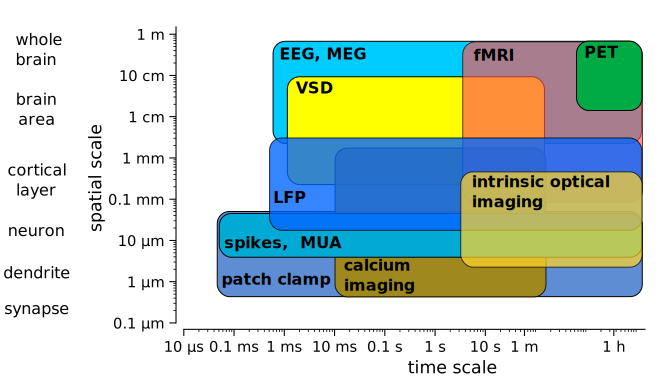
\includegraphics[width=1.0\textwidth]{Figures/Intro/measurement_scales_in_neuroscience.pdf}
\end{center}
\caption[]{\textbf{Overview of measurements of neural activity}}
\label{Intro:fig:Measurements}
\end{figure}
%%%

%%%
\begin{figure}[!ht]
\begin{center}
\includegraphics[width=1.0\textwidth]{Figures/Intro/ecs_nano_2.png}
\end{center}
\caption[]{\textbf{ECS}}
\label{Intro:fig:ECS-sketch}
\end{figure}
%%%

\section{\red{GH: The brain is electric}}
The main functional unit in the brain is the neuron. There are many different kinds of neurons. Some tend to increase the activity of other neurons, and these are called excitatory neurons, while others tend to decrease the activity of other neurons, and are called inhibitory neurons. Different kinds of neurons also vary in terms of their morphology. So-called pyramidal cells, for example, tend to form long nerve fibre branches (dendrites) in a preferred spatial direction, from the bottom towards the top of laminar parts of the brain, such as cortex and hippocampus. Other neurons, such as spiny stellate cells, have more spherically symmetric morphologies. The different kinds of neurons also vary in terms of their dynamical properties, i.e., in terms of how they respond to particular kinds of inputs.

As indicated in Fig. \ref{Basics:fig:Basics}A, the neural morphology can be divided into three functionally different parts: The \textit{soma}, the \textit{dendrites} and the \textit{axon}. The synapses, through which a neuron receives input from other neurons, are predominantly distributed over its dendrites, which are long and branchy extrusions from the soma. A single neuron may have synaptic connections from thousands of other neurons, and can receive input from several of them at the same time. These inputs are sensed, or "integrated" by the soma, which, depending on the net input, decides whether or not the neuron produces an output signal. The axon is another type of extrusion from the soma, which forms synapses onto the dendrites of other neurons. When the neuron produces an output signal, an electric pulse will travel along the axon and reach the synaptic location, where the (presynaptic) output from one neuron becomes the (postsynaptic) input to another.

When a neuron rests, i.e., when it receives no input from any other neuron, its membrane potential has a negative value. The exact value varies between different neuron species, but a typical value could be $-70$ mV. When it receives inputs from other neurons, the membrane potential is jolted away from the resting potential. If the input is sufficiently strong to drive it above a certain threshold, which is often around $-50$ mV, although also this may vary between different neuron species, a set of intrinsic membrane mechanisms called ion channels will be activated. The are basically pores that open in the membrane, allowing charged particles (ions) to rush into and out from the neuron in a systematic manner to charge up and de-charge the membrane.
The sum of these transmembrane fluxes produce a so-called action potential, a sharp spike in the voltage which peaks at some positive value of for example $+20$ mV. The action potential is the main output signal of a neuron, and the basic signaling unit in the brain.

The dynamics of the membrane potential of a neuron can be recorded experimentally with an electrode inserted into the soma of the neuron (Fig. \ref{Basics:fig:Basics}A). Such recordings will give us good insight into the dynamics of the single neuron from which it is recorded. However, if we are trying to answer some question relevant at a more systemic level, such as "how is the visual cortex processing a particular type of visual inputs?", the doings of a single neuron might not give us too much insight.

As it is experimentally challenging to record intracellularly from more than one, or at least from more than a few, neurons at the same time, many experimental studies are instead based on using extracellular recordings. An electrode is then inserted, for example, into the brain tissue amidst the jungle of neurons that the experimentalist wants to know something about (Fig. \ref{Basics:fig:Basics}B). The signal recorded with an extracellular electrode will reflect the activity of a large number of neurons, and the interpretation of this signal is not as straightforward as the interpretation of an intracellular recording. In order to interpret extracellular recordings we therefore need a theory that relates what a population of neurons is doing to what an electrode placed amidst them, or at some distance away from them, measures. The objective of this book is present such a theory.





\section{\orange{GH: Overview the contents in this book}}
This book is divided into two parts. In Part 1 we introduce the theory for modeling neurons and the extracellular potential that they give rise to, and in Part 2 we apply this theory to extract key insights about how to interpret extracellular potentials in terms of what aspects of neural activity that they reflect.

Throughout most parts of this book, we shall compute extracellular potentials using a two-step procedure:

\begin{itemize}
\item {\bf Step 1:} Compute the electrical activity of the cells believed to contribute to the extracellular potential.
\item {\bf Step 2:} Compute the extracellular potential that arises from a given, underlying cellular activity.
\end{itemize}

Following this two-step procedure, Chapter \ref{sec:Neuron} describes how to model and compute the dynamics of morphologically complex neurons (step 1), and Chapter \ref{sec:VC} describes how to compute the resulting extracellular potential (step 2). The computations in step 2 depend on the extracellular medium, as reflected through its conductivity $\sigma$. Chapter \ref{chap:Sigma} is devoted to present experimental and theoretical estimates of $\sigma$, and to explain how various choices for $\sigma$ can be incorporated into the theory (step 2). Taken together, chapters \ref{sec:Neuron}-\ref{chap:Sigma} contain the theory used for all simulations in the application part (Part 2) of this book, which remains the standard theory used within the field of neuroscience to simulate extracellular potentials.

The standard theory (covered by Chapters \ref{sec:Neuron}-\ref{chap:Sigma}) assumes (1) that ion concentrations in the extracellular (and intracellular) environment do not vary with time. This is thought to be a good approximation during normal cellular activity. However, extracellular ion concentration shifts are a trademark of many pathological conditions such as epilepsy, stroke or spreading depression \cite**{Somjen2001,Frohlich2008,Zandt2015,Ayata2015}. In Chapter \ref{sec:Eldiff} we expand step 2 by outlining a theory for modeling extracellular ion concentration dynamics surrounding active neurons, and the effects that this will have on the extracellular potential. 

The standard theory also assumes (2) that the extracellular potential (computed in step 2) does not have any feedback effect on the neurodynamics (computed in step 1). The justification making such an assumption is that $\phi$ is usually so much smaller than the membrane potential such, so-called ephaptic effects can be neglected without any severe loss in accuracy. Also, assuming this, simplifies the mathematical framework, and speeds up computations substantially.

In reality, both in the the extracellular potential and in the extracellular ion concentrations will in principle affect the neurodynamics. Although these effects may be small for most scenarios, there are also scenarios where the assumptions (1)-(2) do not hold, so that the standard two-step procedure can not be applied. We therefore end the theory part (Part 1) of this book by giving a summary of alternative available frameworks for computing extracellular potentials and ion concentrations (Chapter \ref{sec:Schemes}).

In the application part (Part 2) of this book, we use the theory from Part 1 to simulate extracellular potentials at different levels through forward modeling. By \textit{forward modeling} we here mean that start off with a system of neurons that is supposed to mimic a physiologically realistic scenario, and then use this predict the resulting extracellular potential, i.e., a signal that one can measure experimentally. The opposite approach, \textit{inverse modeling}, would be to try to predict the system of neurons or some properties from it from a (measured) extracellular potential. \textit{Inverse modeling} is more problematic than forward modeling, as it has no unique solution, and we will not deal with this in this book.

The motivation behind forward models is multifold. Firstly, if the model system generates an extracellular potential similar to that measured in given experimental condition, it gives validity to the model system. Secondly, by manipulating aspects of the model system, such as neuronal morphology, synapse distributions, neural membrane mechanisms etc., and exploring the effects that this has on the extracellular potential, we may gain knowledge into how various aspects of neuronal dynamics are involved in shaping the extracellular potential. As such, forward modeling gives us insights that can be used to interpret experimentally recorded extracellular potentials.

What the extracellular potential tells us about the underlying neurodynamics depends on where it was recorded, and what aspects of it that we look at, e.g., if we look at the fast variations of it (high-frequency component), or slower variations (low-frequency component). Part 2 is organized so that we first consider the extracellular potential close to its sources, i.e., amidst the forest of neurons, which can be recorded experimentally with sharp electrodes inserted into the brain tissue. By performing a filtering of this signal, we can split it into a high-frequency part and a low-frequency part. In Chapter \ref{chap:Spikes} we examine the high-frequency part, often called the multi-unit-activity (MUA), and show that this mostly reflects the population spiking activity. In In Chapter \ref{sec:LFP} we focus on the low-frequency part, and show that this mostly reflects synaptic input to populations of pyramidal cells.

In the following chapters, we study the extracellular potential at positions further away from their neuronal sources. In Chapter \ref{sec:ECoG}, we the electrocorticogram (ECoG), measured at the surface of the cortex, or the electroencephalogram (EEG) measured at the top of the scalp. We also include a chapter (Chapter \ref{sec:MEG}) on the magnetoencephalogram, which can be modeled on a framework similar to that used for EEG.

The theory for how electrical potential propagate from neural sources to a recording electrode can, of course, also be applied to predict how signals will propagate from artificial sources such as stimulus electrodes. In Chapter \ref{sec:Stim} we briefly present a framework for this, as it will be useful in the context of understanding brain stimulations with e.g., deep electrodes.

Finally, we discuss the state of the art technology for brain recordings, and comment on future outlooks and people like Elon Musk (Chapter \ref{sec:Tech}), before we end  by giving a summary of the main take-home messages from this book (Chapter \ref{sec:Last}).

\section{Basic concepts} 
\label{sec:Basics}
Action potentials and extracellular potentials are electric signals, and to understand them, we need to have some basic knowledge about the physics of electricity. 

The overview given here will ...


\subsection{\orange{GH: The physics}}


\subsubsection{\orange{GH: Electric charge}}
The fundamental quantity for electricity is the charge carried by the protons and electrons that build up the atoms that build up the material world. The proton has a charge $e$, while the electron has a charge $-e$, where $e = 1.602\times10^{-19}$ Coulomb (C) is the unit charge. 

In the brain, the charge carriers are not free electrons (or protons), but ions. Ions are atoms or molecules that have gained or donated one or several electrons, and therefore have become electrically charged. Important charge carriers in the brain are Na$^+$, K$^+$ (with charge $e$), Cl$^-$ (with charge $-e$), and $Ca^{2+}$ (with charge $2e$), which are floating around in the saline solutions that fill both the intracellular and extracellular space.

Starting at a fundamental level, a pair of charges, $q'$ and $q$, will act on each others with a force given by Coulomb's law:

\begin{equation}
F = k_e\frac{q q'}r^2, 
\label{Basics:eq:CoulombF}
\end{equation}
where $k_e = 8.99\times10^9$ N$\cdot$ m$^2\cdot$C$^{-2}$ is Coulomb's constant, and $r$ is the distance between the two charges. The direction of the force is along the line between the two charges, and the force will be repelling if the charges have the same valency (sign) and attractive if they have the opposite valency. 

If there are several point charges present, the contribution from each of them sum up linearly. We can then use Coulomb's law to compute the net force that will act on one charge $q$ in a position ${\bf r}$, by summing the contributions from all other charges $q_1, q_2, q_3 ... q_N$ in positions ${\bf r_1}, {\bf r_2}, {\bf r_3} ... {\bf r_N}$: 
\begin{equation}
{\bf F}({\bf r}) = \sum_{n=1}^N k_e q q_n \frac{{\bf r}-{\bf r_n}{|{\bf r}-{\bf r_n}|^3}.
\label{Basics:eq:CoulombFN}
\end{equation}
We have here used a boldface notation to indicate that the force and positions are vectors, entities that have both a magnitude and spatial direction. The position vector ${\bf r}$ can be visualized as an arrow from a reference point $r=0$ to the position of the charge $q$. Likewise, the vector ${\bf r}-{\bf r_n}$ as an arrow between the positions of the charge pair $q$ and $q_n$, defining both the distance and direction of the (imagined) line connecting them.

If our system of study consisted of a small number $N_{small}$ of charges, we could use $N_{small}$ instances of eq. \ref{Basics:eq:CoulombFN} to compute the force acting on each individual charge. Together with Newton's law ${\bf F} = m {\bf a}$, which tells us how the charges will be accelerated in the force direction, eq.\ref{Basics:eq:CoulombFN} would then allow us to compute the movements of all our charges over time. However, when trying to understand what is going on in the brain, we are usually not interested such microscopic interactions between a small number of charges, but rather the joint interactions of a very, very large number of particles. It is then not feasible to keep track of the motion of each individual charge. 

At the larger scale, it is therefore more useful to work with electric fields, which we will define below. It is still nice to have taken a look at  Eq. \ref{Basics:eq:CoulombFN}, since it establishes the fundamental origin of electrical forces and fields. 


\subsubsection{\orange{GH: Electric fields}}
The electric field can be defined as the force that will act on a reference charge $q$, i.e., 
\begin{equation}
{\bf E}({\bf r}) = {\bf F}({\bf r})/q.
\label{Basics:eq:E}
\end{equation}

In general, an electric field can originate either from electric charges, or from time-varying magnetic fields. However, we shall assume that the problems that we deal with in this book are \textit{quasi-electrostatic}, which means that the latter contribution can be neglected. Electric fields are then exclusively due to the forces given by eq. \ref{Basics:eq:CoulombFN}, and by inserting eq. \ref{Basics:eq:CoulombFN} into eq. \ref{Basics:eq:E}, we get:
\begin{equation}
{\bf E}({\bf r}) = \sum_{n=1}^N k_e q_n \frac{{\bf r}-{\bf r_n}{|{\bf r}-{\bf r_n}|^3}.
\label{Basics:eq:CoulombEN}
\end{equation}

Eq. \ref{Basics:eq:CoulombEN} is valid down to a microscopic level, and the field predicted by it will fluctuate vividly on a very fine spatial scale. It will be big at all locations that are close to a charge (i.e., where ${|{\bf r}-{\bf r_n}|$ for some $n$ is small), and smaller at points where the distance to the nearest charge is longer. As we argued in the previous subsection, it is not a feasible to keep track of each individual charge in a macroscopic system. Apart from revealing the origin of the electrical field, eq. \ref{Basics:eq:CoulombEN} is therefore not very useful for us. 

Fortunately, these microscopic field fluctuations are not of too much interest for us when trying to understand the brain. The electrodes that we use when recording brain signals have a spatial extension, and their tip diameter are typically on the order of a micrometer or so. Hence, when we record some signal in the brain, we practically record the average signal over an electrode surface of, say, a square micrometer. 


Experimentally, when we insert an electrode into the brain, the electrode has some spatial extension. 

The diameter of a typical electrode may be in the order of some micrometers, which 





The field given by 

{\bf r}-{\bf r_n}







\subsubsection{\orange{GH: Electric potentials}}
An often more practically useful concept that the electrical field, is the electrical potential $\phi$ (with units Volt (V)), which is what we normally measure experimentally when we stick an electrode into the brain. In the quasi-static regime, the electric field can be expressed as the spatial derivative of the potential:
\begin{equation}
{\bf E}(x,y,z) = - \nabla \phi(x,y,z) = - \left(\frac{d\phi}{dx} {\bf i}  + \frac{d\phi}{dy} {\bf j} + \frac{d\phi}{dz} {\bf k} \right)
\phi 
\label{Basics:eq:EV}
\end{equation}
The spatial derivative $\nabla$ computes how much a property changes in the various spatial directions, and ${\bf i}$, ${\bf j}$ and  ${\bf k}$ are the unit vectors in the three spatial directions $x$, $y$ and $z$, respectively. 

To get an intuitive understanding of the electric potential, it helps to consider an idealized one-dimensional scenario with a constant field in the $x$-direction. Then, eq. \ref{Basics:eq:EV} simplifies to,
\begin{equation}
E(x) = -\frac{d\phi(x)}{dx} = -\frac{\Delta \phi}{\Delta x} = -\frac{\phi(x_b)-\phi(x_a)}{x_b-x_a},
\label{Basics:eq:EV1D}
\end{equation}
where the first equality follows from the 1D-assumption, the second from the assumption that $E$ is constant, and the third is simply a definition of the second, where $x_b$ and $x_a$ may represent any two arbitrary points in space. For example, if $E = 1$ V/m, and if the distance between our points $x_b-x_a$ is 1m, Eq. \ref{Basics:eq:EV1D} tells us that $\phi$ will be 1 V  lower in $x_b$ compared to $x_a$.

The motivation for introducing the last example, was that we wanted use it to make a comment on \textit{grounding}. In the example, the same field $E$ can be obtained with any pair of potentials $\phi_a$ and $\phi_b$ as long as the difference between them is 1 V. We can therefore not speak of the potential as an absolute quantity, only of the potential \textit{difference} between two points. When we record potential in a given location, we therefore always record it relative to some an arbitrary reference point, which we normally call \textit{ground}, and where we define $\phi = 0$. When recording extracellular potential, the reference electrode can be placed either outside or inside brain tissue \cite{Sharott2015}, but typically sufficiently far away that one can assume that the potential at the reference electrode is not affected by the processes that one wishes to investigate with the measuring electrode. 


\subsubsection{\orange{GH: Electric current}}

Eq. \ref{Basics:eq:CoulombE}

\ref{Basics:eq:CoulombE2}

A test charge $q$ in a medium will of course be exposed to the fields from a large number of other charges. 





The force that a charge excerts on other charges can be expressed as an electric field.

A charge is surrounded by 

Fundamentally, the electric field can be defined as the force that will act on a reference charge $q$, i.e., ${\bf E} = {\bf F}/q$. Now, if we existed in a vacuum where $q$ was the only charge present, this relation implies that a constant field ${\bf E}$ would give a constant acceleration of $q$ (since ${\bf F} = m{\bf a}$) in the field-direction. 

In a macroscopic system, however, the constant acceleration will only go on for a very tiny time period (called the charge relaxation-time) before our protagonist charge $q$ will bump into some other particle and be scattered out in some random direction. After the scattering event, the acceleration will start "from scratch" again, and go on until the next collision takes place, and so on. Whereas the scattering events will make the motion of $q$ random, the small periods of acceleration between them will at average give $q$ a net drift velocity in the field direction. As the same will happen for all other charges that are present, this gives rise to a drift of charge in field direction. This (average) drift will not be in constant acceleration, but rather at constant velocity, and is what constitutes the current density given by Eq. \ref{Basics:eq:i}, which is often referred to as the drift current density. 


In addition to originating from 




\subsubsection{\orange{GH: Currents}}

What we deal with at a more macroscopic level is therefore usually the "average" movement of the charges, i.e., the electrical current ${\bf I}$, which has the SI unit Ampere (A = C/s). It is often more convenient to express currents as current densities, ${\bf i}$ (A/(m$^2$)), which is simply the current per unit cross section area. 

Throughout most of this book, we shall assume that current densities are given by the formula:
\begin{equation}
{\bf i} = \sigma {\bf E}
\label{Basics:eq:i}
\end{equation}
which is a version of Ohms law that, apart from the current density, contains two fundamental quantities that we need to establish an understanding of. The conductivity $\sigma$ (with units Siemens per square meters (S/m$^2$)) expresses how well the medium conducts a current. This is a material property, and in brain tissue, it is often assumed to be a constant, at least within a given brain region. The electric field {\bf E} (with units Newton per Coulomb (N/C) or Volt per meter (V/m)) is the driving force for the current.


\subsubsection{\orange{GH: From neurodynamics to electric fields}}
The link between neural activity and the extracellular fields, come from the fact that currents generally move in loops. 





\subsection{\orange{GH: The physics}}
The basic unit for the physics of electricity is the unit charge. 


\subsection{\orange{GH: The mathematics}}
The basic unit for mathematics is the number 1.




This book is divided into two parts. In Part 1 we introduce the theory for modeling neurons and the extracellular potential that they give rise to, and in Part 2 we apply this theory to extract key insights about how to interpret extracellular potentials in terms of what aspects of neural activity that they reflect.

Throughout most parts of this book, we shall compute extracellular potentials using a two-step procedure:  

\begin{itemize}
\item {\bf Step 1:} Compute the electrical activity of the cells believed to contribute to the extracellular potential. 
\item {\bf Step 2:} Compute the extracellular potential that arises from a given, underlying cellular activity.
\end{itemize}

Following this two-step procedure, Chapter \ref{sec:Neuron} describes how to model and compute the dynamics of morphologically complex neurons (step 1), and Chapter \ref{sec:VC} describes how to compute the resulting extracellular potential (step 2). The computations in step 2 depend on the extracellular medium, as reflected through its conductivity $\sigma$. Chapter \ref{sec:Sigma} is devoted to present experimental and theoretical estimates of $\sigma$, and to explain how various choices for $\sigma$ can be incorporated into the theory (step 2). Taken together, chapters \ref{sec:Neuron}-\ref{sec:Sigma} contain the theory used for all simulations in the application part (Part 2) of this book, which remains the standard theory used within the field of neuroscience to simulate extracellular potentials. 

The standard theory (covered by Chapters \ref{sec:Neuron}-\ref{sec:Sigma}) assumes (1) that ion concentrations in the extracellular (and intracellular) environment do not vary with time. This is thought to be a good approximation during normal cellular activity. However, extracellular ion concentration shifts are a trademark of many pathological conditions such as epilepsy, stroke or spreading depression \citep{Somjen2001, Frohlich2008, Zandt2015review, Ayata2015}. In Chapter \ref{sec:Eldiff} we expand step 2 by outlining a theory for modeling extracellular ion concentration dynamics surrounding active neurons, and the effects that this will have on the extracellular potential. 

The standard theory also assumes (2) that the extracellular potential (computed in step 2) does not have any feedback effect on the neurodynamics (computed in step 1). The justification making such an assumption is that $\phi$ is usually so much smaller than the membrane potential such, so-called ephaptic effects can be neglected without any severe loss in accuracy. Also, assuming this, simplifies the mathematical framework, and speeds up computations substantially. 

In reality, both in the the extracellular potential and in the extracellular ion concentrations will in principle affect the neurodynamics. Although these effects may be small for most scenarios, there are also scenarios where the assumptions (1)-(2) do not hold, so that the standard two-step procedure can not be applied. We therefore end the theory part (Part 1) of this book by giving a summary of alternative available frameworks for computing extracellular potentials and ion concentrations (Chapter \ref{sec:Schemes}).

In the application part (Part 2) of this book, we use the theory from Part 1 to simulate extracellular potentials at different levels through forward modeling. By \textit{forward modeling} we here mean that start off with a system of neurons that is supposed to mimic a physiologically realistic scenario, and then use this predict the resulting extracellular potential, i.e., a signal that one can measure experimentally. The opposite approach, \textit{inverse modeling}, would be to try to predict the system of neurons or some properties from it from a (measured) extracellular potential. \textit{Inverse modeling} is more problematic than forward modeling, as it has no unique solution, and we will not deal with this in this book.

The motivation behind forward models is multifold. Firstly, if the model system generates an extracellular potential similar to that measured in given experimental condition, it gives validity to the model system. Secondly, by manipulating aspects of the model system, such as neuronal morphology, synapse distributions, neural membrane mechanisms etc., and exploring the effects that this has on the extracellular potential, we may gain knowledge into how various aspects of neuronal dynamics are involved in shaping the extracellular potential. As such, forward modeling gives us insights that can be used to interpret experimentally recorded extracellular potentials. 

What the extracellular potential tells us about the underlying neurodynamics depends on where it was recorded, and what aspects of it that we look at, e.g., if we look at the fast variations of it (high-frequency component), or slower variations (low-frequency component). Part 2 is organized so that we first consider the extracellular potential close to its sources, i.e., amidst the forest of neurons, which can be recorded experimentally with sharp electrodes inserted into the brain tissue. By performing a filtering of this signal, we can split it into a high-frequency part and a low-frequency part. In Chapter \ref{sec:Spikes} we examine the high-frequency part, often called the multi-unit-activity (MUA), and show that this mostly reflects the population spiking activity. In In Chapter \ref{sec:LFP} we focus on the low-frequency part, and show that this mostly reflects synaptic input to populations of pyramidal cells.

In the following chapters, we study the extracellular potential at positions further away from their neuronal sources. In Chapter \ref{sec:ECoG}, we the electrocorticogram (ECoG), measured at the surface of the cortex, or the electroencephalogram (EEG) measured at the top of the scalp. We also include a chapter (Chapter \ref{sec:MEG}) on the magnetoencephalogram, which can be modeled on a framework similar to that used for EEG. 

The theory for how electrical potential propagate from neural sources to a recording electrode can, of course, also be applied to predict how signals will propagate from artificial sources such as stimulus electrodes. In Chapter \ref{sec:Stim} we briefly present a framework for this, as it will be useful in the context of understanding brain stimulations with e.g., deep electrodes. 

Finally, we discuss the state of the art technology for brain recordings, and comment on future outlooks and people like Elon Musk (Chapter \ref{sec:Tech}), before we end  by giving a summary of the main take-home messages from this book (Chapter \ref{sec:Last}).


\part{Theory}
\chapter{Theory: Neural dynamics}
\label{sec:Neuron}
\label{chap:Neuron}
\index{Multicompartmental neuron model}
The main contribution to extracellular potentials comes from the electrical activity of neurons. To model extracellular potentials, we therefore first need a model of the neurons generating them. Moreover, a neuron's contribution to the extracellular potential depends strongly on its morphology, 
meaning that we will need multicompar\ehtxt{t}mental 
neuron models \index{Multicompartment model} that account for the neuron's spatial extension.

Modeling of neurons is at the core of computational neuroscience. There exist many types of frameworks for constructing neuronal models at various levels of detail and abstraction, and the topic has been treated in detail in several text books (see e.g.,\cite**{johnston1994foundations,KockSegev1998,Koch1999,DeSchutter2000,Hille2001,Dayan2005,Izhikevich2007,Sterratt2011,Miller2018}). We shall here give only a rather brief introduction to the topic, and we shall limit ourselves to present the most standard kind multicompartmental neuron model, based on a framework which combines a so-called Hodgkin-Huxley type description of the neural membrane mechanisms (see e.g., \cite**{Hodgkin1952,KockSegev1998,Pospischil2008}) with cable theory to predict how signals propagate spatially in dendrites and axons (see, e.g., \cite**{Koch1999,rall2011}). We shall refer to this framework simply as the multicompartment (MC) framework. The MC framework has become the gold standard for biophysically detailed neuronal simulations on the cellular and network level, and has been used for simulating the dynamics of large neuronal networks (see e.g., \cite**{traub2005,markram2015,arkhipov2018}).

A MC model is characterized by (i) its morphology, and (ii) its membrane mechanisms, and the key dynamical variable is the membrane potential (V). The morphology (i) of the real neuron (Fig. \ref{Neuron:fig:multicomp}A) is represented as a discretized set of compartments connected by resistors (Fig. \ref{Neuron:fig:multicomp}B), and there are two categories of currents which together determine the membrane potential dynamics in the compartments (Fig. \ref{Neuron:fig:multicomp}C). These are the currents that run intracellularly between compartments (yellow arrows), and the transmembrane currents at each compartment (green arrows), which are determined by a set of (ii) neuron specific membrane mechanisms. Once all the currents are characterized, the dynamics of the membrane potential can be computed by Kirchhoff's current law, which demands that the sum of currents into a given compartment is zero.

\begin{figure}[!ht]
\begin{center}
\includegraphics[width=0.6\textwidth]{Figures/Neuron/multicompartment.png}
\end{center}
\caption{\textbf{Multicompartmental modelling.}  (A) The neural morphology is (B) represented by a multicompartmental model, where the compartments are treated as cylinders connected by resistors. The example shows a crudely simplified model containing only five compartments, but detailed multicompartment models may include several hundreds of compartments, and can represent t he morphology in great detail. (C) Electric currents in the model can be separated into two groups: (i) transmembrane current in a compartment (green arrows), and (ii) intracellular currents between compartments (yellow arrows). 
}
\label{Neuron:fig:multicomp}
\end{figure}

To present the MC framework, we will start by presenting a framework for modeling the transmembrane currents in a single compartment (Section \ref{sec:Neuron:membranecurrents}), and next show how a number of such compartments can be connected together to a MC model (Section \ref{sec:Neuron:morphology}). Together, those two sections provide a theoretical framework for modeling neurons that should be sufficient for most practical applications. Readers that crave further biophysical insight into the ionic movements that actually give rise to the transmembrane neural currents can get a brief introduction to this in Section\ref{sec:Neuron:Ions_and_reversals}. Finally, we end the chapter about neuronal modeling by briefly summarizing the main assumptions underlying the HHC (Section \ref{sec:Neuron:HHCassumptions}).


\section{\blue{Membrane currents}}
\label{sec:Neuron:membranecurrents}
\index{Hodgkin-Huxley type model}
Hodgkin-Huxley (HH) type models are called so because they describe the membrane mechanisms with a mathematical formalism similar to that used in celebrated model by \citeasnoun**{Hodgkin1952}. In HH-type models, the membrane typically includes three autonomous classes of transmembrane currents, normally represented as current densities (unit mA/cm$^2$). These are (i) a capacitive current density ($i_c$), (ii) a the leakage current density ($i_L$), and (iii) a the current density through active ion channels ($i_x$), of which there may be several different kinds ($x$ is an index). 
\ehnote{Notasjon boer ryddes opp i. Kursiv subfix boer representere index, mens subfix som er en forkortelse (c-capacitance, m-membrane etc.) skal ikke vaere kursiv men normal font: $i_\mathrm{m}$.}
In addition, a neuron may receive  (iv) external stimuli ($i_{stim}$) either through synaptic currents or experimental current injections. In the case where the neuron is modeled as a single compartment, the net transmembrane current must be zero, so that:

\begin{equation}
i_c + i_L + \sum_x{i_x} +  i_{stim} = 0.
\label{Neuron:eq:singlecomp_zerosum}
\end{equation}
Below, we define the various currents that go into this equation.


\subsection{\blue{Capacitive current}}
\label{sec:Neuron:Cap}
\index{Capacitive current}

The capacitive current density,
\begin{equation}
i_c = c_m \frac{dV}{dt},
\label{Neuron:eq:HHcap}
\end{equation}
represents the charging up of the membrane potential $V$ due to a charge density accumulating on the outside of inside of the capacitive membrane. Here, $c_m$ is the specific membrane capacitance. In the original HH-model, $c_m$ had the value
1 $\mu$F/cm$^2$, and this value seems to be representative for most neurons.  An illustration of how to interpret the capacitive current is given in Fig. \ref{Neuron:fig:capacitive_currents}. 

\begin{figure}[!ht]
\begin{center}
\includegraphics[width=0.8\textwidth]{Figures/Neuron/capacitive_currents.pdf}
\end{center}
\caption{\textbf{Capacitive currents are important for current conservation.}  (\textbf{(A)}) The extracellular and intracellular bulk solutions are essentially electroneutral, and the only region where there is a nonzero charge density is in thin Debye layers around the capacitive membrane. Unlike the other currents involved, the capacitive current is not due to ions crossing the membrane, but due to ions piling up on either side of it, separating a membrane charge density $\eta$ and a charge membrane charge density $-\eta$, giving rise to a membrane potential of $V = \eta/c_m$. An outward capacitive current could correspond to an anion leaving the membrane on the inside (\textbf{(B)}), which will coincide with a cation leaving the membrane on the outside (\textbf{(C)}). Thus, capacitive membrane currents do give rise to electrical ionic volume currents both in the intra- and extracellular space.
}
\label{Neuron:fig:capacitive_currents}
\end{figure}

If we insert eq. \ref{Neuron:eq:HHcap} into eq. \ref{Neuron:eq:singlecomp_zerosum}, we get:
\begin{equation}
c_m \frac{dV}{dt} = - (i_L + \sum_x{i_x} +  i_{stim}),
\label{Neuron:eq:singlecomp_capinserted}
\end{equation}
which may give us an intuitive understanding of neurodynamics: If the sum of ionic currents over the membrane (right hand side) is nonzero, it will lead to a charging up (left hand side) of the membrane. 


\subsection{\blue{Leakage current}}
\label{sec:Neuron:leak}
\index{Leakage current}

The leakage current density is given by
\begin{equation}
i_L = \bar{g}_L (V - E_L),
\label{Neuron:eq:HHleak}
\end{equation}
where $\bar{g}_L$ (mS/cm$^2$) is the leak conductance (the bar indicates that it's a constant). The factor $(V - E_L)$ (mV) is often called the driving force, and $E_L$ the leak reversal potential. The biophysical origin of the reversal potential is explained later (see Section \ref{sec:Neuron:Ions_and_reversals}). For now, we may simply think of $E_L$ as the "target potential" that the leakage current will strive to drive the membrane potential towards. In reality, the leakage current is not a single current, but represents an orchestra of physiological processes that together will drive the membrane potential towards the value $E_L$. 

Together, the capacitive current and the leakage current determine the passive properties of the membrane. If the neuron were to include only these two currents, it could be well modeled as an RC-circuit, and RC-neuron models are often used to simulate the subthreshold dynamics of neurons (Fig. \ref{Neuron:fig:RC}). 

\begin{figure}[!ht]
\begin{center}
\includegraphics[width=0.8\textwidth]{Figures/Neuron/RCneuron.png}
\end{center}
\caption{\textbf{RC-neuron.}  A neuron model containing only a capacitive and a leakage current can be represented as an RC-circuit. To use standard MC modeling convention, we we have expressed the various variables and parameters in units per membrane area: With a total membrane resistance $R = 1/(g_L A)$, and capacitance $C = c_mA$, we get that $RC = c_m/g_L$. In the illustration, the neuron is given a current injection $i_e$ (A/cm$^2$) and responds by charging up the membrane. When the input is terminated, the membrane potential will return to the value $E_L$. In the RC-model, $E_L$ will be identical to the resting potential of the neuron, i.e., the potential that the membrane will settle on in the case where it does not receive any input. In models which include additional, active ion channels, these can in principle affect the resting potential, so that it may generally differ from $E_L$.
}
\label{Neuron:fig:RC}
\end{figure}


\subsection{\blue{Active ion channels}}
\label{sec:Neuron:active}
\index{Active ion channels}
In addition to $i_c$ and $i_L$, biophysical neuronal models typically include a number of active ion channels. These account for the "fancy" aspect of neurodynamics, and the main legacy of Hodgkin and Huxley was that they derived a mathematical model for describing the kinetics of these \cite**{Hodgkin1952}.

In the HH-type formalism, the current through an active ion channel type $x$ is modeled as:
\begin{equation}
i_x = \bar{g}_x m_x^{\alpha} h_x^{\beta}(V-E_x).
\label{Neuron:eq:HHform}
\end{equation}
We note that the current density $i_x$ does not represent the current through a single ion channel, but a large number of channels of the same type $x$. Thus, $\bar{g}_x$ (mS/cm$^2$) denotes the conductance when all channels of type $x$ are fully open (the bar indicates that it's a constant), while $E_x$ (mV) is the reversal potential for the ion species that travels through the channel type. In analogy with the leak reversal potential, we may think of $E_x$ as the target potential that the current through ion channel $x$ will strive to drive the membrane potential towards. The intrinsic membrane potential dynamics is thus due to the competition between various currents that try to drive it towards their respective reversal potentials. 

If one prefers to think of neurons in terms of circuit diagrams, the active ion channels are simply added in parallel to the passive $i_c$ and $i_L$ currents. As an example, the electric circuit representation of the HH model is depicted in Fig. \ref{Neuron:fig:HH}.

\begin{figure}[!ht]
\begin{center}
\includegraphics[width=0.8\textwidth]{Figures/Neuron/HHmodel.png}
\end{center}
\caption[]{\textbf{Active, single compartment neuron model.}  In addition to a capacitive and a leakage current, active neuron models contain a number of active ion channels. The example diagram shows the original Hodgkin-Huxley model, with an active Na$^+$ and an active K$^+$ channel. The arrows slicing the diagram conductances indicate that they are variables.}
\label{Neuron:fig:HH}
\end{figure}

Active ion channels differ from the passive leakage channel in that their total conductance, $\bar{g}_{x} m^{\alpha} h^{\beta}$, vary with time due to the so-called gating variables, in eq. \ref{Neuron:eq:HHform} denoted $m$ and $h$. These determine the dynamics of how the ion channels activate or deactivate (open or close), and $m$ and $h$ represent two different types of gates differing in terms of their opening/closing dynamics. The exponents $\alpha$ and $\beta$ represent the number of copies that a channel $x$ has of each type of gate. At the level of a single ion channel the values of $m$ and $h$ would interpret as the \textit{probability} that a given gate is in the open state. However, as we here deal with summed currents through a large number of ion channels, the values of $m$ and $h$ interpret as the \textit{fraction} of the gates of the various types that are open. The values are thus numbers between 0 (all gates in the closed state) and 1 (all gates in the open state). The product $m^{\alpha} h^{\beta}$ thus interprets as the fractions of ion channels in which all gates are open so that currents can pass through. The ion channel conductance is thus given by the product $\bar{g}_x m_x^{\alpha} h_x^{\beta}$.

For voltage-gated ion channels, the the dynamics of the gating variables can be described by kinetics equations on the form:
\begin{equation}
\frac{dx(V,t)}{dt} = \frac{x_{\infty}(V) - x}{\tau_x(V)},  \, \text{for } x = \{m,h\}.
\label{Neuron:eq:HHgate}
\end{equation}
Here, the steady state activation $x_{\infty}(V)$, represents the fraction of gates that will end up in the open state if the cell is clamped at a given potential $V$ for sufficiently long time. However, the process of opening the gates takes some time, as accounted for by the activation time constant $\tau_x(V)$ (ms). Both $x_{\infty}(V)$ and $\tau_x(V)$ are functions of the membrane potential, and these must be determined experimentally for each individual ion channel type. We do not go into the experimental challenges here, but will think of them as known functions. 

There are also many ion channels whose activation or inactivation do not depend on $V$, but on some other variable, such as the concentration of some ion species or ligand \cite**{Hille2001,Sterratt2011}. A common example are Ca$^{2+}$ gated ion channels, i.e., channels with gate opening controlled by the intracellular Ca$^{2+}$ concentration ($[Ca^{2+}]_i$). There are also ion channels whose activation depend on more than one variable, such as e.g., ion channels whose activation depend on both $V$ and $[Ca^{2+}]_i$. Fortunately, a HH type formalism can in most cases be applied also to these kind of ion channels, provided that $x_{\infty}(V)$ and $\tau_x(V)$ in eq. \ref{Neuron:eq:HHgate} can be replaced with experimentally determined functions of the relevant variables \cite**{Sterratt2011}. 

To give an example of an active neuron model, the full set of equations for the HH model is summarized in Box \ref{Neuron:box:HH}. Compared to modern biophysically detailed neuron models, the original Hodgkin-Huxley model is relatively simple in that it only contains two (voltage-gated) active ion channels, a Na$^+$ with three activation gates ($m^3$) and one inactivation gate ($h$), as well as a K$^+$ channel with four inactivation gates $n^4$. The two active ion channels are together responsible for action potential generation.  

\begin{floatingbox}[h]
\caption{Hodgkin-Huxley equations}

\begin{eqnarray*}
    c_m \frac{dV}{dt} & =  & -\bar{g}_L(V-E_L) - \bar{g}_{Na} m^3 h (V - E_{Na}) - \bar{g}_{K} n^4 (V - E_{K}) \\
    \frac{dx(V,t)}{dt} & = & \frac{x_{\infty}(V) - x}{\tau_x(V)},  \, \text{for } x = \{m,h,n\} \\ 
    x_{\infty}(V) &= & \frac{\alpha_x(V)}{\alpha_x(V) + \beta_x(V)}, \, \text{for } x = m,n,h \\ %\hline
    \tau_x(V) & = & \frac{1}{\alpha_x(V) + \beta_x(V)}, \, \text{for } x = m,n,h \\ %\hline
    \alpha_n &=& \frac{0.01 \mathrm{ms}^{-1} V+55 \mathrm{mV}}{1-e^{-(V+55 \mathrm{mV})/10 \mathrm{mV}}}  \\ %\hline
     \beta_n &=& 0.125 \mathrm{ms}^-1 e^{-(V+65 \mathrm{mV})/80 \mathrm{mV}}   \\ %\hline
     \alpha_m &=& \frac{0.1 \mathrm{ms}^{-1} V+ 40 \mathrm{mV}} {1-e^{-(V+40 \mathrm{mV})/10 \mathrm{mV}}}  \\   
     \beta_m &=& 4 \mathrm{ms}^{-1} e^{-(V+65  \mathrm{mV})/18 \mathrm{mV}}  \\ %\hline
    \alpha_h &=& 0.07 \mathrm{ms}^{-1} e^{-(V+65 \mathrm{mV})/20 \mathrm{mV}}  \\ %\hline
    \beta_h &=& \frac{1 \mathrm{ms}^{-1}}{1+e^{-(V+35 \mathrm{mV}))/10 \mathrm{mV})}}   \\ %\hline
    c_m &=& 1.0 \mathrm{\mu F/cm^2} \\ %\hline
    \bar{g}{Na} &=& 120 \mathrm{mS/cm^2}\\ %\hline
    \bar{g}_{K} &=& 36 \mathrm{mS/cm^2} \\ %\hline
    \bar{g}_{L} &=& 0.3 \mathrm{mS/cm^2} \\ %\hline
    E_{Na} &=& 50 \mathrm{mV} \\ %\hline
    E_{K} &=& -77  \mathrm{mV} \\ %\hline
    E_{L} &=& -54.4 \mathrm{mV} \\ %\hline
\end{eqnarray*}
\label{Neuron:box:HH}
\end{floatingbox}




\subsection{\blue{Stimulus currents and synapses}}
\label{sec:Neuron:stim}
\index{Stimulus currents}
Finally, the stimulus current in Eq. \ref{Neuron:eq:singlecomp_zerosum}, can represent any external stimulus that a neuron receives. Typically, it is either taken to represent an experimental current injection such as for example a step-current injection:

\begin{equation}
i_\text{inj}(x)= 
\begin{cases}
    constant, & \text{if } t_{start} > t > t_{end} \\
    0,              & \text{otherwise},
\end{cases}
\label{Neuron:eq:injected}
\end{equation}
or a synaptic input. 

The most common synapses are chemical synapses, which are normally modeled more or less like an ion channel:
\begin{equation}
i_\text{syn}(t) = g_\text{syn}(t) \big(V(t)-E_\text{syn} \big), 
\label{Neuron:eq:chemicalsynapse}
\end{equation}
where $E_\text{syn}$ is the reversal potential of the synapse, and $g_\text{syn}(t)$ the conductance. 

The value of $E_\text{syn}$ determines whether a synapse is \textit{excitatory}, which means that it will tend to drive the  membrane potential of neuron toward the threshold for generating action potentials, or \textit{inhibitory}, which means that it will tend to drive the neuron away from the threshold for generating action potentials. Examples of excitatory synapses are AMPA and NMDA synapses, in which $E_\text{syn}$ ($\sim$ 0 - 10 mV) is high above the neuronal resting potential. The most common inhibitory synapse, is the GABA synapse, in which $E_\text{syn}$ ($\sim$ - 70 mV) is close to the resting membrane potential of the neuron.

Unlike for ion channels, which are often voltage or calcium activated, the chemical synapse is activated by neurotransmitters received from a pre-synaptic cell. However, the synaptic response tends to be rather stereotypical, meaning that the post-synaptic response is more or less the same every time the synapse is activated. It is therefore not common to model neurotransmitter activation explicitly. Instead, $g_\text{syn}(t)$ is normally modeled simply as a constant $\bar{g}_\text{syn}$ multiplied with a temporal kernel determining the opening and closing of a synapse set off at an activation time $t_s$. 

Typical choices for $g_\text{syn}(t)$ are \index{Synapse models}: 
\begin{align}
&\text{(i) exponential decay:} \;\; g_\text{syn}(t) = \bar{g}_\text{syn} e^{-(t-t_\text{s})/\tau}\, \Theta(t-t_\text{s}) \\
&\text{(ii) $\alpha$-function:} \;\; g_\text{syn}(t) = \bar{g}_\text{syn} \frac{t-t_\text{s}}{\tau} e^{-(t-t_\text{s})/\tau} \, \Theta(t-t_\text{s}) \\
&\text{(iii) $\beta$-function:} \;\; g_\text{syn}(t) = \bar{g}_\text{syn} \frac{\tau_1 \tau_2}{\tau_1-\tau_2} 
\Big( e^{-(t-t_\text{s})/\tau_1} - e^{-(t-t_\text{s})/\tau_2} \Big) \, \Theta(t-t_\text{s}) \\
& \text{(iv) NMDA-like:} \;\; g_\text{syn}(t) = \bar{g}_\text{syn} \frac{e^{-(t-t_\text{s})/\tau_1} - e^{-(t-t_\text{s})/\tau_2}} {1+\mu [\text{Mg}^{2+}] e^{-\gamma V} } \, \Theta(t-t_\text{s}),
\label{Neuron:eq:synapseforms}
\end{align}
where $\Theta(t)$ is the (Heaviside) unit step function: $\Theta(t \ge 0)=1$,  $\Theta(t< 0)=0$, and where parameters like $\gamma$,  $\tau$, $\tau_1$ and $\tau_2$ must be tuned to experimental data from the particular synapse type that one wants to model. Simple waveform (cf., (i)--(iii) above) typically used for AMPA  and GABA synapses, while the waveform (iv), is mainly relevant for NMDA-synapses, where the conductance is influenced by membrane voltage and concentration of extracellular magnesium. 

\ehnote{Ville lagt til et avsnitt her om stroembaserte synapser her som en forenklet (lineaer) versjon av ovenstaaende som svarer til approksimasjonen} 
$i_\mathrm{syn}(t)=\overline{g}_\mathrm{syn} f(t) (V-E_\mathrm{syn} \overset{(V-E_\mathrm{syn})\approx \mathrm{const.}}{\approx} \overline{i}_\mathrm{syn} f(t)$
\ehnote{da dette vil vaere relevant for hybrid scheme og er ellers en del brukt i punktnettverk.}

In addition to the chemical synapses, some neurons may also be connected directly by electrical synapses called \underline{gap junctions}, where the current from one neural process into the other is simply a function of the voltage difference between them and the conductance: 

\begin{equation}
i_\text{gap}=g_\text{gap} (V_{m2}-V_{m1})
\label{Neuron:eq:gapjunction}
\end{equation}

The strength or efficacy of synaptic transmission may change over time through various processes that are often grouped together under the term "synaptic plasticity". Synaptic plasticity work as a mechanism for learning and memory formation in the brain. It is a much studied topic that has been treated in several text books (see e.g., \citeasnoun**{Joel1993} or \citeasnoun**{Kreutz2012}). We will not go further into this topic here.



%%%%%%%%%%%%%%%%%%%%%%%%%%
\section{\blue{Morphology}}
\label{sec:Neuron:morphology}
\index{Multicompartmental neuron model}
The formalism introduced so far has been for the modeling a neuron as a single compartment. When doing that, one implicitly assumes that the whole neuron is isopotential (same $V$ everywhere). This is generally not true. For example, in neurons with long and branchy dendrites, $V$ in the soma can be completely different from $V$ in the tip of a distal dendrite. To account for the spatial aspect of neuronal signaling, one therefore needs multicompartmental models. The neural morphology is then represented as cylindrical compartments connected with resistors, and $V$ can be computed in each individual compartment (Fig. \ref{Neuron:fig:multikompisen}A). 

\begin{figure}[!ht]
\begin{center}
\includegraphics[width=0.7\textwidth]{Figures/Neuron/multikompis.png}
\end{center}
\caption{\textbf{Multi-compartment model.} {\bf (A)} Representations of a neuronal morphology as a number of interconnected compartments. {\bf (B)} Subset of interconnected compartments. The currents involved in MC modelling include the sum of transmembrane currents ($I^M_n$) in a compartment $n$, and the intracellular currents running between 
compartments, $I_{n-1,n}$ (current from compartment $n-1$ to $n$), and $I_{n,n+1}$ (current from compartment $n$ to $n+1$).}
\label{Neuron:fig:multikompisen}
\end{figure}

As a simple introduction to the formalism used in MC models, let us consider a subset of three connected cylindrical compartments which we number $n-1$, $n$ and $n+1$ (Fig. \ref{Neuron:fig:multikompisen}B). Let us for simplicity assume that the three cylinders have the same length ($L$) and diameter ($d$). The two categories of currents that run in this system are (i) the transmembrane currents that we introduced in the previous subsection, all of which we can group together into a total transmembrane current $I^M_n$, and (ii) the axial currents running between the cylindrical compartments ($I_{n-1,n}$ and $I_{n,n+1}$). The dynamics of this system is computed using Kirchhoff's current law, which demands that the sum of currents into a given compartment ($n$) should be zero:

\begin{equation}
I_{n-1,n} - I_{n,j+1} - I^M_n = 0
\label{Neuron:eq:Kirch}
\end{equation}
We note that we calculate with total currents here (unit A), not current densities, so that $I^M_n$ is the sum of all current densities in the left hand side of eq. \ref{Neuron:eq:singlecomp_zerosum} multiplied with the membrane area of compartment $n$. The axial currents between two compartments are proportional to the voltage difference between the compartments, as determined by Ohms law:
\begin{eqnarray}
I_{n-1,n} = \frac{V_{n-1}-V_n}{4 R_a L/(\pi d^2)}, \nonumber \\ 
I_{n,n+1} = \frac{V_{n}-V_{n+1}}{4 R_a L/(\pi d^2)}.
\label{Neuron:eq:axialcurrents}
\end{eqnarray}
Here, the denominators represent the axial resistance between two compartments, defined in terms of the axial resistivity $R_a$ ($\Omega$ cm), a material property of the cytosol solution, the cross-section area $\pi d^2/4$, and the segment length or travel distance ($L$ (m)). 

The calculations become more complicated when the connected cylinders are of different length and diameter, and especially at branch points. However, the theory for computing the dynamics in branching structures with varying diameters is well established \cite**{Rall1977,Rall1989}, and designated software such as NEURON \cite**{Hines1997,Hines2009} automatizes the compartmentalization for the user once the neural morphology is specified. For the reminder of this chapter, we limit ourselves to consider the simplified, unbranched scenario (Fig. \ref{Neuron:fig:multikompisen}B), as we deem this as sufficient for establishing an understanding of the essentials of morphology modeling. 

We note that in eq. \ref{Neuron:eq:axialcurrents}, $V_n$ is the \emph{intracellular} potential in compartment $n$. However,  we shall in the reminder of this chapter assume that the intracellular potential is identical to the membrane potential in compartment $n$. In practice, that means that we assume that the extracellular space is isopotential and grounded ($V = 0$ there), which may seem like a peculiar assumption to make in a book where the extracellular potential is the main topic. Later, we shall discuss this assumption and its consequences in further detail. For now, we settle with noting that although the extracellular potential in reality is not zero, it is generally so much smaller than the intracellular potential that we can assume that it is zero without going too wrong when computing the neurodynamics. 



%%%%%%%%%%%%
\subsection{\blue{Active multicompartment models}}
\label{sec:Neuron:Active_multicomp}

To specify our MC neuron model further, we write out the total membrane current as:
\begin{equation}
I^M_n = I_n^{cap} + I_n^{ion} + I_n^{stim} = -\pi d L c_m \frac{dV_n}{dt} + \pi d L i_n^{ion} + I_n^{stim}, 
\label{Neuron:eq:Imemb}
\end{equation}
where $I_n^{ion}$ represent the total transmembrane ionic currents through leakage and active ion channels. On the right hand side, we have expressed the capacitive and ionic currents (mA) as current densities (mA/cm$^2$) multiplied with the membrane area ($\pi d L$ (cm$^2$)) represented by the sides of the cylinder, and we have inserted eq. \ref{Neuron:eq:HHcap} for the capacitive current density. If we insert this into Eq. \ref{Neuron:eq:Kirch}, we get:

\begin{equation}
c_m \frac{dV_n}{dt} = i_n^{ion} + \frac{d}{4R_a}\left(\frac{V_{n+1}-V_n}{L^2} - \frac{V_n-V_{n-1}}{L^2} \right) + \frac{I^{stim}}{\pi d L}.
\label{Neuron:eq:multimain}
\end{equation}
For whatever choice of membrane mechanisms that contribute to $i_n^{ion}$, Eq. \ref{Neuron:eq:multimain} can be solved numerically for appropriately chosen boundary conditions. The most common choice for boundary conditions are those of a sealed end ($\frac{\partial V_n}{\partial x} = 0$), or a killed end ($V_n=0$). The NEURON simulator by default uses the sealed-end condition, which means that no axial current leaves at the endpoints of the simulated structure. Eq. \ref{Neuron:eq:multimain} is the fundamental equation for multicompartmental models.



%%%%%%%%%%%%%%%%%
\subsection{\blue{Passive multicompartment models}}
\label{sec:Neuron:Passive_multicomp}
\index{Multicompartmental neuron model}
If the neuron contains no active ion channels, $i_n^{ion} = g_L(V_n - E_L)$ is simply the leakage current density. In purely passive models, the leakage reversal potential is identical to the membrane resting potential, and it is common to denote it by $E_m$. It is then also custom to replace the leak conductance $g_L$ with the membrane resistivity $R_m = 1/g_L$ ($\Omega$ cm$^2$). Eq. \ref{Neuron:eq:multimain} then simplifies to:

\begin{equation}
c_m \frac{dV_n}{dt} = \frac{E_m-V_n}{R_m} + \frac{d}{4R_a}\left(\frac{V_{n+1}-V_n}{L^2} - \frac{V_n-V_{n-1}}{L^2} \right) + \frac{I^{stim}}{\pi d L}
\label{Neuron:eq:multipassive}
\end{equation}

Although all neurons contain some active membrane mechanisms, the passive model (Eq. \ref{Neuron:eq:multipassive}) is still often used as an approximation for signaling in neural dendrites, which tend to have a lower density of active mechanisms compared to the soma and axon. 

An illustration of passive signal propagation shown in Fig. \ref{Neuron:fig:Semiinf}A, which shows the membrane potentials at selected positions along a $1000 \, \mu$m long stick-neuron responding to a stimulus resembling a synaptic input in one end. We see that the peak response comes faster in proximal than in distal locations, and that the peak response decays with distance from the synapse. However, the potential at all points along the cable coincide a few milliseconds after the stimulus was delivered, after which $V$  decays gradually towards the resting potential.

Although the dynamics of course will be system specific, depending on the passive membrane parameters and generally on the presence of active mechanisms, the simulation in Fig. \ref{Neuron:fig:Semiinf}A gives a general, qualitative idea on how signals spread in dendrites. As we shall see below, the passive model is also useful in that it allows us to derive some analytical results for signal propagation in neural branches.

\begin{figure}[!ht]
\begin{center}
\includegraphics[width=0.7\textwidth]{Figures/Neuron/Cablesims.png}
\caption{\textbf{Stick-neuron responding to transient and constant inputs received in one end.} (A) Finite cable of length $L = 1 \, \text{mm}$ simulated numerically as 100 compartments, and stimulated with an alpha-synapse in the first compartment ($0<x<10 \, \mu\text{m}$). Transient responses shown at different distances from the synapse. The peak response decreases with distance from the synapse, and the time to reach the peak increases with distance from the synapse.
(A) Analytical steady-state solution for semi-infinite cable receiving a constant input $I^{stim} = 0.1 \, \text{nA}$ in a sealed end at $x=0$. The membrane potential decays exponentially with distance from the stimulus site.  (A-B) Parameters choices: $c_m=1\,\mu\text{F}/\text{cm}^2$, $d = 1\, \mathrm{\mu}\text{m}$, $R_a=35.4\, \mathrm{\Omega cm}$, $R_m = 10 \, \mathrm{k\Omega cm^2}$, which gives a length constant $\lambda = 840\, \mathrm{\mu m}$. }
\end{center}
\label{Neuron:fig:Semiinf}
\end{figure}


%%%%%%%%%%%%%%%%%%%%
\subsection{\blue{Cable equation}}
\label{sec:Neuron:cableeq}
\index{Cable equation}
If we in Eq. \ref{Neuron:eq:multipassive} let $L \rightarrow \delta x$, and take the limit $\delta x \rightarrow 0$, we obtain the cable equation (see e.g., \cite**{Sterratt2011}): 

\begin{equation}
c_m \frac{\partial V}{\partial t} = \frac{E_m-V}{R_m} +  \frac{d}{4 R_a}  \frac{\partial^2 V}{\partial x^2}  + \frac{\mathcal{I}^{stim}}{\pi d},
\label{Neuron:eq:cable}
\end{equation}
where we have  introduced the stimulus current per unit length, $\mathcal{I}^{stim}(x,t) = I^{stim}(x,t)/\delta x$ (mA/cm). To improve our analytical understanding of dendritic signaling, it is useful to reformulate the cable equation to:
\begin{equation}
\tau_m \frac{\partial V}{\partial t} = E_m-V +   \lambda^2  \frac{\partial^2 V}{\partial x^2}  + \frac{R_m \mathcal{I}^{stim} }{\pi d},
\label{Neuron:eq:cable2}
\end{equation}
where we have multiplied all terms with $R_m$ and introduced the length constant,
\begin{equation}
\lambda = \sqrt{\frac{d R_m}{4 R_a}} \,\; \text{(cm)}, 
\label{Neuron:eq:lengthconst}
\end{equation}
and the time constant, 
\begin{equation}
\tau_m \equiv R_m c_m  \,\; \text{(ms)}.
\label{Neuron:eq:timeconst}
\end{equation}

The cable equation serves as a continuous version of a passive neural branch (with infinitely many infinitely small compartments), where $\tau_m$ is typical time scale (dimensionless time: $t/\tau$), while $\lambda$  is typical length scale  (dimensionless length: $x/\lambda$) for signals in the cable. If a certain point along the cable is perturbed, so that the potential is shifted from rest to a given value $V$, $\tau_m$ will determine how fast the local potential will dissipate back towards rest, while $\lambda$ will tell us how far the local perturbation will spread along the cable. 

Whereas MC models (Eq. \ref{Neuron:eq:multimain} and \ref{Neuron:eq:multipassive}) generally must be solved numerically, the cable equation allows the spatiotemporal evolution of the membrane potential to be solved analytically for some idealized scenarios. Below, we consider a couple of scenarios that will  make the interpretation of $\tau_m$ and $\lambda$ clearer. 


%%%%%%%%%%%%%%%%%%%%
\subsection{\blue{Steady state solution of the cable equation}}
\label{sec:Neuron:cableSS}
Let find the steady state solution for a semi-infinite cable, receiving a constant current injection at the sealed end in $x=0$ (Fig. \ref{Neuron:fig:Semiinf}B). Since only the end-point receives the stimulus, we may attack this problem by solving eq. \ref{Neuron:eq:cable2} for all other points $x>0$, and then introduce the stimulus current as a boundary condition. 

At steady-state, $\partial V/\partial t = 0$, and Eq. \ref{Neuron:eq:cable2} becomes:
\begin{equation}
0 = E_m-V +  \lambda^2 \frac{\partial^2 V}{\partial x^2}, 
\label{Neuron:eq:semiinf}
\end{equation}
at all points along the cable, except $x=0$. If we introduce the new variable $\Delta{V}=V-E_m$, Eq. \ref{Neuron:eq:semiinf} simplifies to:
\begin{equation}
\frac{d^2 \Delta{V}}{d x^2} -  \frac{1}{\lambda^2} \Delta{V}=0, 
\label{Neuron:eq:semiinf2}
\end{equation}
which has the solution:
\begin{align}
\Delta{V}(x) &= \Delta{V}(0) e^{-x/\lambda} \\
V(x) &= E_m + \big( V(0)-E_m \big) e^{-x/\lambda}.
\label{Neuron:eq:semiinf3}
\end{align}
The general-solution to the equation also has a term containing $e^{+x/\lambda}$, but this was excluded on the count of being unphysical, since it diverges when $x \rightarrow \infty$. 

To get the final solution of the problem, we need to specify the boundary value $V(0)$. This will depend on the stimulus current, and since it only exists in a singular point, we go back to expressing in terms of a total current, $I^{stim}$ (and not as a current per unit length $\mathcal{I}^{stim}$). We introduce it through a boundary condition demanding that the injected current (at $x=0$) must be identical to the axial current in the cable at $x=0$:
\begin{equation}
I^{stim} = - \frac{\pi d^2}{4}\frac{1}{R_a} \frac{\partial V}{\partial x}   \Big|_{x=0}.
\end{equation}
The left hand side is the axial cable current as given by Ohm's law. The multiplication with the cable cross section area (first factor on the left) is used to convert a current density to a total current in the cable. If we insert for $\partial V/\partial x$ (calculated from eq. \ref{Neuron:eq:semiinf3}), and insert eq. \ref{Neuron:eq:lengthconst} for $\lambda$, we can derive the following expression for $V(0)$:
\begin{equation}
V(0) = E_m + R_{\infty}I^{stim}, 
\label{Neuron:eq:firstRinf}
\end{equation}
where we have defined:
\begin{equation}
R_{\infty} = \sqrt{\frac{R_m R_a}{\pi^2 d^3}}.
\label{Neuron:eq:Rinf}
\end{equation}
If we insert eq. \ref{Neuron:eq:firstRinf} into eq. \ref{Neuron:eq:semiinf3}, we obtain our final solution:
\begin{equation}
V(x) = E_m +R_{\infty}I^{stim}  e^{-x/\lambda}.
\label{Neuron:eq:semiinf4}
\end{equation}

The steady state solution to the semi-infinite cable (lotted in Fig. \ref{Neuron:fig:Semiinf}B) is useful as it gives us analytical insight into signals spreading in e.g., passive dendrites. Some insights that can be derived from it is:

\begin{itemize}

\item It follows from eq. \ref{Neuron:eq:firstRinf} that $R_{\infty} = (E_m-V(0))/I^{stim}$, and thus interprets as the steady-state input resistance of the semi-infinite cable. Eq. \ref{Neuron:eq:Rinf} thus shows that the input resistance is proportional to $1/d^{3/2}$, i.e., the input resistance is higher the thinner the dendrite. 

\item Eq. \ref{Neuron:eq:semiinf4} shows that in steady-state, the amplitude will decay exponentially from the injection site and outwards, and will be reduced by a factor $1/e$ over the length $\lambda$. If we put in some typical values in eq. \ref{Neuron:eq:lengthconst}, like a dendritic diameter $d=1$~$\mu$m, a membrane resistance of $R_m=10\;\text{k}\Omega\text{cm}^2$, and an axial resistivity $R_a=35.4\;\Omega\text{cm}$, we get a length constant of $\lambda = 840\; \mu$m. Very long dendrites will thus only to a small degree be affected by the membrane potential in the soma.

\item According to eq. \ref{Neuron:eq:lengthconst}, $\lambda \propto \sqrt{d}$, meaning that signals will spread further the thicker the dendrite.

\item According to eq. \ref{Neuron:eq:lengthconst}, $\lambda \propto \sqrt{R_m/R_a}$ meaning that the signal is facilitated by having a large membrane resistance compared to the axial resistance. 

\end{itemize}

\subsection{\blue{Frequency dependence of the cable length constant}}
\label{sec:Neuron:cablefreq}
As we just saw, the length constant $\lambda$ (eq. \ref{Neuron:eq:lengthconst}) is the length over which the potential falls to a fraction $1/e$ of its boundary value when the finite end of a semi-infinite cable is fixed at a constant potential. As this interpretation depends on a constant, direct-current (DC), boundary condition, $\lambda$ is often referred to as the DC length constant. 

It is possible to derive a corresponding length constant for AC input to a semi-infinite cable \cite**{Pettersen2008a}: 
\begin{equation}
\lambda_{AC} = \lambda \sqrt{ \frac{2}{1+\sqrt{(\omega \tau)^2 + 1}} }.
\label{Neuron:eq:AClambda}
\end{equation}
Here $\tau$ still is the membrane time constant (eq. \ref{Neuron:eq:timeconst}), $\lambda$ is still the DC length constant (eq. \ref{Neuron:eq:lengthconst}), and $\omega = 2\pi f$ is the angular frequency of the the boundary potential.

For a constant boundary condition ($I^{stim} = \text{constant}$ in eq. \ref{Neuron:eq:semiinf4}) or, equivalently, $V(0) = \text{constant}$ in eq. \ref{Neuron:eq:semiinf3}), $\omega$ is zero, and we may verify that $\lambda_{AC}$ becomes identical to the DC length constant $\lambda$. For an AC input, we see that $\lambda_{AC}$ decreases with $\omega$, and for high frequencies $\lambda_{AC} \propto (\omega \tau^{-1/2})$. Thus, low frequency input will tend to travel further in dendritic structures, while high frequency input will affect dendritic structures more locally. 

As we shall see later, an important factor determining the size and shape of extracellular potentials is the distance between inward (sinks) and outward (sources) transmembrane currents. This spatial separation is proportional to the neuronal length constant, and from eq. \ref{Neuron:eq:AClambda} we thus know that the source/sink separation will be larger for low frequency components of the neuronal activity.


\subsection{\blue{GH: Temporal solutions of cable equation}}
\label{sec:Neuron:cabletemp}

In Fig. \ref{Neuron:fig:Semiinf}A we simulated numerically the response of a cylindrical neuron to a  synaptic input in one end. It is possible to show analytically that the passive decay of $V$ following the input-induced peaks can be expressed as a sum of exponentials \cite**{rall1969}:
\begin{equation}
V(x,t) = C_0(x) e^{-t/\tau_0} + C_1(x) e^{-t/\tau_1} + C_2(x) e^{-t/\tau_2} + \ldots, 
\label{Neuron:eq:cabletemporal}
\end{equation}
where the coefficients $C_n(x)$ depend on the distance along the cable, while $\tau_0 = \tau_m = R_m c_m$ is the \emph{membrane time constant} (eq. \ref{Neuron:eq:timeconst}), and the other time constants have successively smaller values ($\tau_0 > \tau_1 > \tau_2 > \ldots$). We will not here present these analytical results in any further detail, but note that the final decay phase, i.e., when $V$ at all locations have coincided, takes place at the slower time scale of the membrane time constant, $\tau_m$ which in the simulation in Fig. \ref{Neuron:fig:Semiinf}A  was 10~ms ($R_m=10\,\text{k}\Omega \text{cm}^2$, and $c_m=1\,\mu\text{F}/\text{cm}^2$). 



%%%%%%%%%%


\section{\blue{Ion concentration dynamics and reversal potentials}}
\label{sec:Neuron:Ions_and_reversals}
\index{Ion concentration dynamics}
MC models as defined in Section \ref{sec:Neuron:Active_multicomp} with membrane mechanisms as specified in Section \ref{sec:Neuron:membranecurrents} give a complete and operational framework for modelling the electrical activity of neurons, which works well for most purposes. The reader may chose to skip the remainder of this chapter, which delves more into the biophysical origin of neural activity. 

Up til this point, we have focused on electrical currents in neurons, but talked little of their biophysical origin, i.e., the ions that carry these electrical currents. For example, action potentials are generated by a transmembrane influx of Na\textsuperscript{+}, which charges up (depolarizes) the neuron, followed by an efflux of K\textsuperscript{+}, which decharges (repolarizes) it. These fluxes are primarily driven by diffusion, and thus depend on the intra- and extracellular solutions having different ionic compositions. 

In the neuron models presented in this chapter, it is implicitly assumed that, despite all these various ionic fluxes, the ion concentrations remain constant. This may seem like a peculiar assumption, but it is often quite good. The reason is that the number of ions crossing the membrane during a brief signal such as an action potential only leads to tiny changes in the ion concentrations on either side of the membrane, so that concentrations changes on a short time scale can be neglected. Since neurons possess a team of homeostatic mechanisms that strive to maintain the trans-membrane ion concentration gradients, the assumption of constant ion concentrations also tends to hold on a longer time scale.  The perhaps most important of these mechanisms is the ATPase pump, which uses energy to pump K$^+$ ions into the neuron and Na$^+$ ions out, thus reversing the ionic exchange that occurs during action potential generation. As a result of this pump, the intracellular space tends to remain comparatively rich in K$^+$, while the extracellular space is tends to remain comparatively rich on Na$^+$. Typical values of ion concentrations of the main charge carriers inside and outside neurons are given in Table \ref{Neuron:tab:ion-concentrations}. 

\begin{table}[h]
%\centering
\caption[]{Major charge carrier concentrations inside/outside a typical mammalian neuron. Concentration values were taken from Table 2-1 in \citeasnoun**{Somjenboka} for neurons in the central nervous system (intracellular) and human cerebrospinal fluid (extracellular). Values vary with species and brain regions. Nernst potentials were computed from Eq. \ref{Neuron:eq:revpots} assuming a body temperature of 309.15 K.
}
\label{Neuron:tab:ion-concentrations}
\begin{tabular}{@{}lcccccc@{}}
\hline
					& 	K$^+$	&	Na$^+$	&	Mg$^{2+}$	  &	Cl$^-$	&	Ca$^{2+}$	 	& HCO3$^-$ 	\\ 
\hline
Intracellular (mM)				    & 125		&		10	&		0.5	&	6.6		&  	6$\times$10$^{-5}$	  & 	18 \\
Extracellular (mM)			           & 2.9			&		147	&		0.7	&	119 		&		1	&	23.3	  	\\
Nernst potential (mV)		    &	-100		&	    	+72	&		+4.5	&	-77		&		+129 	& 	-6.9  	\\
\hline
\end{tabular}
\end{table}

In HH-type models, the ensemble of processes that work to maintain baseline conditions are simply assumed to do their job, and not explicitly modeled. Instead, they are grouped together into the \textit{passive} leakage current $I_L$ (eq. \ref{Neuron:eq:HHleak}), which largely determines the cell's resting potential (see see \cite**{offner1991} for a critical study of this approximation). Below, we shall explain how the ionic concentrations are implicitly present in the HH-formalism as they determine the ionic reversal potentials ($E_x$ in eq. \ref{Neuron:eq:HHform}). We shall also comment on the cases where the assumptions of constant ion concentrations are not applicable. 


\subsection{\blue{Ionic reversal potentials}}
\label{sec:Neuron:Erev}
\index{Reversal potential}
Ion channels are pores in the membrane, some of which are selectively permeable only to specific ions. The ion flux through an open ion channel will be mediated by a combination of (i) diffusion and (ii) electric drift. 

For example, when an K$^+$ channel opens, (i) diffusion will strive to drive K$^+$ out from the neuron, since the intracellular space is more K$^+$-rich than the extracellular space, while electric drift will strive to drive K$^+$ into the neuron, since the membrane potential $V$ (defined as intracellular minus the extracellular potential) tends to be negative ($V \sim - 70$  mV during rest). Initially, the diffusive process will dominate, so that the net flux of K$^+$ is outward. This leads to a gradual decrease (hyperpolarization) of the membrane potential,  and a corresponding gradual increase of the drift component. If the K$^+$ channel stays open, the hyperpolarization will go on until the drift component becomes equal in magnitude to the diffusive component, and the net K$^+$ current becomes zero.

The ionic reversal potential is defined as the membrane potential at which the electrical drift current and diffusive current of a given ion species are in an equilibrium, i.e., they are equal in magnitude but oppositely directed. It can be calculated from the Nernst-Planck equation for electrodiffusion \index{Electrodiffusion}. If we approximate the problem as one-dimensional (in the $z$-direction, perpendicular to the membrane), the Nernst-Planck equation for an ion species $k$ is:

%%%%
\begin{equation}
j_k = j_{k,\text{diff}} + j_{k,\text{drift}} 
=  - P_k \Big(\frac{d[k]}{dz} +  \frac{Fz_k}{RT}  [k] \frac{dV}{dz} \Big), 
\label{Neuron:eq:NP1D}
\end{equation}
%%%%
where the first term is Fick's law for the diffusive flux density along the concentration gradient, and the second term is the electrical drift along the voltage gradient. Here, the membrane's permeability ($P_k$) to ion $k$ has taken the role of the diffusion constant ($D_k$) which appears in the more common form of the Nernst-Planck equation. Furthermore, $z_{k}$ is the valency of ion species $k$, $R = 8.314$ J mol$^{-1}$K$^{-1}$ is the gas constant, $F = 96485.3365$ C/mol is Faraday's constant, and $T$ is the absolute temperature (K). The reversal potential (also called the Nernst-potential) is found by solving for when there is no net flux, i.e., when  $j_{k,\text{diff}} = - j_{k,\text{drift}}$:

\begin{equation}
\frac{1}{[k]} \frac{d[k]}{dz} = - \frac{Fz_k}{RT}  \frac{dV}{dz}.
\end{equation}
We may multiply both sides by $dz$ and re-arrange this to get:
\begin{equation}
-dV = \frac{RT}{Fz_k}  \frac{d[k]}{[k]}.
\end{equation}
If we integrate this from the inside to the outside of the membrane, we get:
\begin{align}
-\int_{V_{\text{in}}}^{V_{\text{out}}}  dV &= \frac{RT}{Fz_k}  \int_{[k]_{\text{in}}}^{[k]_{\text{out}}} \frac{d[k]}{[k]} \rightarrow \\
V_{\text{in}}-V_{\text{out}} &= \frac{RT}{Fz_k} ln \frac{[k]_{\text{out}}} {[k]_{\text{in}}} \rightarrow \\
E_k & =  \frac{RT}{Fz_k}  ln \frac{[k]_{\text{out}}} {[k]_{\text{in}}} 
\label{Neuron:eq:revpots}
\end{align}
where the last equality follows from the definition of $E_k$ as the membrane potential $V_{\text{in}}-V_{\text{out}}$ for which the the net flux (in Eq. \ref{Neuron:eq:NP1D}) is zero. Eq. \ref{Neuron:eq:revpots} was used to compute the reversal potentials listed in Table \ref{Neuron:tab:ion-concentrations}. 

As ion concentrations are generally assumed to remain constant in HH-type models, the reversal potentials are also assumed to be constant. As a consequence, one typically do not think that much about ionic concentrations when constructing such models, but simply use values for $E_k$ based or empirical measurements of the potential at which a certain membrane current reverses, i.e., becomes zero.


\subsection{\blue{The Goldman-Hodgkin-Katz equation}}
\label{sec:Neuron:GHK}
\index{Goldman-Hodgkin-Katz equation}
Eq. \ref{Neuron:eq:NP1D} defined the reversal potential for an individual ion species, which is relevant for modeling ion-specific ion channels. To calculate the reversal potential for a non-specific ion channel, we need to express all the individual ion currents separately, and compute the value of $V$ for which they sum to zero. 

If we combine Eq. \ref{Neuron:eq:NP1D} with the assumptions that (i) ions cross the membrane independently, and (ii) that the electrical field within the membrane is constant, we can derive the Goldman-Hodkgkin-Katz (GHK) equation for the membrane currents (see e.g., \cite**{hodgkin1949,johnston1994foundations}):
\begin{equation}
I_\text{k} = P_k z_k F \frac{z_k F V}{R T} \Big( \frac{[k]_\text{in}-[k]_\text{out} e^{-z_k F V/RT}} {1-e^{-z_k F V/RT}} \Big).
\label{Neuron:eq:GHK}
\end{equation}

An example of a non-specific ion channel is the passive leakage current which has a permeability to all ion species simultaneously, so that its reversal potential ($E_L$ in Eq. \ref{Neuron:eq:HHleak}) will depend on all ion concentrations. If we assume that only the three most abundant charge carriers (K$^{+}$, Na$^{+}$ and Cl$^{-}$) contribute, and that they have leak permeabilities $P_K$, $P_{Na}$ and $P_{Cl}$, we can derive from eq. \ref{Neuron:eq:GHK} that they are in equilibrium at the potential:
\begin{equation}
E_L = \frac{R T}{F} 
\ln \frac{P_\text{K} [K]_\text{out}+P_\text{Na} [Na]_\text{out} + P_\text{Cl} [Cl]_\text{in}}
           {P_\text{K} [K]_\text{in}+P_\text{Na} [Na]_\text{in} + P_\text{Cl} [Cl]_\text{out}}.
\label{Neuron:eq:Eleak_GHK}
\end{equation}

Looking at eq. \ref{Neuron:eq:GHK}, we see that the transmembrane currents are nonlinear functions of both the ionic concentrations $[k]$ in the intra and extracellular space, and the membrane potential $V$. In comparison, the transmembrane currents used in the HH-type formalism (eq. \ref{Neuron:eq:HHform}), which are proportional to the driving force $(V-E_k)$, are linearized (sometimes called quasi-Ohmic) versions of the Goldman-Hodkgkin-Katz equation. The HH-form (eq. \ref{Neuron:eq:HHform}) is generally deemed as sufficient for modeling most ion channels, because it gives good predictions of the membrane currents. Ion concentrations and ionic reversal potentials are then assumed to be constant.


\subsection{\blue{Intracellular Calcium dynamics}}
\label{sec:Neuron:Calcium}
\index{Calcium dynamics}
While most ion concentrations are assumed to be constant in HH-based models, it is common to make an exception for Ca$^{2+}$. The main reason for this is that the intracellular Ca$^{2+}$ concentration ($\mathrm{[Ca]_i}$) is very low compared to that of the other ion species (Table \ref{Neuron:tab:ion-concentrations}). Unlike for the other ion species,  $\mathrm{[Ca]_i}$, can therefore change quite dramatically on a short time scale, e.g., during the opening of Ca$^{2+}$ channel. 

The motivations for modeling $\mathrm{[Ca]_i}$ are several. Firstly, to accurately model currents through Ca$^{2+}$ channels, the concentration dependent GHK formalism (eq. \ref{Neuron:eq:GHK}) is often used (see e.g., \cite**{Destexhe1994,Zhu1999,Halnes2011}), and one then needs an expression for $\mathrm{[Ca]_i}$. Secondly, modeling $\mathrm{[Ca]_i}$ could be motivated by the aim to reproduce data from Ca$^{2+}$ imaging experiments. Thirdly, Ca$^{2+}$ does not only act as a charge carrier in neurons, but is also a second messenger, which means that it can trigger a number of intracellular chemical processes, including the gating of Ca$^{2+}$ activated ion channels. 

When Ca$^{2+}$ dynamics is included in HH-based models, it is usually to account for the activation of ion channels that instead of being voltage gated, open or close as a function of $\mathrm{[Ca]_i}$. The kinetics scheme for voltage gated ion channels (\ref{Neuron:eq:HHgate}) \index{Calcium gated ion channels} is then replaced with one dependent on $\mathrm{[Ca]_i}$:

\begin{equation}
\frac{dx(V,t)}{dt} = \frac{x_{\infty}(\mathrm{[Ca]_i}) - x}{\tau_x(\mathrm{[Ca]_i}},  \, \text{for } x = \{m,h\},
\label{Neuron:eq:Cagate}
\end{equation}
and the $\mathrm{[Ca]_i}$ in a neuronal compartment is typically modeled using a simplified framework on the form:
\begin{equation}
\frac{d\mathrm{[Ca]_i}}{dt} = \gamma i_{Ca} - \frac{\mathrm{[Ca]_i}-\mathrm{[Ca]_{i,0}}}{\tau_{Ca}}, 
\label{Neuron:eq:Cadynamics}
\end{equation}
where a transmembrane Ca$^{2+}$ current ($i_{Ca}$ is converted to a change in $\mathrm{[Ca]_i}$ by the conversion factor $\gamma$, which is proportional to the surface to volume ratio of the neuronal compartment where $\mathrm{[Ca]_i}$ is defined. In addition, the last term in eq. \ref{Neuron:eq:Cadynamics} represents the summed activity of a number of extrusion mechanisms that will make $\mathrm{[Ca]_i}$ decay towards some baseline value $\mathrm{[Ca]_{i,0}}$ with a time constant $\tau_{Ca}$ (see e.g. \cite**{Sterratt2011}).

To use a simple model as in eq. \ref{Neuron:eq:Cadynamics} might not be meaningful when it comes to model the more abundant ion species (K$^{+}$, Na$^{+}$ and Cl$^{-}$). One reason is that eq. \ref{Neuron:eq:Cadynamics} only considers the intracellular concentration. This makes sense for Ca$^2+$, since the intracellular concentration is much smaller than the extracellular concentration, so that $\mathrm{[Ca]_i}$ can experience dramatical relative changes while the extracellular concentration remains approximately constant. The same does not hold for the more abundant species, for which the concentrations are of the same order of magnitude on both sides of the membrane. Another reason is that eq. \ref{Neuron:eq:Cadynamics} is local in the sense that the concentration is affected exclusively by transmembrane ionic currents. In reality, also the axial intracellular currents are carried by ions, especially by the more abundant ones \cite**{Qian1989}. A complete and consistent model of ion concentration dynamics would thus need to account for electrodiffusive ion concentration dynamics both in the intra- and extracellular space. Such models exist (see e.g., \cite**{Saetra2020,ellingsrud2020}), but they are generally computationally heavy, and not based on the MC framework that we have presented here. 


\section{\blue{Underlying assumptions in multicompartment models}}
\label{sec:Neuron:HHCassumptions}
As the final part of this chapter, we summarize the key assumptions that the standard MC framework is based upon.

\begin{itemize}
\item HH-type ion channels are simplified approximations of the electrophysiological dynamics of ion channel gating. There exist more detailed ion channel models based on a formalism more compatible with statistical physics and thermodynamics \cite**{Destexhe2010}, or even more detailed, Markov-type formalism based on single-channel recordings \cite**{sakmann2013}.

\item Being based on the cable equation, MC models assume that the neuronal morphology is well represented by a one-dimensional, branching cable, meaning that radial components of intracellular currents are neglected. See e.g.,\citeasnoun**{lindsay2004maxwell} for a critical study of this approximation.

\item Eq. \ref{Neuron:eq:multimain} was derived under the assumption that the extracellular potential ($V_e$) is zero. Generally, $V_e$ is much smaller than the membrane potential $V$, but some (so-called \textit{ephaptic}) effects \index{Ephaptic effects} of $V_e$ on neurodynamics could occur \cite**{Holt1999,anastassiou2015,Tveito2017}. Such effects are not accounted for in the standard MC models.

\item As we explained in Section \ref{sec:Neuron:Ions_and_reversals}, the concentrations of the main charge carriers are constant are assumed to be constant in standard MC models. As the main ion concentrations change little during normal neuronal activity, this assumption is often warranted. However, there exist scenarios when this is not true, and dramatic changes in ion concentrations is a trademark of several pathological conditions, such as epilepsy, stroke and spreading depression \cite**{Somjen2001,Zandt2015,Ayata2015}. When concentrations change, so will ionic reversal potentials and thus the dynamical properties of neurons. Standard MC models are not suited to model neurons under such conditions.

\end{itemize}


\subsection{\blue{No ephaptic effects} }
\label{sec:Bascis:ephaptic} \index{Ephaptic effects}
When using the two-step approach (\fref{sec:Basics:twostep}) to compute $\phi$, one in Step 1 uses a multicompartment (MC) formalism to compute the transmembrane currents in all neuronal compartments, and in Step 2 uses VC theory to estimate the resulting $\phi$. As we will see in \fref{sec:Neuron}, the MC formalism is derived under the assumption that $\phi=0$. Since one uses that to, in Step 2, estimate a nonzero $\phi$, the two-step approach is evidently inconsistent.

\gen{Jeg forbinder "ephaptic" mest med at EP satt opp av en celle paavirker en annen. Dette er mer "self-ephaptic" ...}
\ehnote{det boer nevnes et sted at antagelsen om $\phi=0$ er ekvivalent med antatt null-resistans utenfor cellen - ekstracellulaer konduktivitet er mye hoyere en konduktans over cellemembranen.
Man kan ogsaa i kabelformalismen bygge inn ekstracellulaer konduktans (extracellular mechanism i NEURON), men dette faller sammen for 2/3D geometrier.}

In reality, the activity of a neuron will affect the membrane potential of both neighboring neurons and itself through the extracellular potential that it creates. Such effects of the extracellular potential on the neurodynamics are called \textit{ephaptic}. As we discussed in Section \ref{sec:Neuron:HHCassumptions}, $\phi$ is typically much smaller than the membrane potential, and ephaptic effects are therefore commonly assumed to be negligibly small. Provided that this is true, the two-step approach works well. 
\gen{Paa side 22 i "Principles of neural coding (2013)" sies det at Gold et al (2006) har proevd et iterative scheme, uten at det gav en stor forskjell. Kan vaere fint aa nevne.}

Importantly, the negligence of ephaptic effects when using the two-step scheme is implicit in the way that the neurons are modeled (Step 1), and not in the physical fundament of the VC theory (Step 2). The VC theory does not in itself make any assumption regarding ephaptic effects being present or not. Hence, the the extracellular potential should satisfy eq. \ref{eq:VC:pointsources} or \ref{VC:eq:csds} regardless of whether or not ephaptic effects were accounted for when the neural current sources were computed. As our main focus is on the extracellular potential, we will therefore stick with the two-step scheme throughout most of this book.

\section{Volume conductor theory}
\label{sec:VC}
\index{Volume conductor theory}
As we saw in the previous section, simulations of morphologically complex neurons allow us to compute the transmembrane currents entering/leaving the neuron at various locations. This chapter is about how we, when we know the distribution of neuronal current sources, can use volume conductor (VC) theory to predict the extracellular potential at any given point in space. VC theory is the fundament for forward modeling of extracellular potentials at different spatial scales, from extracellular spikes, LFPs and MUAs, to ECoGs and EEGs.

Before we present the VC theory, we again want to emphasize that our scale of interest is a macroscopic one. When we talk about an extracellular current density or an extracellular potential, we will always refer to these quantities at a coarse-grained scale, i.e., as spatial averages over a volume of at least a cube micrometer. At this spatial scale we shall assume that the extracellular medium can be represented as a continuous medium \index{continuous medium} with an effective conductivity $\sigma_t$  \index{Conductivity}, representing the conductivity experienced by macroscopic extracellular currents through the tissue. Furthermore, we shall assume that an extracellular current density in this medium is linear and given by Ohm's law:
\begin{equation}
{\bf i_t}({\bf r}, t) = - \sigma_t({\bf r}, t) \nabla \phi({\bf r}, t),
\label{VC:eq:ohmici}
\end{equation}

Further discussion of the assumptions underlying VC theory are found at the end of this chapter (Section \ref{sec:VC:approximations}), and in Chapter \ref{sec:Sigma}, where we discuss the continuous medium approximation in greater detail.


%%%%%%%%%%%%%%%%%%%%%%%%%%%%%%%%
\subsection{\blue{From neuronal current sources to extracellular potentials}}
\label{sec:VC:main}
%%%%%%%%%%%%%%%%%%%%%%%%%%%%%%%%
Throughout this chapter we shall assume that we know the neuronal transmembrane currents at all points in space. If they stem from a simulation of a multicompartmental neuron model, they are typically represented as a set of discrete current sources, i.e., one source per neuronal segment (Fig. \ref{VC:fig:CSD}A). As a mathematical generality, we may instead define a continuous density distribution of current sources (Fig. \ref{VC:fig:CSD}B), which we \textit{call the current source density}\index(Current source density) (CSD), with units A/m$^3$. For example, the CSD representing the four point sources in Fig. \ref{VC:fig:CSD}A would be formulated as a sum of four delta functions. 

\begin{figure}[!ht]
\begin{center}
\includegraphics[width=0.3\textwidth]{Figures/VC/CSD.png}
\end{center}
\caption{\textbf{Neuronal current sources.}  {\bf (A)} When simulated on a numerical scheme, the transmembrane currents are known at a discrete set of neuronal segments, i.e., as a set of point sources.  {\bf (B)} As a mathematical generality, we can describe the transmembrane currents as a current source density (CSD) distribution, $C({\bf r},t)$. We note the sum of current entering/leaving a neuron is always zero, so that in {\bf (A)}, we must have that $I_1 + I_2 + I_3 + I_4 = 0$, and in {\bf (B)} we have that the spatial integral over $C$ must be zero.
}
\label{VC:fig:CSD}
\end{figure}
Volume conductor theory is essentially based on current continuity in the extracellular medium, i.e., the requirement that no net current can enter/leave a given point in space. Mathematically, current continuity implies that:
\begin{equation}
\nabla \cdot {\bf i_t}({\bf r}, t) = - C({\bf r}, t),
\label{VC:eq:CSD1}
\end{equation}
which is the same as we postulated previously in eq. \ref{Basics:eq:continuity1}. Here, ${\bf i_t}$ is the extracellular current density through the brain tissue, and $C$ is the current source density. What Eq. \ref{VC:eq:CSD1} essentially tells us, is that if a neuron outputs a current into a (infinitesimal) volume of space (the $C$ term), an equally large current leaves that volume as an extracellular current (the $\nabla \cdot {\bf i_t}$ term).

In this chapter, we shall assume that the extracellular current density is described by Ohm's law (eq. \ref{VC:eq:ohmici}). If we combine Eq. \ref{VC:eq:ohmici} and Eq. \ref{VC:eq:CSD1}, we get:

\begin{equation}
\nabla \left( \sigma_t({\bf r}, t) \nabla \phi({\bf r}, t) \right) = - C({\bf r}, t),
\label{VC:eq:CSD2}
\end{equation}

which simplifies to the more commonly used relation:
\begin{equation}
\sigma \nabla^2\phi({\bf r}, t) = - C({\bf r}, t),
\label{VC:eq:CSD3}
\end{equation}
in the less general case where the conductivity $\sigma_t$ is constant. Hence, if we know the distribution of neuronal current sources, we can integrate eq. \ref{VC:eq:CSD2} or eq. \ref{VC:eq:CSD3} to predict the electrical potential in the extracellular space surrounding the sources. 

As indicated above, the variables ${\bf i_t}$, $\sigma_t$ and $\phi$ can in general be functions of both position and time. However, for the remainder of this chapter, we shall for simplicity assume that $\sigma_t$ is constant. Furthermore, it is implicit in eq. \ref{VC:eq:CSD2} that the relationship between current sources and extracellular potentials is instantaneous (i.e., we can solve eq.  \ref{VC:eq:CSD2} at each time point independently), and in the remainder of the chapter we therefore only use the positional argument for ${\bf i_t}$ and $\phi$. 

In the following subsections, we show how VC-theory is used to compute $\phi$ in some idealized cases with a homogeneous extracellular medium, and then discuss how this theory can be expanded to more complex cases accounting for inhomogeneities. 


%%%%%%%%%%%%%%%%%%%%%%%%%%%%%%%%
\subsection{\blue{Infinite isotropic homogeneous extracellular medium}}
\label{sec:VC:isohomo}
\index{Conductivity!Homogeneous and isotropic}
%%%%%%%%%%%%%%%%%%%%%%%%%%%%%%%%

We shall now derive an expression for the extracellular potential $\phi$ in the case where the extracellular medium is infinite, isotropic and homogeneous. By homogeneous we mean that the conductivity $\sigma_t$ is the same everywhere in space, and by isotropic we mean that $\sigma_t$ is the same in all spatial directions. Although the extracellular medium in reality is neither infinite, nor strictly isotropic and homogeneous, this approximation may still in many cases give fairly good predictions of $\phi$.


%%%%%%%%%%%%%%%%%%%%%%%%%%%%%%%%
\subsubsection{\blue{Point source approximation}}
\label{sec:VC:pointsource}
\index{Point source approximation}

%%%%%%%%%%%%%%%%%%%%%%%%%%%%%%%%
We start by deriving the contribution to $\phi$ from a single neuronal point source $I_k$ at the point ${\bf r_k}=0$ (Fig. \ref{VC:fig:pointsource}A). 

\begin{figure}[!ht]
\begin{center}
\includegraphics[width=0.8\textwidth]{Figures/VC/EP_from_pointsource_illustration.png}
\end{center}
\caption{\textbf{Extracellular potential from single neuronal point source current.} 
\tvnnote{Har laget utkast til figur. Noe slikt? } \ghnote{Praktfull, men trenger index $t$ paa $\sigma_t$, og $i_t$ erstatter J.}
}
\label{VC:fig:pointsource}
\end{figure}

Here, we could compute $\phi$ by solving eq. \ref{VC:eq:CSD3}. However, due to the spherical symmetry of this simple case, we can take a shorter path by realizing that the current density (eq. \ref{VC:eq:ohmici}) must radially directed, and that its magnitude must be solely a function of distance $r$ from the source:

\begin{equation}
i_t({\bf r}) = i_t(r) = -\sigma_t \frac{d\phi(r)}{dr}.
\end{equation}

Knowing this, we may find $\phi$ by simply demanding that net current $I_k$ injected into the center of the spherical volume with radius $r$ must equal the net current leaving through the surface of the volume, which in turn must equal the current density $i_t(r)$ at the surface multiplied with the surface area $4\pi r^2$. We then get the relationship:

\begin{equation}
I_k = -4\pi \sigma_t r^2  \frac{d\phi(r)}{dr} \, \iff \, \frac{d\phi(r)}{dr} = -\frac{I_k}{4\pi \sigma_t r^2 }.
\label{VC:eq:knut}
\end{equation}

To obtain the final solution for $\phi$, we integrate eq. \ref{VC:eq:knut} from $r$ to $\infty$:

\begin{equation}
\int_r^{\infty} \frac{d\phi(r')}{dr'} dr' = \int_r^{\infty} -\frac{I_k}{4\pi \sigma_t r'^2 } dr'.
\label{VC:eq:knut2}
\end{equation}
Since $\phi({\infty}) = 0$, this leads to the final expression:

\begin{equation}
\phi({\bf r}) = \phi(r) = \frac{I_k}{4\pi \sigma_t r},
\label{VC:eq:pointsource}
\end{equation}
where $r$ is the distance from the source.

In the above, we made things simple by assuming that the current source was placed in the origin ${\bf r} = 0$. For a point source located in an arbitrary point ${\bf r_k} $, the corresponding expression for the extracellular potential is:

\begin{equation}
\phi({\bf r}) = \frac{I_k}{4\pi \sigma_t |{\bf r-r_k}|},
\label{VC:eq:pointsource2}
\end{equation}

If we have several point-current sources, $I_{1}, I_2, I_3, ... $ in locations ${\bf r_1}, {\bf r_2}, {\bf r_3} ... $), their contributions add up linearly, and the potential in a point ${\bf r}$ is given by:

\begin{equation}
\phi({\bf r}) = \frac{I_1}{4\pi  \sigma_t {\bf |r-r_1|}} + \frac{I_2}{4\pi  \sigma_t {\bf |r-r_2|} } + \frac{I_3}{4\pi  \sigma_t {\bf |r-r_3|} } + ... = \sum_k \frac{I_k}{4\pi  \sigma_t {\bf |r-r_k|} }.
\label{VC:eq:pointsources}
\end{equation}


%%%%%%%%%%%%%%%%%%%%%%%%%%%%%%%%
\subsubsection{\blue{Line source approximation}}
\label{sec:VC:linesource}
\index{Line source approximation}

%%%%%%%%%%%%%%%%%%%%%%%%%%%%%%%%
Eq.~\ref{VC:eq:pointsources} is referred to as the point-source approximation \citep{Holt1999, Pettersen2008a}, since it approximates the neuron as a set of point current sources, i.e., the neuron delivers to the extracellular space a singular current source per neuronal segment, located in the segment midpoint. 

A more sophisticated choice may be to assume that the transmembrane current is evenly distributed over the segment axis, a choice which is referred to as the line-source approximation \citep{Holt1999, Linden2014}. The contribution to the extracellular potential from a current $I_k$ in a segment $k$ can be found analytically by integrating eq. \ref{VC:eq:pointsource} over the center-line axis of the compartment (see Appendix C in \citep{Holt1998}). We here skip the derivation, but give the final solution. For a segment with length $\Delta s_k$, the contribution to the extracellular potential will be:

\begin{equation}
\phi({\bf r},t)_k = \frac{I_k}{4\pi \sigma_t} \int \frac{dr_k}{|{\bf r-r_k}|} = 
\frac{I_k}{4\pi \sigma_t \Delta s_k} \log \left| \frac{\sqrt{h_k^2+\rho_k^2}-h_k}{\sqrt{\ell_k^2+\rho_k^2}-\ell_k} \right|,
\label{VC:eq:linesource}
\end{equation}

Here $\rho_k$ is the distance perpendicular to the line segment, $h_k$ is the longitudinal distance from the end of the segment, and $\ell_k = \delta s_k + h_k$ is the longitudinal distance from the start of the segment (Fig.~\ref{VC:fig:line_source_illustration}). Eq. \ref{VC:eq:linesource} and Eq. \ref{VC:eq:pointsource} are the equivalent expressions where the transmembrane currents in a single neuronal segment are treated as a line source and point source, respectively. As for the point-source approximation, the contributions from several line-sources add up linearly. That is, if we have multiple segments $k$, the extracellular potential can be computed as:
\begin{figure}[!ht]
\begin{center}

\includegraphics[width=0.4\textwidth]{Figures/VC/line_source_illustration.png}
\end{center}
\caption{\textbf{Line-source approximation.} 
\citep{Holt1998} \tvnnote{Add subscripts?}
}
\label{VC:fig:line_source_illustration}
\end{figure}

\begin{equation}
\phi({\bf r},{\bf t}) = \sum_k \frac{I_k}{4\pi \sigma_t \Delta s_k} \log \left| \frac{\sqrt{h_k^2+\rho_k^2}-h_k}{\sqrt{\ell_k^2+\rho_k^2}-\ell_k} \right|,
\label{VC:eq:linesources}
\end{equation}

The line-source approximation is believed to give a better prediction of $\phi$ than the point-source approximation at points in space that are very near neuronal membranes, especially when it comes to predicting rapid fluctuations in $\phi$, such as the extracellular action potential signature \citep{Holt1999}. At points further away from membranes, the two approaches give converging predictions.
\tvnnote{Lage figur med LFPy som sammenligner metodene?}

%%%%%%%%%%%%%%%%%%%%%%%%%%%%%%%%
\subsubsection{\blue{Current-source-density description}}
\label{sec:VC:CSD}
\index{Current source density}
%%%%%%%%%%%%%%%%%%%%%%%%%%%%%%%%
The forward modelling formulas in Eq. \ref{VC:eq:pointsources} and \ref{VC:eq:linesources} can be expressed more generally in terms of the CSD. The starting point is then eq. \ref{VC:eq:CSD3}, which for a homogeneous and isotopic medium can be written: 

\begin{equation}
\nabla^2 \phi({\bf r}) = - \frac{C({\bf r})}{\sigma_t}
\label{VC:eq:CSD4}
\end{equation}

Since this is a linear differential equation, we may solve it by first finding its Green's function, i.e., the solution to an impulse response $C({\bf r}) = I' \delta^3({\bf r-r'})$, where $\delta^3({\bf r})$ is the Dirac delta function in three dimensions, and $I'$ is the current source at this location. The general solution can then be expressed as a convolution over such Green's functions. Thus, we first seek the solution to: 

\begin{equation}
\nabla^2 \phi({\bf r}) = - \frac{I' \delta^3({\bf r-r'})}{\sigma_t}.
\label{VC:eq:CSD5}
\end{equation}

We already listed the solution to this in eq. \ref{VC:eq:pointsource2}, but we here provide a more rigorous derivation. We start by by integrating both sides of eq. \ref{VC:eq:CSD5} over an arbitrary 3D volume containing the source:

\begin{equation}
\iiint_V \nabla^2\phi({\bf r}) \,dV =  - \frac{I'}{\sigma_t} \iiint_V \ \delta^3({\bf r-r'}) \, dV,
\label{VC:eq:marit}
\end{equation}

By the definition of the delta-function, the right hand side of equation \ref{VC:eq:marit} is simply $I'/\sigma$. Using Gauss' theorem, we can convert the volume integral on the left hand side of eq. \ref{VC:eq:marit} to a surface integral, so that eq. \ref{VC:eq:marit} becomes:

\begin{equation}
\oiint_{S} \nabla\phi({\bf r}) \cdot \, d{\bf S}  = - \frac{I'}{\sigma_t},
\label{VC:eq:berit1}
\end{equation}

To solve this, it is convenient to chose the volume that we integrate over to be a sphere centered at the source location ${\bf r'}$, and with radius $R = |{\bf r-r'}|$ (Fig. \ref{VC:fig:pointsource}B). Due to the symmetry of problem, we then know that the electrical potential is the same for all ${\bf r}$ on the surface of the sphere, so that $\phi({\bf r}) = \phi(R)$. We also know that its gradient $\nabla\phi({\bf r}) = d\phi(R)/dR$ is constant over the surface, and perpendicular to the surface increment $d{\bf S}$. If we use this, eq. \ref{VC:eq:berit1} becomes:
\begin{equation}
\oiint_{S} \frac{d\phi(R)}{dR} d{S}  = - \frac{I'}{\sigma_t},
\label{VC:eq:berit1ogenhalv}
\end{equation}
which has the solution:
\begin{equation}
4\pi R^2 \frac{d\phi(R)}{dR} = \frac{I'}{\sigma_t}
\label{VC:eq:berit2}
\end{equation}
If we integrate this from $R$ to $\infty$, and use that $\phi(\infty) = 0$, we get:
\begin{equation}
\phi(R) = \phi({\bf r}) = \frac{I'}{4\pi \sigma_t R}.
\label{VC:eq:berit3}
\end{equation}
We may now insert back for $\phi(R)= \phi({\bf r})$ and $R = |{\bf r-r'}|$ to obtain the desired Green's function:

\begin{equation}
\phi({\bf r})= \frac{I'}{4\pi \sigma_t |{\bf r-r'}|},
\label{VC:eq:berit4}
\end{equation}
As earlier stated, the solution for a general CSD can be expressed as a convolution over the Green's function, so that:

\begin{equation}
\phi({\bf r}) = \frac{1}{4\pi \sigma_t}\iiint_V \frac{C({\bf r'})}{|{\bf r}-{\bf r'}|} \,dV, 
\label{VC:eq:csds}
\end{equation}
where the volume integral runs over all sources. Here, $C$ represents whatever approximation one used for the current sources, and eq. \ref{VC:eq:csds} is the continuous counterpart to eq. \ref{VC:eq:pointsources}. If we describe the CSD as a sum of point sources, i.e.,  $C({\bf r}) = \sum_k I_k \delta^3({\bf r} - {\bf r_k})$, eq. \ref{VC:eq:csds} reduces to eq.\ref{VC:eq:pointsources}.


%%%%%%%%%%%%%%%%%%%%%%%%%%%%%%%%
\subsection{\orange{SN: Dipole approximation}}
\label{sec:VC:dipole}
\ghnote{GH: Jeg skrev en skisse til dette kapittelet, men fint om SN kan gaa gjennom.}
%%%%%%%%%%%%%%%%%%%%%%%%%%%%%%%%
The \textit{dipole approximation} \index{Dipole approximation} is an alternative to eq. \ref{VC:eq:pointsources} for predicting the extracellular potential. The approximation is good provided that the "measuring point" for $\phi$ is far away from the source-sink distribution that it originates from, like in the case of EEG.

To be more precise, if the distance from the center of the volume containing the current sources to the measurement point is larger than the maximal distance from volume center to any source [cite - find Jackson!], we can reformulate eq. \ref{VC:eq:pointsources} by using the the multipole expansion \citep{Nunez2006}:

\begin{equation}
\phi(R) = \frac{C_{monopole}}{R} + \frac{C_{dipole}}{R^2} + \frac{C_{quadrupole}}{R^3} + \frac{C_{octupole}}{R^4} + ...
\label{VC:eq:multipole}
\end{equation}
where $R$ is the distance from the center of the source distribution, $C_{monopole}$ is the monopolar contribution of the CSD to $\phi$, $C_{dipole}$ is the dipolar contribution from the CSD to $\phi$, and so on. The derivation of this expression can be found in Appendix \ref{app:dipoleappendix}. 

As we explained in Section \ref{sec:Neuron:membranecurrents}, the net sum of currents over a neuronal membrane is always zero, meaning that the monopolar contribution, i.e., first term in eq. \ref{VC:eq:multipole}, vanishes. Furthermore, the quadrupole, octopole and higher-order contributions to $\phi$ decay rapidly with distance $R$. Provided that we are sufficiently far away from the source distribution, $\phi$ can therefore be well approximated by dipole contribution alone:

\begin{equation}\label{VC:eq:CDA}
\Phi(\mathbf{R}) \approx \frac{1}{4 \pi \sigma_t} \frac{|\mathbf{p}| \cos \theta}{R^2},
\end{equation}
where we have expressed $C_{dipole}$ in terms of the current dipole moment ($\mathbf{p}$), the angle ($\theta$) between the current dipole moment and the distance vector ($\mathbf{R}$), as explained in Appendix \ref{app:dipoleappendix}. 

The current dipole moment is a function of the sum of all the transmembrane currents in a neuron \citep{Pettersen2008, Pettersen2014, Nunez2006}: 
\begin{equation}\label{VC:eq:dipole}
\mathbf{p} = \sum_{k=1}^N I_k \mathbf{r}_k.
\end{equation}
For example, if we have a simple two-compartmental (and purely dipolar) neuron with a current sink $-I$ at location $\mathbf{r}_1$ and a current source $I$ at location $\mathbf{r}_2$, the current dipole moment can be formulated as $\mathbf{p} = -I\mathbf{r}_1 + I\mathbf{r}_2 = I(\mathbf{r}_2 - \mathbf{r}_1) = I\mathbf{d}$. Here $\mathbf{d}$ is the distance vector between the current sink and the current source, giving the length $d$ and direction of the current dipole. 

As we mentioned above, the current dipole approximation is only applicable when we are at some distance away from the source distribution. As a rule of thumb, the approximation is though to be good when $R$ is three to four times greater than the dipole length: $R > 3d$ or $R > 4d$ \citep{Nunez2006}. It has been found to work well for predicting the extracranial EEG signal, but less well for intracranial electrocorticography (ECoG) \citep{naess2020biophysical}.


\subsection{\red{TVN: Modelling recording electrodes}}
\label{sec:VC:electrodes}
\index{Electrode model}
We have demonstrated how we can use volume conductor theory to make predictions about the extracellular potentials at any point in space following some neural activity.
However, in experiments these extracellular potentials must be measured through some kind of measurement electrode. The presence of such a measurement electrode might itself affect the measured potentials in several different ways, depending on both the electrode and the extracellular potential that is being measured. Here we present a short review of different approaches to model such effects.

\tvnnote{Litt usikker på om jeg bruker alle begreper riktig i dette avsnittet} Recording electrodes essentially consist of an electrode surface in direct contact with neural tissue, connected with a wire to an amplifier that measures the potential relative to ground \citep{Martinsen2008}. For recording electrodes to accurately measure the potential at the electrode surface, the measurement electrodes themselves must have a very high conductivity so that no potential drop occurs from the measurement site to the amplifier. The electrodes are therefore typically made of a highly conductive metal like silver or platinum, and the potential directly on the inside the electrode surface is in practice homogeneous. The amplifier must however have a near zero conductivity, so that a negligible amount of current will cross the tissue-electrode interface, as this can cause electrode polarization effects\index{Electrode polarization} \citep{Schwan1992, Moulin2008, Ishai2013, Martinsen2008}. 
The homogeneous potential inside the recording electrode ideally corresponds to a spatial average of the potential across the outer surface of the electrode \citep{Ness2015, Vermaas2020}\tvnnote{Bør finne lærebok-referanse til dette?}.
A possible concern is whether the electrode impedance or other electrode properties can distort measured extracellular potentials, through introducing unintentional temporal filtering effects on the recorded potentials. Effectively, this would amount to the potential on the inside of the electrode surface being different from the (spatial average of the) potential on the outside of the electrode, and therefore not represent the "true" extracellular potential.
  It has however been convincingly argued that, provided that the proper recording equipment is used, such effects should not substantially distort recorded potentials \citep{Martinsen2008, Moulin2008, Nelson2008, Nelson2010}. Note that this only applies to recording electrodes, and that substantially more complex electrode models might be needed to accurately represent current stimulation electrodes because of electrode polarization \citep{McIntyre2001, Martinsen2008, Joucla2012}.
  Modelling electrode polarization effects will often require numerically comprehensive approaches, like the Finite Element Method (FEM) \index{Finite Element Method}\citep{Buitenweg2003, Moulin2008, Joucla2014}, and/or careful calibration to experimental recordings \citep{Gabriel1996, Martinsen2008, Miceli2017},
and this topic is not covered here.

Under the assumption that the proper recording equipment is used \citep{Nelson2008, Nelson2010}, electrode properties can still affect the recorded potential. For example, if the extracellular potential changes across the outer surface of the recording electrode, this can introduce a spatial filtering effect on the measured potentials. In practice, this means for example that extracellular action potentials (which are very spatially confined) will be less prominent on electrodes with diameters larger than $\sim$30~$\mu$m \citep{Moulin2008}\tvnnote{Bør dette med, og skal vi i så fall lage enkel figur? Kanskje bra og enkelt eksempel for computational essay.}.

\subsubsection{Point-electrode approximation}
\index{Point-electrode}
The most straightforward and also most common approach when modeling extracellular recordings is to use the ideal point electrode approximation. This corresponds to  
ignoring any potential effect from recording electrodes or electrode shanks, and calculating the extracellular potential  at single points. For relatively small micro-electrodes inserted into neural tissue, this has been found to be a reasonable approximation \citep{Ness2015, Buccino2019b}\tvnnote{Legg til sitering fra ikke-oss}.

\subsubsection{\red{Disc-electrode approximation}}
\index{Disc-electrode approximation}
In some cases recording electrodes are large enough that the extracellular potential varies substantially across the electrode surface. In such cases, we can use the point-electrode approximation to calculate the potential at many points across the electrode surface and compute the average potential. This is typically referred to as the disc-electrode approximation \citep{Linden2014, Ness2015}. 

By taking into account the physical extent of the electrodes, the disc-electrode approximation can account for spatial filtering effects. However, very close to electrodes the electrodes can themselves affect the close-by extracellular potential, since they represent a region of a highly conductive material in contact with the tissue being measured from. 
The effect of the presence of highly conductive electrodes can be investigated using FEM, and \cite{Ness2015} found that the disc-electrode approximation was fairly accurate for estimating measured potentials from a point current source more than $\sim$2 times the electrode radius away from the electrode.

In certain cases, like in ECoG \index{ECoG} measurements from the cortical surface, the recording electrodes are both large ($\sim$~2-5~mm diameter) and close to the neuronal sources (the thickness of the human cortex is $\sim$3~mm). In such cases the electrode properties can therefore be expected to have large effect on measured potentials, see for example  \cite{Vermaas2020b, Rogers2020}.

\subsubsection{\red{Effect of the electrode probes}}

Large multi-contact electrode probes can be expected to have a substantial effect on close-by extracellular potentials, since it represents a large non-conducting volume \citep{Mechler2012}. \cite{Buccino2019b} found that such large probes can amplify or dampen recorded potentials from nearby cells by almost a factor of two, depending on whether the cell was in front of or behind the electrode shank.

\citep{ Ness2015, Moffitt2005, Buccino2019b}

\ghnote{GH:Teksten under er klippet inn fra bokkapittelet.} 








%%%%%%
\subsection{\blue{Approximations used in VC theory}}
\label{sec:VC:approximations}
%%%%%%%%%%%%%%%%%%%%%%%%%%%%%%%%
The VC theory presented in this chapter relies on several assumptions and approximations. Firstly, the theory is based on the quasi-static approximation of Maxwell's equations (see Section \ref{sec:VC:quasistatic} for more on this). Secondly, the the extracellular medium is assumed to be linear, so that the current density is proportional to the electrical field (see Section \ref{sec:VC:LinEx} for more on this). Thirdly, extracellular currents are assumed to be exclusively due to Ohmic drift, although other currents could in principle be present (see Section \ref{sec:VC:onlyohmic} for more on this). Fourthly, when applying VC theory, one typically assumes that there is no (ephaptic) feedback from extracellular potentials on the neural activity (see Section \ref{sec:VC:ephaptic} for more on this). Finally, the extracellular conductivity was throughout this chapter assumed to be isotropic, homogeneous and frequency independent, but it is possible to relax these assumptions. Given its important role, we have devoted an entire chapter of this book to the extracellular conductivity (Chapter \ref{sec:Sigma}), where we discuss how the VC theory can be applied also to cases with an anisotropic medium and non-homogeneous medium.

\subsubsection{\blue{Quasi-static approximation of Maxwell's equations}}
\label{sec:VC:quasistatic}
\index{Quasi-static approximation to Maxwell's equations}
In the quasi-static approximation to Maxwell's equations, one neglects terms with the time derivatives of the electric (${\bf E}$) and magnetic (${\bf B}$) fields. For linear materials with instantaneous response properties, Maxwell's (macroscopic) equations for the curl of the electric and magnetic fields can then be simplified to:
\begin{equation}
\nabla \times {\bf E} = - \frac{\partial {\bf B}}{\partial t}  \approx 0, 
\label{VC:eq:maxE}
\end{equation}
and
\begin{equation}
\nabla \times {\bf B} = \mu{\bf i} + \mu \epsilon \frac{\partial {\bf E}}{\partial t} \approx  \mu {\bf i} ,
\label{VC:eq:maxB}
\end{equation}
where $\mu$ and $\epsilon$ are the permeability and permittivity of the medium respectively. It follows from eq. \ref{VC:eq:maxE} that the static electric field is conservative, and related to an extracellular potential through,
\begin{equation}
{\bf E} = \nabla \cdot \phi.
\label{VC:eq:conservative}
\end{equation}
The quasi-static approximation appears to be well-justified for the relatively low frequencies relevant for brain signals, below about 10 kHz \citep{Nunez2006, Grodzinsky2011}.


\subsubsection{\blue{Linear extracellular medium} }
\label{sec:VC:LinEx}
\index{Extracellular medium! Linear}

In a linear extracellular medium, the relationship between the current density and the electric field is given by:
\begin{equation}
{\bf i} = \sigma {\bf E}.
\label{VC:eq:bertil}
\end{equation}
This relation is constitutive, meaning that it is observed in nature rather than derived from any physical principle \citep{Nunez2006, Pettersen2012}. It is quite general, and $\sigma$ can here in principle be anisotropic (i.e., a tensor, accounting for different conductivities in different directions), inhomogeneous (position dependent), and complex (accounting for capacitive effects). We note that eq. \ref{VC:eq:bertil} is generally only valid in the frequency domain, while in the time domain, ${\bf i}$ must be given as a temporal convolution of $\sigma$ and ${\bf E}$ \citep{Bedard2009}. However, if $\sigma$ is frequency independent (this assumption is discussed further below), eq. \ref{VC:eq:bertil} will also be valid in the time domain.

Eq. \ref{VC:eq:bertil} is essentially Ohm's law for a volume conductor. If we combine it with the quasi-static approximation (i.e., with eq. \ref{VC:eq:conservative}), we get a current density given by ${\bf i} = \sigma \nabla \phi$, which is what we assumed for extracellular tissue currents in the beginning of this chapter (eq. \ref{VC:eq:ohmici}).


\subsubsection{\blue{Extracellular currents are exclusively due to Ohmic drift}}
\label{sec:VC:onlyohmic}
When basing the VC theory on eq. \ref{VC:eq:ohmici}, we assumed that extracellular currents are mediated exclusively by Ohmic drift. In principle, a current density could have additional contributions from diffusion of ions, advection currents and displacement currents:

\begin{equation}
{\bf i} = {\bf i^{ohm}} + {\bf i^{dif}} + {\bf i^{adv}} + {\bf i^{dis}}, 
\label{VC:eq:generalcurrent}
\end{equation}

The advective current, 
\begin{equation}
{\bf i^{adv}} = F \rho {\bf u}, 
\label{VC:eq:iadv}
\end{equation}
is the current that arises in a bulk solution if the solution has a charge density $\rho$ that it drags along with it due to a bulk flow with velocity ${\bf u}$, while the displacement current,
\begin{equation}
{\bf i^{dis}} = \frac{\partial \rho}{\partial t},
\label{VC:eq:idis}
\end{equation}
represents the capacitive effect of a medium that allows local charge accumulation, so that $\rho$ can vary with time.  

For the physiological conditions of the extracellular solution, the charge relaxation time, i.e., the time it takes for $d\rho/dt$ to decay to zero when responding to a change in the electric field, is in the order of 1 ns \citep{Grodzinsky2011, Gratiy2017}. This means that the displacement current (eq. \ref{VC:eq:idis}) will mainly be important under conditions when the electrical field varies with frequencies in the GHz range. As the relevant fields with physiological origin vary with frequencies that are orders of magnitude lower than this, the displacement current can safely be neglected. Related to this, the actual charge accumulation that takes place during a relaxation time of 1 ns is very small. For most practical purposes it is a therefore good approximation to assume that the extracellular medium is electroneutral \citep{Solbra2018}, which means that $\rho = 0$ so that the advective current becomes zero. Hence, for practical purposes, it is safe to assume that both the displacement current (eq. \ref{VC:eq:idis}) and the advective current (eq. \ref{VC:eq:iadv}) give negligible contributions to extracellular dynamics. A more physically rigorous argument for this was given in \citep{Gratiy2017}. 

The diffusive current \index{Diffusive current},
\begin{equation}
{\bf i^{dif}} = -F \sum_k z_k D_k \nabla c_k,
\label{VC:eq:idif}
\end{equation}
represents the current that arrises when ions (with valence $z_k$ and diffusion constants $D_k$) diffuse along extracellular concentration gradients ($\nabla c_k$), and carry along with them a net charge. Diffusive currents are neglected in standard VC theory under the assumption that they are much smaller than Ohmic drift currents at the coarse grained scale of brain tissue. By estimates, the effect of diffusion on $\phi$ is most likely small under normal conditions, so that one might generally make quite good predictions with a VC theory that neglects them \citep{Halnes2016, Gratiy2017}. 

However, diffusive currents can have a notable impact on $\phi$ in physiological conditions with large concentration gradients \citep{Halnes2016, Gratiy2017}. Diffusive effects on $\phi$ may therefore be particularly relevant under pathological conditions such as epilepsy, stroke and spreading depression, which are associated with dramatic shifts in local extracellular concentrations (see e.g.,  \citep{Somjen2001, Frohlich2008, Wei2014, Ayata2015}). 

To account for diffusive effects, one needs to compute not only the electrical potential, but also the ion concentration dynamics of all involved ions at all points in space. This can not be done using VC theory in the standard form presented here, but can be done using Finite Element Methods \citep{Solbra2018}. We go through the theory for modelling electrodiffusive systems in Chapter \ref{sec:Eldiff}.


\subsubsection{\blue{No ephaptic coupling} }
\label{sec:VC:ephaptic}
\index{Ephaptic effects}
The standard workflow when modeling the extracellular potential ($\phi$) involves two steps: First, one uses the HHC formalism (cf. Chapter \ref{sec:Neuron}) to compute the transmembrane currents in all neuronal compartments. Next, one uses VC theory (eq. \ref{VC:eq:pointsources}) to estimate the resulting $\phi$. Since the fundamental equation in the HHC formalism (eq. \ref{Neuron:eq:multimain}) was derived under the assumption that $\phi=0$, this two-step approach is evidently inconsistent. 

In reality, the activity of a neuron will affects the membrane potential of both neighboring neurons and itself through the extracellular potential it creates. Such effects of the extracellular potential on the neurodynamics are called \textit{ephaptic}. As we discussed in Section \ref{sec:Neuron:HHCassumptions}, $\phi$ is typically much smaller than the membrane potential, so that ephaptic effects are commonly assumed to be negligibly small. Provided that this is true, the two-step approach works well. 

There are, however, aspects of neuronal activity that can not be understood without accounting for ephaptic effects \citep{Holt1999, anastassiou2015, Goldwyn2016}. To account for ephaptic effects, one must model the neurodynamics and extracellular potential simultaneously on a unified framework, which is more computationally challenging than using the two-step approach outlined so far in this book. We shall comment further on such unified frameworks in Chapter \ref{sec:Schemes}.

It is worth pointing out that VC theory in itself does not in itself make any assumption regarding ephaptic effects being present or not. That is, the extracellular potential is determined by eq. \ref{VC:eq:pointsources} or \ref{VC:eq:csds} regardless of whether or not ephaptic effects were accounted for when the neural current sources were computed. 


\section{Extracellular conductivity}
\label{sec:Sigma}
\index{Extracellular conductivity}

\begin{itemize}
\item Experimental measurements \citep{Miceli2017}
\item Theoretical explorations \citep{Meffin2012,Tahayori2012,Meffin2014,Tahayori2014}
\end{itemize}


\ghnote{Jeg tok en del greier fra VC-kapittelet og sakset det inn hit. Det mest dramatiske var at jeg flyttet VC-delkapitlene om anisotropt og inhomogent medium hit. Jeg syntes det foeltes ryddigere  aa ta med dette stoffet paa samme sted som vi diskuterer antakelsene, dvs. ikke diskutere antakelsene i etterkant av aa ha utvidet teorien slik at man ikke trenger aa gjoere disse antakelsene... }

A key parameter, or sometimes, variable, in volume conductor theory is the extracellular conductivity, $\sigma$. In most applications of VC theory, $\sigma$ is assumed to be a constant. Its value is normally taken from some experimental measurement, and typical values are between 0.2 and 0.3 S/m (Fig. \label{Sigma:fig:freq_dep}). 

Throughout the previous section, we assumed that it was homogeneous, anisotropic and frequency independent. In this chapter we shall discuss these assumptions. 


%%%%%%%%%%%%%%%%%%%%%%%%%%%%%%%%
\subsection{\blue{Anisotropic extracellular medium}}
\label{sec:Anisotropic}
%%%%%%%%%%%%%%%%%%%%%%%%%%%%%%%%
\subsubsection{\orange{Isotropic conductivity} }
In Section \ref{sec:VC}, we assumed that the extracellular conductivity $\sigma$ was isotropic, i.e., the same in all spatial directions. It is relatively straightforward to expand the VC theory to the case of an anistotropic $\sigma$. If we use the point source approximation (Section \ref{eq:pointsources}), and denote the conductivity in the different spatial directions $\sigma_x$, $\sigma_y$ and $\sigma_z$, the extracellular potential surrounding a set of point current sources $I_k$ is given by \citep{nicholson1975, Pettersen2012}:

\begin{equation}
\phi(x,y,z) = \sum_k \frac{I_k}{4\pi(\sigma_y\sigma_z (x-x_k)^2 + \sigma_x\sigma_z (y-y_k)^2 + \sigma_x\sigma_y (z-z_k)^2)}.
\label{eq:Panisos}
\end{equation}
If we use the CSD-description of the sources (Section \label{eq:csds}, the corresponding expression is:

\begin{equation}
\phi(x,y,z) = \iiint_V \frac{C(x,y,z)}{4\pi(\sigma_y\sigma_z (x-x_k)^2 + \sigma_x\sigma_z (y-y_k)^2 + \sigma_x\sigma_y (z-z_k)^2)} \, dV, 
\label{eq:Canisos}
\end{equation}

In general, the brain does not have an isotropic $\sigma$. For example, in cortex it has been found that the conductivity is about 50\% higher in the depth direction, i.e., for currents running in parallel to the axis of pyramidal cell dendrites \citep{Goto2010}. However, the overall effect of the anisotropy on extracellular potentials often appears to be quite weak \citep{Ness2015}, and the approximation that $\sigma$ is isotropic often gives good predictions of the potential.


%%%%%%%%%%%%%%%%%%%%%%%%%%%%%%%%
\subsection{\red{TORBJORN ON: Nonhomogeneous extracellular medium}}
\label{sec:nonhomo}
In Section \ref{sec:VC}, we assumed that the extracellular conductivity $\sigma$ was homogeneous, i.e., the same everywhere. Clearly, this assumption does not hold on the micrometer scale, where neural tissue is highly non-homogeneous \citep{Nicholson1998}. However, microscale inhomogeneities tend to average out on a larger spatial scale (cf. the continuous medium approximation), and a homogeneous conductivity appears to be a reasonable approximation, at least within a given brain region such as cortex \citep{Logothetis2007}. 

The situation is different when signals are recorded very far from their sources. It is then likely that they on their journey have experienced a $\sigma$ that varied on a macroscopic scale. For example, the signals recorded in the EEG have traveled through brain tissue, bone and skin, which are three different media with different conductivities. When $\sigma$ is non-homogeneos, there is no general analytical formula available (like eqs. \ref{eq:csds} or \ref{eq:anisos}) that link the extracellular potentials to the underlying current sources. However, analytical solutions can still be obtained for some simple and idealized non-homogeneous cases. 

\ghnote{Enter Torbjorn:}
\begin{itemize}
\item Method of Images \citep{Ness2015}
\item FEM \citep{Ness2015}, ...
\end{itemize}

For more general cases, one can in principle always solve eq. \ref{eq:CSD2} for arbitrarily complex geometries with varying conductivities using numerical methods, like the Finite Element Method (FEM) \citep{Logg2012}. For examples of neuroscience applications using this approach, see \cite{Moffitt2005, Frey2009, Joucla2012, Haufe2015, Ness2015, Buccino2019b, Obien2019}. 

%%%%%%%%%%%%%%%%%%%%%%%%%%%%%%%%

\subsection{\orange{Frequency dependence of the conductivity} }
\label{sec:f-independent}
Regardless of whether a medium is isotropic and homogeneous or not, its response to an imposed alternating current can depend on the frequency of the current. Then, the conductivity contains a resistive part, which is real and frequency independent, and an imaginary part that account for capacitive and inductive effects that are frequency dependent. 

In Section \ref{sec:onlyohmic}) we argued that the extracellular displacement current is negligible, which means that the extracellular medium in itself does not exhibit any capacitive effects. This alone does not rule out the possibility that the effective conductivity of the tissue medium includes capacitive effects, as an extracellular current traveling through it could interact with nearby capacitive neural membranes. 

However, for the relevant frequencies in extracellular recordings (Fig. \label{Sigma:fig:freq_dep}), the capacitive and inductive effects appear to be negligible compared to the resistive effects \cite{Logothetis2007, Miceli2017, Ranta2017}. In most applications of VC theory, one therefore applies the assumption that the medium is Ohmic or resistive, meaning that the imaginary and frequency dependent part of the conductivity is zero. We note, however, that it is possible to expand the formalism to include a frequency dependent conductivity \cite{Bedard2004, Tracey2011, Miceli2017}. 


\begin{figure}[!ht]
\begin{center}
\includegraphics[width=0.6\textwidth]{Figures/Sigma/frequency_dependence.png}
\end{center}
\caption{\textbf{Literature review of reported conductivities in various species and experimental setups.} 
Most studies seem to indicate a very weak frequency dependence of the extracellular conductivity\index{conductivity}, which would have a negligible effect on measured extracellular potentials \citep{Miceli2017}. The very low and strongly frequency dependent values measured by \cite{Gabriel1996} represents an outlier, and although it has received substantial attention, it has to the best of our knowledge not been reproduced by any other study. For details about the data, see \cite{Miceli2017}, and references therein \citep{Ranck1963, Gabriel1996, Logothetis2007, Elbohouty2013, Wagner2014}.
}
\label{Sigma:fig:freq_dep}
\end{figure}

\tvnnote{Utledning tilsvarende Appendix B i Nunez?}
\ghnote{Vet ikke helt.... Kanskje....}


\begin{figure}[!ht]
\begin{center}
\includegraphics[width=0.6\textwidth]{Figures/Sigma/resistivity_maxwell.png}
\end{center}
\caption{\textbf{From Nunez} \tvnnote{Ta med noe slikt?}}
\label{Sigma:fig:maxwell_resistivity}
\end{figure}


\subsection{\orange{Theoretical estimate of the conductivity based on ion concentrations} }
Currents in brain tissue are mediated by the movements of ions. 

The 
As we show later, $\sigma$ can be expressed as a function of ion concentrations:
\begin{equation}
\sigma_e = \frac{F}{psi}\sum_{k} \tilde{D}_k z_{k}^2 c_{k}.
\label{eq:sigma1}
\end{equation}
Here $z_{k}$ is the valency of ion species $k$, and $\psi=RT/F$ is defined by the gas constant ($R$), Faraday's constant ($F$) and the temperature ($T$).

\begin{equation}
\tilde{D_k} = \alpha \frac{D_k}{\lambda^2}, 
\label{eq:diffconst}
\end{equation}

\begin{table}[h!]
\begin{center}
\caption{Diffusion constants}
\label{tab:diffconsts}
    \begin{tabular}{l|l}
    \hline
    $D_{Na}$ & $1.33\times 10^{-9}$ m$^2$/s\\ \hline
    $D_K$ & $1.96  \times 10^{-9}$ m$^2$/s \\ \hline
    $D_{Cl}$ & $2.03 \times 10^{-9}$ m$^2$/s \\ \hline
    $D_{Ca}$ & $0.71\times 10^{-9}$ m$^2$/s \\ \hline
    \end{tabular}
\end{center}
\end{table}



\chapter{Schemes for computing extracellular potentials from neural activity}
\label{sec:LFPy}
\ghnote{Torbjorn will write most this.}
\ghnote{La inn forslag til intro her:}

%%%%%%%%%%%%%%%%%%%%%%%%%%%%%%%%%%%%%%%%%%%%%

The standard way of computing extracellular potentials is to use a two-step multicompartment + volume conduction (MC+VC) scheme, which can be summarized as: 

\begin{itemize}
\item {\bf Step 1:} Compute the electrical activity of neurons using a the multicompartment (MC) framework presented in Chapter \ref{sec:Neuron}, assuming that it is unaffected by whatever goes on in the extracellular space. 
\item {\bf Step 2:} Compute the extracellular potential $\phi$ resulting from the neural transmembrane currents computed in step 1, using Volume Conductor (VC) theory (Chapters \ref{sec:VC}-\ref{sec:Sigma}). 
\end{itemize}

The MC+VC scheme is not self-consistent, since Step 1 computes the neurodynamics under the assumption that $\phi$ is zero (grounded extracellular space), and Step 2 uses this neurodynamics to compute a non-zero extracellular potential. There exist more complete and consistent schemes that account for both the ephaptic effects from $\phi$ on neurodynamics as well as for effects of ion concentration dynamics on neuronal activity of extracelluar potentials. In general, these more complete schemes require numerical simulations of both the neural and extracellular dynamics using finite element or finite difference methods, and are very computationally expensive.

In most scenarios, ephaptic effects from extracellular potentials on neurodynamics are small, and ion concentrations tend to stay close to baseline. When this is true, the simplifying approximations applied in the two-step scheme do not critically affect the accuracy of its predictions. As the MC+VC scheme is far more computationally efficient than any of the more complete schemes, it remains the gold standard for computing $\phi$ in large population models of neurons mimicking physiologically realistic scenarios. Also, designated software has been developed that makes it easy to perform simulations using the two-step-procedure. Therefore, the simulations in the application part of this book (Part 2) will predominantly be based on on the MC+VC-framework.

When aiming to make realistic simulations of extracellular potentials, one might need to simulate large networks containing thousands of neurons. This is computationally demanding, even on an efficient scheme like MC+VC. As we showed in Chapter \ref{sec:VC}, VC theory gave us an analytical expression for $\phi$ as a direct function of the neural current sources (Step 2), meaning that it is the simulations of the neurodynamics (Step 1) which is the bottleneck in the simulation. Below, we present computational schemes for the standard MC+VC approach, based on multicompartment neural models (Section \ref{sec:Schemes:LFPy}), and follow up with two strategies that may be applied to reduce the computational cost when computing the neurodynamics (Sections \ref{sec:Schemes:HybridLFPy}-\ref{sec:Schemes:KernelLFPy}). We end the chapter with a brief introduction of an alternative, and self-consistent framework (Section \ref{sec:VC:EMI}).

\ehnote{For meg gir det mer mening og organisere dette i reduksjonistisk rekkefoelge: (1) self-consistent; (2) MC+VC; (3) point-neuron spiking + MC + VC; (4) firing-rate + MC + VC. 
Men uansett, burde ikke dette vaere del av "Applications"-kapitlet? Punkt 3 og 4 endrer i prinsippet ingenting med MV+VC formalismen - man disassosierer bare simulering av nettverksaktivitet (korrelasjoner) fra (MC+VC)-formalismen.}



%%%%%%

\section{\red{TVN/EH: Neurodynamics based on multicompartmental neuron models}}
\label{sec:Schemes:LFPy}
\index{Multicompartment models}

The standard way - what LFPy was originally designed for \cite**{Hagen2018}.
Same trick used earlier \cite**{Holt1999}.

Same kind of thinking with LFPsim: \cite**{parasuram2016}


\section{\red{TVN/EH: Neurodynamics from point-neuron models}}
\label{sec:Schemes:HybridLFPy}
\index{Point neuron model}

Point neuron models do not generate extracellular fields. Sad, because simulations would be much faster if we could use point neuron models. Trick to do this, Hybrid LFPy \cite**{Hagen2016}, Skaar et al (in revision)


\section{\red{EH: Neurodynamics using firing-rate models}}
\label{sec:Schemes:KernelLFPy}
\index{Firing rate model}

Would make things even faster. Population firing-rate models  \cite**{Hagen2016}. Kernel trick (Ness et al, on-going project) 


\section{\blue{GH: Self-consistent scheme for intra- and extracellular potentials} }
\label{sec:VC:EMI}
\index{Ephaptic effects}
Ephaptic effects refers to the phenomenon where the extracellular potential affects the membrane potential dynamics of neurons. The possible importance of ephaptic effects has been the topic of many studies, addressing in various ways how extracellular electric fields may affect neuronal firing or signal propagation in axons (see e.g., \cite**{clark1970,Rall1977,Holt1999,Bokil2001,anastassiou2010,anastassiou2015,Goldwyn2016,capllonch2020,ruffini2020}). 

Most of these studies have been based on some simplified approximations as to how evoked fields from one neuron affects other neurons, and less focus has been put on how the presence of ephaptic effects will affect the extracellular potential itself. Rigorous modeling of this, requires that the intra- and extracellular dynamics are modeled simultaneously on a unified framework based on VC theory. Such a framework exists \cite**{Krassowska1994,Agudelo-Toro2013,Tveito 2017}, and was in a recent publication referred to as the extracellular-membrane-intracellular (EMI) framework \cite**{Tveito2017}. 

We here only describe very briefly the essence of the EMI framework. It is based on (Ohmic) current conservation in the intra- and extracelluar spaces, so that:
\begin{equation}
\nabla \cdot \sigma_r \nabla \phi_r = 0,
\label{eq:VC:EMI}
\end{equation}
where $r$ takes the indexes $i$ (intracellular space) or $e$ (extracellular space). The intra- and extracellular dynamics are coupled through suitable boundary condictions at the membrane, making sure that a current \textit{entering} the membrane (normal component) at one side of the membrane, is constrained to be identical to the current \textit{leaving} the membrane (negative normal component) on the opposite side \cite**{Krassowska1994}. These entering and leaving currents are in turn determined by a set of mechanisms that jointly determine the transmembrane current $I_m$. In previous numerical implementations of the EMI framework, the membrane currents were modeled with Hodgkin-Huxley like kinetics \cite**{Agudelo-Toro2013,Tveito2017}. 

Compared to the two-step MC+VC framework, EMI has the disadvantage that it is computationally expensive. In the MC + VC scheme, which uses volume conduction modeling only for the extracellular space, $\phi_e$ can be computed as an analytical function of the transmembrane neural currents (cf. Chapter \ref{sec:VC}). Using EMI, analytical examples of solutions can only be obtained for idealized scenarios \cite**{Krassowska1994}, while general EMI applications require that both the intra- and extracellular spaces are spatially resolved and their dynamics computed on a numerical framework \cite**{Agudelo-Toro2013,Tveito2017}. 

Using EMI to simulate larger systems with realistic morphologies would probably exceed the capacity of today's computers. However, EMI has been used to perform a systematic exploration of the inaccuracies induced when ignoring ephaptic effects in a small system of neurons represented with stylized geometries  \cite**{Tveito2017}. 

There exist even more advanced framework than EMI, which, in addition to accounting for ephaptic effects, also account for effects of changing ion concentrations. We will talk briefly of this in Chapter \ref{sec:Eldiff}, where we consider electrodiffusive transports in brain tissue.
\section{Electrodiffusion in the extracellular space}
\label{sec:Eldiff}
\index{Electrodiffusion}
In the standard VC theory presented in Chapter \ref{sec:VC}), we assumed that extracellular currents, and thus extracellular potentials, are exclusively due to ohmic drift. However, when ion concentrations are present in the extracellular space, there will also be diffusive currents present, which can evoke so called diffusion potentials. 

In this chapter, we will introduce a more general, electrodiffusive theory for extracellular dynamics, which accounts effects of ionic diffusion as well as ohmic drift. However, before we present the electrodiffusive theory, we will try to get an intuition of how diffusion potentials arise.



\subsection{\blue{What is a diffusion potential?}}
\label{sec:Eldiff:LJpot}
\index{Diffusion potential}
We can get an intuitive understanding of what a diffusion potential is by considering a simple two-compartment system with two ionic solutions interacting at a junction  (Fig. \ref{Eldiff:fig:diffpot}). Let us assume that the left compartment contains a high concentration of NaCl, while the right compartment contains a lower concentration of NaCl (Fig. \ref{Eldiff:fig:diffpot}A). Initially, both compartments are electroneutral, i.e., they contain equal amounts of Na$^+$ and Cl$^-$. As no electrical forces are present, the initial system dynamics will be driven exclusively by diffusion. 

\begin{figure}[!ht]
\begin{center}
\includegraphics[width=0.8\textwidth]{Figures/Eldiff/Diffusionpot.png}
\end{center}
\caption{\textbf{Diffusion potential at the junction between two ionic solutions}. ({\bf A}) Initial condition with high concentration NaCl in the left compartment and low concentration NaCl in the right compartment. ({\bf B}) Since $D_{Cl} > D_{Na}$, we initially expect the flux of Cl$^-$ to be higher than the flux of Na$^+$. ({\bf C}) The net charge transfer in ({\bf B}) will give rise to a potential difference $\phi_d$ between the two compartments, which will prevent further charge accumulation. }
\label{Eldiff:fig:diffpot}
\end{figure}

Without solving any equations, we realize both Na$^+$ and Cl$^-$ will diffuse towards the low-concentration compartment on the right-hand-side. The diffusion speed for the various ions will be proportional to their respective diffusion constants, which in dilute solutions have the values given in Table \ref{Sigma:tab:diffconsts}). As the Table shows, the diffusion constant for Cl$^-$, is higher than that for Na$^+$. This means that rightward diffusive flux of Cl$^-$ will initially be larger than that for Na$^+$  (Fig. \ref{Eldiff:fig:diffpot}B). 

The fact that we initially have a higher diffusive flux of anions than of cations is quite dramatic. A charge-separation process like that will lead to an excess of positive charge in the left compartment and negative charge in the right compartment. In turn, this will give rise to a potential difference ($\Delta \phi_d$) between compartments. Since $\Delta \phi_d$ stems from a diffusion process, it is often called the diffusion potential. 

The diffusion potential will counteract the on-going charge separation process. That is, it will cause an electrical drift of anions (Cl$^-$) in the leftward direction, i.e., in the opposite direction from the diffusion of Cl$^-$. The net rightward flux of Cl$^-$ will therefore be reduced. Oppositely, it will cause a rightward drift of cations (Na$^+$), thus increasing the net rightward flux of Na$^+$. The effect of the diffusion potential is thus to reduce the Cl$^-$ flux and increase the Na$^+$ flux. Once it is gets big enough, $\Delta \phi_d$ will stabilize the system in a so-called quasi-steady state, where the net fluxes of Na$^+$ and Cl$^-$ have the same magnitude, and there will no longer will take place any net charge transfer (Fig. \ref{Eldiff:fig:diffpot}C). It has been shown that, in the extracellular medium of the brain, it only takes in the order of 10 ns to reach this quasi-steady state \citep{Solbra2018}. In the quasi-steady state, $\Delta \phi_d$ will still vary with time (hence the term "quasi"), but then at the much slower time-scale of ion concentration variations, which normally takes seconds to minutes.

To model the charge separation process taking place on a timescale, one need to run simulations with a sub-nanosecond time resolution, which is computationally demanding, and not even feasible for large systems. Fortunately, one can for many purposes obtain accurate predictions of both $\Delta \phi_d$ and ion concentration dynamics by using an electroneutral mathematical framework that does not model the charge relaxation process explicitly, but instead derives the quasi-steady state potential analytically under the assumption that it is reached instantaneously \citep{Solbra2018}. We shall introduce the modelling frameworks for electrodiffusive processes later on.

We note that the diffusion potential arises due to differences in diffusion constants between different ions present  (cf. Table \ref{Sigma:tab:diffconsts}). If all ions had identical diffusion constants, there would be no charge separation and thus no diffusion potential. We also note that the diffusion potential is not something very exotic and new for this chapter. The reversal potential of an ion channel (eq. \ref{Neuron:eq:revpots}) is essentially a single-ion diffusion potential, and the leakage reversal potential (eq. \ref{Neuron:eq:Eleak_GHK}) is a diffusion potential depending on the differences in passive membrane permeabilities (playing the role of diffusion constants) of the various ion species.

The diffusion potential is often called the liquid-junction potential, since it is most pronounced at the junction between to different ionic solutions \citep{Sokalski2001}. The liquid-junction potential ($\Delta \phi_{lj}$) is a familiar term for experimentalists performing patch clamp experiments. One then typically uses a pipette electrode filled with a ionic solution that resembles that of the intracellular medium. When the pipette pierces through brain tissue on its way to a target cell, it comes in contact with the extracellular solution. Through a process similar to that depicted in Fig. \ref{Eldiff:fig:diffpot}, only involving a larger number of different ions, a diffusion potential (with a typical magnitude of a few millivolts) is then instantly evoked at the junction between the pipette solution and the extracellular solution. This (roughly constant) potential difference over the pipette junction remains, and needs to be estimated and subtracted from the recordings of the cellular membrane potential.

Whereas the Nernst-Potential and liquid junction potentials in patch clamping are somewhat familiar examples of diffusion potentials, diffusion potentials in the extracellular space tend to be smaller in magnitude, and have not been that much studied in neuroscience. Below we will outline the physical theory for studying electrodiffusive processes, but before starting, we need to make some comments on the medium that we consider. 


\subsection{\blue{Continuous, porous medium approximation for electrodiffusion}}
\label{sec:Eldiff:porous}
\index{Continuous medium}
\index{Porous medium}
In Chapter \ref{sec:Sigma}, we introduced the continuous, porous medium approximation for coarse grained transports in brain tissue, and will use a similar approximation for electrodiffusive processes. However, unlike what we did in Chapter \ref{sec:Sigma}, where our reference volume was the tissue as a whole, we shall here follow the convention that we use only the fraction $\alpha$ of tissue that is extracellular space as our reference volume \citep{Nicholson2001}. All extracellular variables will then be defined relative to the actual volume that they exist in. The relevant variables, as defined through this convention, are: 

\begin{itemize}
\item $c_k$ (units $\mathrm{mol/m^3}$ = mM) will denote the extracellular concentration of an ion species $k$, defined as the number of extracellular ions of species $k$ (in mol) per extracellular volume unit (which is a fraction $\alpha$ of the tissue volume unit).

\item ${\bf j_k}$ (units $mol/\mathrm{m^2s}$) will denote the extracellular flux density of an ion species $k$, defined as the number of extracellular ions (in mols) per extracellular unit cross- section area (which is a fraction $\alpha$ of a unit tissue cross-section area) per second.

\item  ${\bf i_e}$ (units $\mathrm{A/m^2}$) will denote the extracellular current density, defined as extracellular current per per extracellular unit cross-section area. In comparison, the current density ${\bf i}$ in Chapter \ref{sec:VC} was defined as extracellular current per unit tissue cross-section area, which means that ${\bf i_e} = {\bf i}/\alpha$.

\item $\tilde{D}_k$ (units $\mathrm{m^2/s}$) will denote the effective diffusion constant \index{Diffusion constant} for ion species $k$ in the extracellular medium. It is defined so that the diffusive flux is given by ${\bf j_k^{diff}} = -\tilde{D}_k \nabla c_k$. The effective diffusion constant accounts for the fact that diffusing ions face obstacles (neurites) along their path forcing them take detours, reflected through a tortuosity $\lambda$ \citep{Nicholson1998}, and is given by:
\begin{equation}
\tilde{D_k} = \frac{D_k}{\lambda^2}, 
\label{Eldiff:eq:diffconst}
\end{equation}
where $D_k$ is the diffusion constant for an ion species $k$ in the pure (unhindered) extracellular solution. The fact that diffusing ions are confined the stay only in the extracellular volume fraction $\alpha$ is already accounted for in the flux definition.

\item $\sigma_e$ (units S/m) will denote the tissue averaged extracellular conductivity for extracellular current densities defined as ${\bf i_e}$. As we show later, $\sigma_e$ can be expressed as a function of ion concentrations:
\begin{equation}
\sigma_e = \frac{F}{\psi}\sum_{k} \tilde{D}_k z_{k}^2 c_{k}.
\label{Eldiff:eq:sigma1}
\end{equation}
Here $z_{k}$ is the valency of ion species $k$, and $\psi=RT/F$ is defined by the gas constant ($R$), Faraday's constant ($F$) and the temperature ($T$). Since $\sigma_e$ relates to ${\bf i_e}$ in the same way that $\sigma$ related to ${\bf i}$ in Chapter \ref{sec:VC}, $\sigma_e = \sigma /\alpha$.

\item $f_k$ (units mol/m$^3$) will represent the ion-flux-source density, i.e., the local neuronal output of an ion species $k$ per per extracellular volume unit. It is essentially is the ion-dynamics counterpart to the current-source-density (CSD) presented earlier (eq. \ref{VC:eq:CSD1}).

\item $C_e$ (units A/m$^3$) represents the current source density, i.e., the local neuronal output current per extracellular volume unit. $C_e = C/\alpha$ where $C$ (as defined in Chapter \ref{sec:VC}) is neuronal output current per tissue volume unit.

\end{itemize}


\subsection{\blue{Electrodiffusive ion concentration dynamics}}
\label{sec:Eldiff:ionconcentrationdynamics}
When modeling an electrodiffusive process, we keep track of the ion concentration dynamics of each individual ion species. With the effective diffusion constant, $\tilde{D}_k$, the flux density (${\bf j_k}$) of an ion species $k$ is given by the Nernst-Planck equation:
\begin{equation}
{\bf j_k} = - \tilde{D_k} {\bf \nabla} c_{k} - \frac{\tilde{D_k} z_k c_k}{\psi} {\bf \nabla} \phi.
\label{Eldiff:eq:JNP}
\end{equation}
The first term on the right hand side of eq. \ref{Eldiff:eq:JNP} is called Fick's law, which defines the ionic flux density due to diffusion $j_{k}^\text{diff}$. The second term is the additional drift flux density $j_{k}^\text{drift}$, which accounts for the flux density of ions moving along gradients in the extracellular potential $\phi$.

In eq. \ref{Eldiff:eq:JNP}, the the electrical mobility of the ions is $\tilde{D_k}/\psi$, and thus linearly related to their diffusion constant. This relationship is called the Einstein relation \index{Einstein relation}, and is valid for dilute solutions such as the extracellular fluid \citep{Grodzinsky2011}.

The general continuity equation for an ion species $k$ is,
\begin{equation}
\frac{\partial c_k}{\partial t} = - \nabla \cdot {\bf j_k} + f_k,
\label{Eldiff:eq:salamander}
\end{equation}
where we remember that all variables or parameters are defined relative to the extracellular unit volume or extracellular unit cross-section area. If we insert the electroduffusive flux density (eq. \ref{Eldiff:eq:JNP}) into eq. \ref{Eldiff:eq:salamander},
we get the Nernst-Planck continuity equation:
\begin{equation}
\frac{\partial c_k}{\partial t} = {\bf \nabla} \cdot \left[ \tilde{D_k} {\bf \nabla} c_k + \frac{\tilde{D_k} z_k c_k}{\psi} {\bf \nabla} \phi \right] + f_k.
\label{Eldiff:eq:NP}
\end{equation}

Before we explain how to solve the Nernst-Planck system of equations, we will in the next subsection show how they relate to to the VC theory presented in Chapter \ref{sec:VC}.


\subsection{\blue{Electrodiffusive electrodynamics}}
\label{sec:Eldiff:electrodynamics}
From the equations for ion concentration dynamics (eqns. \ref{Eldiff:eq:JNP}-\ref{Eldiff:eq:NP} ) we can derive a corresponding set of equations for net charge dynamics. If we multiply eq. \ref{Eldiff:eq:JNP} by $F\cdot z_k$ and sum over all ion species $k$, we get the extracellular current density:
\begin{equation}
{\bf i_e} = F\sum_k {z_k {\bf j_k}} = -\sum_k{F z_k \tilde{D_k}{\bf \nabla} c_{k}} - F\sum_{k} \frac{\tilde{D_k} z_{k}^2}{\psi}c_{k} {\bf \nabla}{\phi}, 
\label{Eldiff:eq:INPa}
\end{equation}
where the first term on the right hand side is the diffusive current density ${\bf i_e^\text{diff}}$, and the second term is the Ohmic drift current density ${\bf i_e^\text{drift}}$. Since we know from earlier that the drift current density should equal $- \sigma_e \nabla \phi$  (cf. eq. \ref{VC:eq:ohmici}) we may identify the the conductivity $\sigma_e$ of the extracellular medium as \citep{Koch1999}:
\begin{equation}
\sigma_e = \frac{F}{\psi}\sum_{k} \tilde{D}_k z_{k}^2 c_{k},
\label{Eldiff:eq:sigma}
\end{equation}
as we postulated in eq. \ref{Eldiff:eq:sigma1}. With this, we can write eq. \ref{Eldiff:eq:INPa} on the simpler form:
\begin{equation}
{\bf i_e} = - \sum_k{F z_k \tilde{D_k}{\bf \nabla} c_{k}} - \sigma_e{\bf \nabla}{\phi},
\label{Eldiff:eq:INP}
\end{equation}

Likewise, if we multiply eq. \ref{Eldiff:eq:salamander} by $F\cdot z_k$ and sum over all ion species, we get the continuity equation for charge: 
\begin{equation}
\frac{\partial \rho_e}{\partial t} =  \nabla \cdot \left (\sum_k{F z_k \tilde{D_k}{\bf \nabla} c_{k}} + \sigma_e\nabla\phi  \right)  + C_{ion}.
\label{Eldiff:eq:chargecontinuity}
\end{equation}
We have here introduced the extracellular charge density (define as extracellular charge per tissue unit volume), 
\begin{equation}
\rho_e = F \sum_k z_k c_k,  
\label{Eldiff:eq:roen}
\end{equation}
and the ionic current source, 
\begin{equation}
C_e^{ion} = F \sum_k z_k f_k. 
\label{Eldiff:eq:csden}
\end{equation}
The index "ion" signifies that this source term exclusively accounts for the sources $f_k$ mediated by ions that pass through the neuronal membrane and contributes to the extracellular ion concentration dynamics in eq. \ref{Eldiff:eq:NP}. Importantly, it is not identical to the total CSD, which contains an additional capacitive component, which represents the accumulation of a charge density $\rho_m$ (defined as charge per total tissue unit volume) at the outside of the neuronal membrane:
\begin{equation}
C_e = C_e^{ion} + C_e^{cap} = F \sum_k z_k f_k - \frac{\partial \rho_{mem}}{\partial t}.
\label{Eldiff:eq:CSDdecomposed}
\end{equation}
$C_e^{cap}$ interprets as the neuronal capacitive membrane current ($c_m \partial \phi_m/\partial t$) per extracellular unit volume, and the negative sign in front of the last term in \ref{Eldiff:eq:CSDdecomposed} follows from the fact that an outwards capacitive current (i.e., a source) implies an accumulation negative charge on the external side of the membrane. 

Let us now look at the charge density, $\rho_e$ at the left hand side of eq. \ref{Eldiff:eq:chargecontinuity}. In general, $\rho_e$ could be composed of free charges in the extracellular bulk solution as well as charges bound to the outside of the neural membrane, i.e., we could have $\rho_e = \rho_e^{free} + \rho_e^{mem}$. However, as we have argued earlier, the bulk solution is very close to electroneutral, and if we assume perfect bulk electroneutrality ($\rho_e^{free} = 0$), we must have that $\rho_e=\rho_e^{mem}$. We can then combine eq. \ref{Eldiff:eq:chargecontinuity}  with eq. \ref{Eldiff:eq:CSDdecomposed} to arrive at:

\begin{equation}
\nabla \cdot (\sigma_e\nabla\phi) = - C_e - F \nabla \cdot \left (\sum_k{z_k \tilde{D_k}{\bf \nabla} c_{k}} \right).
\label{Eldiff:eq:eldiffCSD2}
\end{equation}

Eq. \ref{Eldiff:eq:eldiffCSD2} is the electrodiffusive counterpart to eq. \ref{VC:eq:CSD2}, that we used as starting point in standard VC theory. For a more direct comparison, we can multiply eq.  \ref{Eldiff:eq:eldiffCSD2} with the extracellular volume fraction $\alpha$, and get:
\begin{equation}
\nabla \cdot (\sigma\nabla\phi) = - C - F\alpha \nabla \cdot \left (\sum_k{z_k \tilde{D_k}{\bf \nabla} c_{k}} \right).
\label{Eldiff:eq:eldiffCSD22}
\end{equation}
Comparing eq. \ref{Eldiff:eq:eldiffCSD22} and eq.  \ref{Eldiff:eq:eldiffCSD2}, we see that the difference between them is the last term in eq. \ref{Eldiff:eq:eldiffCSD22}, which is the diffusive contribution not accounted for in \ref{VC:eq:CSD2}. As eq. \ref{Eldiff:eq:eldiffCSD2} shows, also diffusive processes can contribute to the genesis of extracellular potentials, and if present, they could give rise to a non-zero $\phi$ even in the absence of neuronal sources ($C = 0$). Diffusive currents can thus be seen as an additional "source" for generating extracellular potentials \citep{Halnes2017}. 

We note that, apart from helping us realizing the relationship between standard VC theory and electrodiffusive theory, eq. \ref{Eldiff:eq:eldiffCSD2} is not very "user friendly". Whereas eq. \ref{VC:eq:CSD2} allows us to derive an analytical expression for the electrical potential at all points in space once the $C$ is known, eq. \ref{Eldiff:eq:eldiffCSD2} does not. To solve  eq. \ref{Eldiff:eq:eldiffCSD2}, we must keep track of the spatial distribution of ion concentrations by solving the Nernst-Planck system of equations (eq. \ref{Eldiff:eq:NP}) using some suitable numerical framework (see Chapter \ref{sec:Schemes}). 


\subsection{\blue{Do diffusion potentials matter?}}
\label{sec:Eldiff:estimates}
\index{Diffusion potential}
Due to the computational challenges they impose, it is tempting to make the assumption that diffusive currents contribute so little to the extracellular potential that we don't have to bother with them. This is what normally is being done, as most theoretical studies of extracellular potentials are based on standard VC theory. For most purposes, this is probably a good approximation, but its validity depends on one of the two following criteria being met:

\begin{enumerate}
\item C1: The magnitude of diffusive currents is much smaller than the magnitude of Ohmic drift currents.
\item C2: The frequency of diffusive currents is much smaller than the frequency of the CSD and the Ohmic drift currents. 
\end{enumerate}

The first criterion is general and quite intuitive. If C1 holds, the last term in eq. \ref{Eldiff:eq:eldiffCSD2} becomes much smaller than the other two terms, and standard VC theory will give accurate predictions of $\phi$. As we shall see below, it is quite likely that C1 is violated under many physiological conditions. If so, the second criterion (C2) may still come to our rescue. In most experiments, extracellular potentials are recorded using electrode systems with a lower cut-off frequency of 0.1-1 Hz \citep{Einevoll2007}. As diffusive currents are proportional to concentration gradients, which generally vary at a much slower time scale than $\phi$, diffusive contributions to $\phi$ are often direct-current (DC) like, i.e., they vary very slowly with time. If they vary slowly enough, they will not be picked up in recordings using standard electrode systems, only in experiments using DC electrodes. The question regarding their contribution to standard measurements is then whether they vary slowly enough. 

In the two following subsections we shall explore when and to which degree the criteria C1-C2 are likely to be met under physiological conditions.

\subsubsection{\blue{Magnitude of diffusion potentials.}}
Here, we will make some crude estimation of the magnitude that we can expect diffusion potentials to have in neural tissue. To make these, make the following simplifications of eq. \ref{Eldiff:eq:eldiffCSD2}): Firstly, diffusion potentials depend solely on extracellular concentration gradients, and not on the instantaneous activity of neurons. Let us therefore assume that $CSD = 0$, and consider the extracellular dynamics is governed by:
\begin{equation}
\nabla \cdot (\sigma_e\nabla\phi_d) = - \nabla \cdot \left (\sum_k{F z_k \tilde{D_k}{\bf \nabla} c_{k}} \right), 
\label{Eldiff:eq:eldiffCSD3}
\end{equation}
where we have denoted the potential $\phi_d$ since, in this case, it will exclusively be evoked by diffusion. Let us further consider a system with closed boundaries, so that no current can enter or leave the system. In that case, we may simply skip the first nabla, and take:
\begin{equation}
\sigma_e\nabla\phi_d = -\sum_k{F z_k \tilde{D_k}{\bf \nabla} c_{k}}, 
\label{Eldiff:eq:diffpot}
\end{equation}
Essentially, eq. \ref{Eldiff:eq:diffpot} states that the Ohmic drift current and diffusive current must cancel each others at each point in space, i.e., that if no current enters the system from the outside, no net current should be observed anywhere inside the system. The diffusion potential is thus the potential that we must have in the system for this to be the case. 

Finally, due to the linearity in eq. \ref{Eldiff:eq:diffpot}, the diffusion potential between two points in space is a direct function of the the ionic concentrations at these two points. Hence, it is sufficient for our task to consider a simple two-compartment system (like that in Fig. \ref{Eldiff:fig:diffpot}). For two-compartment systems, eq. \ref{Eldiff:eq:diffpot} further simplifies to:

\begin{equation}
\Delta \phi_d = \frac{F}{\bar{\sigma_e}} \sum_k{z_k \tilde{D}_k \Delta c_k}
\label{Eldiff:eq:diffpot2}
\end{equation}
where $\Delta c_k = c_{k}^{2} - c_{k}^{1}$ and $\Delta \phi_d = \phi_d^{2} - \phi_d^{1}$ denote the concentration and potential difference between compartments 1 and 2. Within each compartment, $\sigma_e$ can be determined from the ionic concentrations by use of eq. \ref{Eldiff:eq:sigma1}. However, since we for this problem need the conductivity experienced by an Ohmic current traveling between the two compartments, we have in eq. \ref{Eldiff:eq:diffpot2} used the average $\sigma_e$ of the two compartments:
\begin{equation}
\sigma_e = \frac{F}{2\psi}\sum_{k} \left(\tilde{D}_k z_{k}^2 c_{k}^{1} + \tilde{D}_k z_{k}^2 c_{k}^{2} \right).
\label{Eldiff:eq:sigma2}
\end{equation}

Based on eq. \ref{Eldiff:eq:diffpot2}, we make some estimates of the magnitude of the diffusion potential for some test examples.

\begin{itemize}

\item {\bf Diffusion potential under spreading depression:} The most extreme extracellular concentration shifts in the brain occur under the pathological condition called spreading depression, where the extracellular K$^+$ concentration can change by several tens of millomolars. In an an example from hippocampus, the K$^+$ concentration was about 30 mM higher at the bottom hippocampal layer than at the top hippocampal layer (Fig. 1a in \citep{Herreras1993}). In that experiment, only K$^+$ concentrations were recorded. However, we may give a crude estimate of the diffusion potential between the top and bottom of hippocampus by making some simple assumptions of the other ion concentrations: (i) We assume that the top layer of hippocampus remained at baseline concentrations. In the experiment, this seemed to be close to the case for $c_K$ \citep{Herreras1993}. In the top layer, we may therefore assume some rather typical baseline concentrations with $c_{Na} = 150$ mM, $c_{K} = 3$ mM and $c_{Cl} = 153$ mM. (ii) In the bottom layer, we assume that the $c_K$ was 30 mM above baseline, and that the increase in $c_K$ was compensated by an identical decrease in $c_{Na}$, so that electroneutrality was preserved. A plausible mechanism behind this would be that all concentration shifts were due to neuronal AP firing, i.e., neurons exchanging Na$^+$ for K$^+$. With these assumptions, we have $c_{Na} = 120$ mM, $c_{K} = 33$ mM and $c_{Cl} = 153$ mM in the bottom layer. Plugging the top layer and bottom layer concentrations into eq. \ref{Eldiff:eq:diffpot2}, we obtain a diffusion potential $\Delta \phi_d \sim 1$ mV across the hippocampal depth.

\item {\bf Diffusion potential in cortex during neuronal hyperactivity:} In several experimental papers, extracellular concentration shifts of selected ions have been recorded during induced neuronal hyperactivity and seizure activity \citep{kriv1975, nicholson1978, Dietzel1982, somjen1986, Dietzel1989}. The main focus of these works are typically on $c_K$, which is the most critical extracellular concentration due to its low baseline value. In these experiments, $c_K$ can typically change from a baseline value around 3 mM up to a ceiling level between 8-12 mM before the dynamics becomes pathological and is driven into spreading depression. Dietzel et al. estimated the concentration shifts in both $c_{K}$, $c_{Na}$ and $c_{Cl}$, and cased on a series of recordings, they estimated that the maximal diffusion potential that could be expected under their experimental condition was 0.4 mV \citep{Dietzel1989}.

\item{\bf Diffusion potential during normal activity:} It is difficult to find experimental data that allows us to estimate diffusion potentials in the brain under "normal" conditions, and the question as to whether concentration gradients are present in a given brain region probably depends on the processing state it is in. However, recordings from anesthetized cat cortex have shown that even during the resting state, $c_K$ may exhibit small-amplitude (0.5 mM) fluctuations \citep{MCCREERY1983}. In experiments recording the response in cortex to moderate (not seizure inducing) stimuli applied in the thalamus, cortical $c_K$ increases were found to have a depth profile, and vary by about 2 mM between different cortical layers \citep{Cordingley1978}. Thus, it seems likely that there should be some concentration gradients present in neural systems, and that e.g., a concentration difference of about 1 mM between the top and bottom of cortex or hippocampus would not be unlikely under normal processing. If we repeat the calculation from spreading depression, but assume that $c_{K}$ and $c_{Na}$ in the bottom layer were increased/decreased by 1 mM instead of 30 mM, we get a diffusion potential of about $33 \mu$V. This is of the same magnitude as potentials typically recorded in LFP recordings. 

\end{itemize}

Based on the crude estimates above, it is likely that many experimental conditions can contain diffusion potentials of the same magnitude as the potentials recorded in extracellular recordings, such as the LFP. 


\subsubsection{\red{GH: Frequency of diffusion potentials}}
\ghnote{Krevende kapittel. Sammenligne noen powerspectra her. Regne ut et par selv, ala Gratiy.} 

Previous computational studies have predicted that effects of diffusion on extracellular potentials are not necessarily small, but tend to be very slow, meaning that they will only affect the very low-frequency components of $\phi$ \citep{Halnes2016, Halnes2017}. This is due to the diffusive current being a direct function of ion concentrations $c_k$, which on a large spatial scale typically vary on a much slower time scale (seconds-minutes) than the fluctuations in $\phi$ that we commonly are interested in (milliseconds-seconds). Furthermore, electrodes used to record $\phi$ typically have a lower cutoff frequency of 0.1-1Hz \citep{Einevoll2013}, which means that most of the tentative diffusive contribution will be filtered out from experimental recordings. It may therefore be a good approximation to neglect the diffusive term, except in the case of pathologically dramatic concentration variations.


%\newpage
\part{Applications}
\section{Spikes - GTE}
\label{sec:Spikes}
\ghnote{Tekst under klippet fra bokkapittel. Tenker at vi trenger en intro her som forklarer dette.}
Extracellular potentials measured within neural tissue are often split into two separate frequency domains, which reflect different aspects of the underlying neural activity. The low frequency part, the local field potential (LFP), is thought to mostly reflect synaptic input to populations of pyramidal cells, while the high-frequency part, the multi-unit activity (MUA), reflects the population spiking activity (Fig.~\ref{XX:fig:LFP_MUA}).
%%%%%%%%%
% Figure
%%%%%%%%%
\begin{figure}[!ht]
\begin{center}
\includegraphics[width=0.6\textwidth]{Figures/Spikes/Spikes-eap_illustration.png}
\includegraphics[width=0.6\textwidth]{Figures/Spikes/Spikes-LFP_spike_effect_test_300Hz.png}
\end{center}
\caption{\textbf{Potential EAP figures} 
Common misconception that spikes only have frequency content above a few hundred Hz. Delta pulse have flat frequency spectrum.}
\label{Spikes:fig:freq_dep}
\end{figure}

\subsection{\orange{Spikes in neurons with passive dendrites}}
\label{Spikes:sec:EP-spikes}
%Kjernereferanse: \citep{Pettersen2008a}
%
%Perhaps start this by showing membrane potentials for cells with passive dendrites. 
%Then show extracellular signatures.


%%%%%%%%%%
% Figure: Intracellular and extracellular action potentials
%%%%%%%%%%
%\begin{cnfigure}{Figures/mm/EP-spike-Henze-w100-r150}
\begin{figure}[!ht]
\begin{center}
\includegraphics{Figures/Spikes/Spikes-Henze-w100-r150}
\end{center}
\caption{\textbf{Simultaneous recording of intracellular and extracellular action potentials (`spikes').}
Adapted from \citet{Henze2000}.
\gen{Figure + caption to be updated}
}
\label{Spikes:fig:Henze}
\end{figure}
%%%%%%%%%%%


%The recording of spikes, the EPs corresponding to action potentials in individual neurons, has been
%key for learning about how neurons and neural networks function in live brains. 
When a sharp electrode is placed close to the soma of a neuron, an intracellular action potential will be seen
extracellularly as a sharp `spike' in the EP (Figure~\ref{Spikes:fig:Henze}). The magnitudes of these signals are quite different. While intracellular action potentials have amplitudes of $\sim$100~mV, the amplitudes of extracellular
spikes are typically less than 1~mV. Nevertheless, the detection of these spiking events from the recorded signal is relatively easily, and faithful records of the firing activity of neurons can be obtained. Such measurements have been instrumental in learning about \index{neural representations}, that is, how neurons in different parts of the brain, for example, encode information about visual and other sensory input. 

%%%
\subsubsection{\orange{Spikes from two-compartment neuron models}}
\label{Spikes:sec:EP-spikes-two-compartment}
%%%
Intracellular potentials can be modelled with a single-compartment neuron model as described in Chapter~3.
However, as described in the previous section, 
a two-compartment neuron model is the simplest model that can produce an extracellular potential such as a 
spike. An example of this is provided in Figure~\ref{Spikes:fig:TwoCompartment} where active sodium and potassium conductances are added to the  soma compartment of an otherwise passive neuron model. 
The membrane potential during a spike is illustrated in the right panel, and the  
corresponding EP is computed from Equation~\ref{XX:equation:Ve-two-compartment}. Around the soma a characteristic
EP spike with a sharp negative peak followed by a slower positive hump is seen, in accordance with typical experimental
spike recordings as exemplified by Figure~\ref{Spikes:fig:Henze}. Around the dendrite compartment inverted
spikes of the same sizes are seen, but such inverted spikes are rarely, if ever, seen in experiments. This suggests that
modelling dendrites as a single compartment is inadequate when one is interested in predicting the detailed spatial pattern of 
spike shapes that would be recorded by an electrode at different positions around a neuron.                                                                                                                                                                                                                                                                                                                                                                                                                                                                                                                                                                                                                                                                                                                                                                                                                                                                                                                                                                                                                                                                                                                                 

%%%%%%%%%%
% Figure: Spike from two-compartment model
%%%%%%%%%%
%\begin{cnfigure}{Figures/mm/EP-spike-TwoCompartment-w100-r150}
\begin{figure}[!ht]
\begin{center}
\includegraphics{Figures/Spikes/Spikes-TwoCompartment-w100-r150}
\end{center}
\caption{\textbf{EP (spike) from action potential for a two-compartment neuron model with active sodium
and potassium conductances in the soma compartment}. Computed from 
Equation~\ref{XX:equation:Ve-two-compartment}.
Left panel shows the EP at different spatial positions, while right panel shows the corresponding
soma membrane potential during the action potential. 
\gen{Figure + caption to be updated}
}
\label{Spikes:fig:TwoCompartment}
\end{figure}

%%%
\subsection{\orange{Spikes from multi-compartment neuron models}}
\label{Spikes:sec:EP-spikes-multi-compartment}
%%%
A more detailed picture of spike shapes is obtained by considering a detailed multi-compartmental neuron model
with a comprehensive branching structure typical for real neurons as in Figure~\ref{Spikes:fig:MultiCompartment}.
With this dendritic morphology the membrane currents through the dendrites are spread over a larger membrane area.
As a result, Equation~\ref{XX:equation:Ve-multi-compartment} predicts that the largest EP spikes will be seen
around the soma for the example pyramidal neuron in Figure~\ref{Spikes:fig:MultiCompartment}.  
Around the apical dendrites, the spikes will still have an inverted shape compared to spikes close to the soma. 
However, their amplitudes will be small, only a few microvolts, so they will not be seen in most experiments.

As for the two-compartment spike model, the spike amplitude in Figure~\ref{Spikes:fig:MultiCompartment} 
decays sharply with distance from the neuron. In addition, the spike width increases
with distance as demonstrated by the insets at two example positions. For the large spike recorded next to
the soma the half-width of the spike is $\sim$0.6~ms, while at the position outside the dendrite, the half-width is increased to
$\sim$0.7~ms. This corresponds to a low-pass filtering in the sense that the distant EP has lost some 
high-frequency components compared to the EP close to the soma. This filtering effect is absent for the spike generated by the 
two-compartment neuron model, and reflects that the cable properties of dendrites are important in determining 
also the shape of recorded spikes.   

%%%%%%%%%%
% Figure: Spike from multi-compartment model
%%%%%%%%%%
%\begin{cnfigure}{Figures/mm/EP-spike-MultiCompartment-w100-r150}
\begin{figure}[!ht]
\begin{center}
\includegraphics{Figures/Spikes/Spikes-MultiCompartment-w100-r150}
\end{center}
\caption[]{\textbf{EP (spike) from action potential for a multi-compartmental neuron model}. Active sodium
and potassium conductances in the soma compartment and computed from 
Equation~\ref{XX:equation:Ve-multi-compartment}.
Left panel shows the EP at different spatial positions, while right panel shows the corresponding
soma membrane potential during the action potential. 
\gen{Figure + caption to be updated. Change to Hay-model,}
}
\label{Spikes:fig:MultiCompartment}
%\figpermOurs
\end{figure}

%%%
\subsection{\orange{Spikes from ball-and-stick neurons}}
\label{Spikes:sec:spike-widths-amplitudes}
%%%
%\todo{June 2019: Make equivalent of old Figs. 12.6 for ball and stick?}
%%
The extracellular measurement of spikes from a neuron in living brains is blind in the sense that it is
unknown what type of neuron is recorded from when an electrode is lowered into the brain.
Some neuron types produce spikes with larger amplitudes and/or broader shapes than
others, and as seen in Figure~\ref{Spikes:fig:MultiCompartment} both the shape and amplitude 
depend critically on recording positions. Large spike amplitudes imply that they will be more dominant in electrical recordings,
and this bias should ideally be considered in the analysis of joint recordings 
of spikes from many neurons.

%%%%%%%
%% FIGURE - ball-and-stick spike
%%%%%%%
%\begin{figure}[t]
%  \multifigurebox{}{}{%
%    \vbox{%
%      \hspace*{8mm}\includegraphics{Figures/network/extracellular-arrangement}\\
%      \includegraphics{Figures/network/extracellular}}}
%  \caption{\emph{Simulation of \term{extracellular field potential}s. Extracellular
%    electrodes (black, grey, blue and dark-blue) are placed
%    close to a ball-and-stick model neuron with an active soma and
%    synapses on its dendrite. The soma is 40\uum long and 40\uum
%    in diameter. The single dendritic cable is 200\uum long and 4\uum in
%    diameter. The top traces show intracellular recordings when the
%    synapses are activated enough to cause an action potential to be
%    fired.  Traces are from the soma (black), halfway down the
%    dendrite (blue) and in the distal dendrite (dark-blue).
%    The initial synaptic stimulation can be seen in the dendritic
%    traces. The lower traces show the extracellular recordings
%    corresponding to the electrodes of the same colour.  During the
%    synaptic stimulation, the dendrites act as a sink of extracellular
%    current and the soma acts as a source. This can be seen in the
%    negative deflection of the extracellular potential in medial and
%    distal dendrites and the positive deflection of the extracellular
%    potential close to the soma. During the action potential, the soma
%    is a sink of current and the dendrites are current sources; this
%    is reflected in the large negative deflection of the extracellular
%    potential close to the soma and the smaller deflections of the
%    extracellular potential near the dendrites. As the neuron
%    repolarises, the roles of the soma and dendrites are again
%    reversed.} 
%        \gen{Revise: Figure and caption copied directly from first edition. Must be adapted.}}
%  %\figpermOurs
%  \label{mm:fig:extracellular}
%\end{figure}
%%%%%%%%%%%%%

 
To understand the link between the morphology of neurons and spikes amplitudes and shapes
it is convenient to consider ball-and-stick neurons where a dendrite cable `stick' is connected to a point-like soma.
%The relation between the intracellular action potential and the corresponding extracellular spike for such a 
%neuron is illustrated in the example in Figure~\ref{mm:fig:extracellular}.
Despite its simplicity, the ball-and-stick neuron model exhibits the key qualitative features observed in
Figure~\ref{Spikes:fig:MultiCompartment} 
when the multi-compartmental EP formula in  Equation~\ref{XX:equation:Ve-multi-compartment}
is used; that is, rapid attenuation of spike amplitude 
and increased spike width as the distance from the soma increases.
Figure~\ref{Spikes:fig:ball-and-stick-results}
shows the distance dependence of these spike measures both for a detailed multi-compartmental pyramidal neuron model 
and ball-and-stick neurons (Figure~\ref{Spikes:fig:ball-and-stick-neuron-models}).
While the spike width and amplitude of the multi-compartmental neuron are larger than for
the two example ball-and-stick neurons (with short and long dendrite sticks, respectively), 
the shapes of the curves are similar. Note also that the results for a ball-and-stick neuron with an infinitely long dendritic stick is
effectively identical to the long-stick results in the figure~\citep{Pettersen2008}.
\gen{From David Sterratt: The frequency dependence here comes from intracellular properties? If so, would be great to make it clear.}


%%%%%%%%%%
% Figure: Neuron models considered in plot of spike widths and amplitudes
%%%%%%%%%% 
%\begin{cnfigure}{Figures/mm/EP-spike-ball-and-stick-neuron-models-w43-r300}
\begin{figure}[!ht]
\begin{center}
\includegraphics{Figures/Spikes/Spikes-ball-and-stick-neuron-models-w43-r300}
\end{center}
\caption[]{\textbf{Neuron models considered in results in Figure~\ref{Spikes:fig:ball-and-stick-results}}. 
\gen{Figure + caption to be updated.}
Adapted from \citet{Pettersen2008}.
}
\label{Spikes:fig:ball-and-stick-neuron-models}
%\figpermOurs
\end{figure}

To understand the physical origin of these results it is easier to consider each frequency 
component of the action potential separately. From Fourier theory it follows that any signal
can be written of waves with different frequencies, so-called Fourier components (see sidebox).  
This is illustrated in Figure~\ref{Spikes:fig:ball-and-stick-frequency} where the weight of the different frequency components needed to
represent the intracellular action potential (membrane potential) and extracellular spike, respectively, are shown.
A key observation here is that for the extracellular spike, the largest
contributions comes from frequencies larger than 100~hertz.
%\todo{DCS: Ensure Figures/mm/dipole-comparison-w43-r300.png is committed
%  to git repository and then uncomment above line.}

For the ball-and-stick neuron, a membrane current entering the soma has to return to ECS through the cable
stick, see Figure~\ref{Spikes:fig:ball-and-stick-sketch}.
When an oscillating membrane current is entered through the soma, the spatial pattern of return current will depend on the frequency of the oscillation due to the capacitive properties of the membrane: For higher frequencies the capacitive membrane current will be larger, and the 
membrane effectively more leaky. Thus the injected soma current will return closer to the soma for higher frequencies, 
as  seen in the inset in Figure~\ref{Spikes:fig:ball-and-stick-sketch}.  


%%%%%%%%%%
% Figure: Action potential and its frequency content
%%%%%%%%%%
%\begin{cnfigure}{Figures/mm/EP-spike-ball-and-stick-frequency-w90-r150}
\begin{figure}[!ht]
\begin{center}
\includegraphics{Figures/Spikes/Spikes-ball-and-stick-frequency-w90-r150}
\end{center}
\caption[]{(a) Action potential used in simulations in Figure~\ref{Spikes:fig:ball-and-stick-results}(inset) 
and its frequency content.
%The intracellular spike width is defined as the
%width of the AP at half amplitude and is 0.55~ms for the standard
%AP, and half the value for the narrow AP. 
(b) Frequency content of example extracellular spike.
Inset: Typical spike shape computed a distance $r=10~\mu$m
perpendicular to the dendrite at the level of soma for a ball-and-stick 
neuron with diameter $d=2~\mu$m and infinite dendrite length.
Here the intracellular action potential in left panel was imposed as a voltage-clamp in the soma.
The extracellular spike width is defined as the width of the negative phase at 25\% of its maximum
amplitude and is 0.44~ms for the example spike.
The amplitude (peak-to-peak value) of the spike is $56~\mu$V  
\gen{Figure + caption to be updated. Will only include standard AP in final figure.} 
Adapted from \citet{Pettersen2008}.}
\label{Spikes:fig:ball-and-stick-frequency}
%\figpermOurs
\end{figure}

To compute the EP generated by an imposed oscillatory current, the stick must be divided into small compartments  
and the multi-compartmental EP formula in Equation~\ref{XX:equation:Ve-multi-compartment} used. 
This in general requires detailed knowledge of the resulting membrane currents in all compartments. 
While these can be computed for the ball-and-stick neuron (see, for example, \citet{Pettersen2014}), 
the resulting formula for the EP becomes cumbersome and difficult to interpret. 
However, as shown in XX
%Box~\ref{mm:box:ball-and-stick-spikes} 
some useful insights can be obtained in two limiting cases: the recording being very near to the soma or very far from the soma.

For recording positions very close to the soma, the contribution from the soma current will dominate 
in the sum in Equation~\ref{XX:equation:Ve-multi-compartment}. In this case the distance from the electrode
to the return currents in the dendrite will be much larger than the distance to soma. With only the contribution from
the soma compartment included, the amplitude $|\hat{V}_\mathrm{e,near}(f,\vec{r})|$  
of the EP signal for each Fourier component with frequency $f$ is found to be
%
\begin{equation}
  |\hat{V}_\mathrm{e,near}(f,\vec{r})| 
  \propto \frac{d^{3/2}}{r} \sqrt{ \frac{f C_\mathrm{m}}{R_\mathrm{a}} }  |\hat{V}_\mathrm{s}(f)| 
  \label{Spikes:equation:Ve_near}
\end{equation}
%
The suffix `near' is added because this expression only applies in the `near-field' limit, that is,
close to the soma.
$|\hat{V}_\mathrm{s}(f)|$ is the amplitude of Fourier component of the soma membrane potential at the same
frequency (see Figure~\ref{Spikes:fig:ball-and-stick-frequency}). Further, $d$ is the diameter of the dendritic
stick, $C_\mathrm{m}$ is the specific membrane capacitance, and $R_\mathrm{a}$ is the specific axial resistance.  
One of the predictions from the formula in Equation~\ref{Spikes:equation:Ve_near} is that the amplitude of each Fourier component decays
as $1/r$ when moving away from soma (yet staying within distances where the `near-field' approximation is still applicable).
Since this applies to all Fourier components which together constitute the action potential, this implies that the amplitude of the 
spike will decay as $1/r$ in this regime as well.
\gen{From David Sterratt: Intuition for the relationship witd $d, C_m, f, r_a$.}

For recording positions far away from the soma, the contribution from return membrane currents must be taken into
account in the sum in Equation~\ref{XX:equation:Ve-multi-compartment}. An approximate way of doing this is to
assume all return currents to leave the dendrite at a single point on the dendrite. Then we have 
a current dipole where the transmembrane current entering at the soma is balanced with a oppositely directed current
with the same magnitude leaving at a single point on the dendrite. The current dipole length is then given by the distance
between the soma and the dendritic position of the return current. An estimate of this length is provided by the 
frequency-dependent length constant  $\lambda_\mathrm{AC}(f)$  corresponding to the weighted mean of the positions of the return currents along
the dendrite stick (see Box XX). 
Then with the use of expression for the EP around a current dipole in 
Equation~\ref{XX:equation:Ve-dipole-p}:
%%%
\begin{equation}
  |\hat{V}_\mathrm{e,far}(f,\vec{r})|  \propto d^{2} \frac{|\cos \theta| }{r^2  R_\mathrm{a}}  |\hat{V}_\mathrm{s}(f)| 
  \label{Spikes:equation:Ve_far}
\end{equation}
%%%
The suffix `far' is addeds because this expression only applies in the `far-field' limit, that is,
far away from the soma. A first observation from this formula is that the EP is no longer radially symmetric, and depends both on the radial distance $r$ from the neuron and  the angle $\theta$ with the dipole axis, that is, the direction of the dendritic stick  (see Box~XX). The amplitude will be largest
above and below the neuron where $\theta=0^\circ$ and $\theta=180^\circ$, respectively. In the sideways direction 
($\theta \sim 90^\circ$) the EP will be much smaller, as is characteristic for spatial pattern of potentials around a current
dipole as illustrated in Figure~\ref{Spikes:fig:TwoCompartment}. A qualitatively similar dipolar pattern, although not so distinct,
is also seen for the spike generated by the biophysically detailed multi-compartment neuron in Figure~\ref{Spikes:fig:MultiCompartment}.

Another difference of this far-field expression with the near-field expression in Equation~\ref{Spikes:equation:Ve_near}, is that the
amplitude decays as $1/r^2$, characteristic for potentials around dipolar sources, rather than $1/r$ which is characteristic for potentials around 
a single source. This transition from a $1/r$ `monopolar' regime to a $1/r^2$ dipolar regime is indeed observed in
the spike-amplitude panel in Figure~\ref{Spikes:fig:ball-and-stick-results}.

There are several qualitative insights regarding the sizes and widths of spikes that can 
be found from the near-field and far-field formulae in Equations~\ref{Spikes:equation:Ve_near} and 
\ref{Spikes:equation:Ve_far}, respectively. One relates directly to the shape of the spike:
in the near-field expression, the high-frequency components of the spike is amplified 
compared to the low-frequency components, that is, $\hat{V}_\mathrm{e,near}(f,r) \propto \sqrt{f}$.
Thus close to the soma the spike is observed to be sharper than the intracellular action potential
as observed in the insets in Figure~\ref{Spikes:fig:ball-and-stick-frequency}. 
In the far-field regime there is no such high-frequency amplification ($\hat{V}_\mathrm{e,near}(f,r) \propto f^0 \sim 1$).
As a consequence, spikes measured far away from the soma will have less high-frequency content than those measured close to soma.
Thus the far-away spikes will be blunter and have larger spike widths as seen in the spike-width panel of 
Figure~\ref{Spikes:fig:ball-and-stick-results}.

The spike amplitude is proportional to $d^{2}$ far away from the soma and $d^{3/2}$ close to the soma,
where $d$ is the diameter of the dendritic stick diameter.
This implies that far-way from the soma the spike amplitude is proportional to the cross-sectional area of the dendrite.
Close to the soma, the spike amplitude also increases with dendrite diameter, but not so prominently as far away.
Another observation is that the spike amplitude is independent of the membrane resistance $R_\mathrm{m}$ of the dendrite; only the membrane 
capacitance $C_\mathrm{m}$ and the axial resistance $R_\mathrm{a}$ matter, 
This reflects that the frequencies dominating the spike are so high that the capacitive membrane current 
(governed by $C_\mathrm{m}$) is much larger than the ionic membrane current  (governed by $R_\mathrm{m}$). 
%\todo{DCS: I'm wondering if we need more details on frequency-dependent cable theory, beyond Eq. 5.11.}

An overall observation is that the spike is quite local, that is, the amplitude of the spike decays rapidly with distance from the neuron soma. For the pyramidal neuron considered in 
Figure~\ref{Spikes:fig:ball-and-stick-results}, for example, the spike amplitude decays from being about
300 microvolts a distance 20 micrometers from the soma center to being only about 10 microvolts a
distance 100 micrometers away. This rapid decay eases the interpretation of recorded spikes, since it implies
that in practice an electrode contact will only pick up spikes from neurons with somas positioned within a radius of some tens of micrometers.


%%%%%%%%%%
% Sidebox: Fourier sum
%%%%%%%%%%
%\begin{sidebox}
\subsubsection{\red{Side box: Fourier sum}}
\gen{This subsection used to be a side box in the Sterratt chapter}.
Time signals, such as the time course of a spike $V_\mathrm{e}(t)$,  can conveniently 
be represented as a sum of \index{Fourier components} with different frequencies $f$. 
Such a Fourier sum can be constructed in
various ways. The derivations in 
Section~\ref{Spikes:sec:spike-widths-amplitudes}, building on \citet{Pettersen2008}, use the  
convention that a time signal $S(t)$ is the real part of the complex sum $\sum_{f}  \hat{S}(f) \exp (j 2 \pi f t)$. 
Here $j$ is the unit of imaginary numbers, and  $\hat{S}(f)$ is in general a complex number. 
%\end{sidebox}
%

%%%%%%%%%%
% Figure: Spike widths and amplitudes
%%%%%%%%%%
%\begin{cnfigure}{Figures/mm/EP-spike-ball-and-stick-results-w100-r150}
\begin{figure}[!ht]
\begin{center}
\includegraphics{Figures/Spikes/Spikes-ball-and-stick-results-w100-r150}
\end{center}
\caption[]{
Spike widths (left) and (peak-to-peak) spike amplitudes (right) as a function of
distance from soma for a detailed pyramidal cell model (pyramidal) and two
types of ball-and-stick models: long, finite ball-and-stick
model (fin.~stick, long) with diameter $d=2~\mu$m and length
$l=1$~mm and a short, finite ball-and-stick model (fin.~stick, short) with diameter $d=1~\mu$m and length $l=0.2$~mm,
see Figure~\ref{Spikes:fig:ball-and-stick-neuron-models}.
The intracellular action potential shown in the inset in the left panel of 
Figure~\ref{Spikes:fig:ball-and-stick-frequency} was imposed as a voltage-clamp in the soma.
The EP was recorded in the
somatic plane normal to the stick/primary apical dendrite. 
In right panels guidelines illustrating the power-law decays $1/r$ and
$1/r^{2}$ have been added. 
For further details see \citet[Figure 6]{Pettersen2008}.
\gen{Figure + caption to be updated.} 
Adapted from \citet{Pettersen2008}.
}
\label{Spikes:fig:ball-and-stick-results}
%\figpermOurs
\end{figure}

%%%%%%%%%%
% Figure: Frequency-dependent distribution of return currents
%%%%%%%%%%
%\begin{cnfigure}{Figures/mm/EP-spike-ball-and-stick-sketch-w70-r300}
\begin{figure}[!ht]
\begin{center}
\includegraphics{Figures/Spikes/Spikes-ball-and-stick-sketch-w70-r300}
\end{center}
\caption[]{Illustration of ball-and-stick neuron and its frequency-dependent 
distribution of dendritic return currents following injection of a sinusoidal current into the soma.
The net current entering the soma will enter the dendrite as an axial current, and return to the 
ECS via the dendrite membrane. The inset shows the spatial distribution of this return current
for different frequencies. The higher the frequency, the closer the return currents will be and
the smaller the frequency-dependent length constant $\hat{\lambda}(f)$, reflecting the weighted mean 
of the return-current positions (see sidebox), will be. 
\gen{Figure + caption to be updated.} Adapted from \citet{Pettersen2012}.
}
\label{Spikes:fig:ball-and-stick-sketch}
%\figpermOurs
\end{figure}
%

%%%%%%%%%%
% Box: Ball-and-stick model for spikes
%%%%%%%%%%
%\begin{boxfloat}{Ball-and-stick model for spikes}
%  \label{mm:box:ball-and-stick-spikes}  
\subsubsection{\red{Box: Ball-and-stick model for spikes}}
\gen{This was a box in the Sterratt chapter}
To understand the dependence of spike shapes and amplitudes on model parameters for the ball-and-stick neuron, it is useful
to consider the EP set up by each of the frequency (Fourier) components of the action potentials separately. 
For recording positions $\vec{r}$ very close to the soma, the contribution from the soma current will dominate over the contributions from the dendrite 
in the sum giving the EP in Equation~\ref{XX:equation:Ve-multi-compartment}. Then the amplitude of the
predicted oscillating EP $|\hat{V}_\mathrm{e,near}(f,\vec{r})|$ is approximately given by 
%
\begin{equation}
  |\hat{V}_\mathrm{e,near}(f,\vec{r})| = \frac{|\hat{I}_\mathrm{s}(f)|}{4 \pi \sigma r} 
  \label{Spikes:box:equation:Ve_near_1}
\end{equation}
%
where $|\hat{I}_\mathrm{s}(f)|$ is the amplitude of the oscillating current through the soma membrane.
%and also the axial current entering the dendrite from the soma compartment. 
For the relatively high frequencies of most relevance for the spike, this soma current is related to the soma membrane potential 
$\hat{V}_\mathrm{s}(f)$ through~\citep{Pettersen2008}
%
\begin{equation}
  |\hat{I}_\mathrm{s}(f)| =  \frac{\pi^{3/2} d^{3/2}}{\sqrt{2}} \sqrt{ \frac{f C_\mathrm{m}}{R_\mathrm{a}} }  |\hat{V}_\mathrm{s}(f)|
  \label{Spikes:box:equation:Isoma}
\end{equation}
%
and the spike EP is thus found to be
%
\begin{equation}
  |\hat{V}_\mathrm{e,near}(f,\vec{r})| 
  = \frac{\sqrt{\pi}}{4 \sqrt{2} \sigma}
     \frac{d^{3/2}}{r} 
     \sqrt{ \frac{f C_\mathrm{m}}{R_\mathrm{a}} }  |\hat{V}_\mathrm{s}(f)| 
  \propto \frac{d^{3/2}}{r} \sqrt{ \frac{f C_\mathrm{m}}{R_\mathrm{a}} }  |\hat{V}_\mathrm{s}(f)| 
  \label{Spikes:box:equation:Ve_near_2}
\end{equation}
%
%
For recording positions further away from the soma, the contribution from return membrane currents must be taken into
account in the sum in Equation~\ref{XX:equation:Ve-multi-compartment}. An approximate way of doing this is to
assume all return currents to leave the dendrite at a single height $\lambda_\mathrm{AC}(f)$ above the soma, where 
this frequency-dependent length constant corresponds to the weighted mean of the positions of the return currents along
the dendrite stick. (The subscript `AC' denotes `alternating current'.)
Then the EP can be approximated by using the 
dipolar expression in Equation~\ref{XX:equation:Ve-dipole-p}, that is,
%%%
\begin{equation}
  |\hat{V}_\mathrm{e,far}(f,\vec{r})| =  \frac{|p(f) \cos \theta|}{4 \pi \sigma r^2} 
                                            = \frac{| \hat{I}_{s}(f) \lambda_\mathrm{AC}(f) \cos \theta|}{4 \pi \sigma r^2}   
                                                                                        \label{Spikes:box:equation:Ve_far_1}
\end{equation}
%%%
One way to define an AC length constant is as the mean value of the 
envelope of the sinusoidally varying (normalized) membrane current
$\hat{i}_\mathrm{m}$ weighted with distance $z$ from soma, 
see Figure~\ref{Spikes:fig:ball-and-stick-sketch}. 
For an infinite dendrite stick this corresponds to
%
\begin{equation}
  \lambda_\mathrm{AC}^\infty(f) = \frac{\int_0^\infty z |\hat{i}_\mathrm{m}| dz}{\int_0^\infty |\hat{i}_\mathrm{m}| dz} 
\nonumber
%=  \frac{\sqrt{2}\lambda}{\sqrt{\sqrt{W^2+1}+1}}.
\end{equation}
%

For high frequencies ($f \gg 1/2 \pi R_\mathrm{m} C_\mathrm{m}$) this is after some algebra 
found to give (see \citet[Appendix C]{Pettersen2008} for details)
%
\begin{equation}
 \lambda_\mathrm{AC}^\infty(f) =  \frac{\lambda}{\sqrt{\pi f \tau}} = 
  \frac{1}{2\sqrt{\pi}} \sqrt{\frac{d}{f R_\mathrm{m} C_\mathrm{m}}}
\label{Spikes:box:equation:approx_lambda_ac}
\end{equation}
%
where $\lambda$ is the cable length constant from 
%Chapter~\ref{XX:chap:XX}
Chapter~XX. 

%
Thus for EPs measured far away from the soma we find 
%  
\begin{equation}
  |\hat{V}_\mathrm{e,far}(f,\vec{r})|  = \frac{1}{8 \sqrt{2} \sigma} d^{2} \frac{1}{r^2  R_\mathrm{a}} 
      |\hat{V}_\mathrm{s}(f) \cos \theta | 
  \propto d^{2} \frac{|\cos \theta|}{r^2  R_\mathrm{a}} |\hat{V}_\mathrm{s}(f)| 
  \label{Spikes:box:equation:Ve_far_2}
\end{equation}
%
Equations~(\ref{Spikes:box:equation:Ve_near_2}) and (\ref{Spikes:box:equation:Ve_far_2}) describe how each frequency component of 
the soma membrane potential  $\hat{V}_\mathrm{s}(f)$ is `translated' into frequency components of the 
EP spike ($\hat{V}_\mathrm{e,near}(f,\vec{r})$ and $\hat{V}_\mathrm{e,far}(f,\vec{r})$, respectively). 
%\end{boxfloat}
%%%%%%%%%%%%%%%%%%%%%%%%%%%%%%%%%%%%%%%%%



%%%%%%%%%%
% Box: Spike sorting
%%%%%%%%%%
%\begin{boxfloat}{Spike sorting}
%  \label{mm:box:spike-sorting}
\subsubsection{\red{Box: Spike-sorting}}
\gen{This was a Box in the Sterratt chapter}
%
\centerline{\includegraphics{Figures/Spikes/Spikes-sorting-w35-r300}}\vspace*{6pt}
%
A sharp electrode placed in brain tissue will pick up spiking signals from several neurons. 
However, the shapes of the spikes will be different for the different neurons, and this can be used to sort the spikes according to their neurons of origin. This is referred to as \index{spike sorting}, 
and is a problem of great practical importance both for neuroscience research and development of neuroprosthetic devices. 

In the present day with electrodes with hundreds or thousands of electrode recording contacts, fast and accurate automatic spike-sporting methods are needed to replace time-consuming manual spike-sorting methods~\citep{Quiroga2007}. To develop and test such automatic methods, one needs
benchmarking spiking data where the `ground truth', that is, the actual spiking times for the contributing neurons, is known~\citep{Einevoll2012}.
One use of the EP modelling scheme for spikes has been to generate such benchmarking data~\citep{CamunasMesa2013,Hagen2015,MondragonGonzalez2017}. 

Modern electrodes have numerous recording contacts, often placed only some micrometers apart. Thus a spike can be measured at several contacts
simultaneously, each contact recording a slightly different shape reflecting the different positions of the contacts relative to the spiking neuron. 
This not only allows for accurate spike sorting, but also for estimation of the spatial position of the neuron. Likewise, the spatial variation of the 
spike shape around the neuronal soma (see Figure~\ref{Spikes:fig:MultiCompartment}) 
depends on the details of the intracellular action potential and dendritic morphology thus also allowing for the 
identification of neuron type~\citep{Buccino2018}.    
\gen{Figure to be adapted from Quiroga (2007).}
%\end{boxfloat}
%%%


%%%%%%%%%%%%%%%%%%%%%%%%%%
% Box: Spike i MEA
%%%%%%%%%%    
\subsubsection{\red{Box:Spikes in microelectrode arrays (MEAs)}}
\gen{This was a box in Sterratt book chapter}
%\begin{boxfloat}{Spikes in microelectrode arrays (MEAs)}
%  \label{mm:box:spike-MEA}
As an alternative to measuring spikes in living brains, small slices of brain tissue can be put in suitably arranged dishes
where electrophysiological cellular properties can be studied for a few hours. Such \index{\emph{in vitro}} recordings
allows for more detailed and better controlled investigations than what can be achieved in living brains. In one type of such recordings
the brain tissue is placed on a \index{micro-electrode array (MEA)}. Here the bottom of the device contains a grid of electrode
contacts picking up electrical potentials generated by the neural activity of the slice of  brain tissue placed on top of it. 
The slice and the MEA are further covered with a liquid, typically saline, to keep the cells in the brain tissue functioning for the duration
of the experiment,  see figure:
%
\begin{center}
\includegraphics{Figures/Spikes/Spikes-MEA-1-w43-r300}
\end{center}
\vspace*{6pt}
%
In such measurements, the experimental set-up itself has an effect on recorded spikes. The microelectrode contacts are 
embedded in an insulating glass plate with very low electrical conductivity, while the saline has
a higher electrical conductivity than the brain slice it covers. 
For such planar step-wise discontinuities in the conductivity (assuming for the moment the MEA substrate, slice and saline
all are infinite planes) formulae analogous to Equation~\ref{XX:equation:Vr} can be derived by use of the
\index{method of images} from electrostatics, see Box~\ref{XX:box:MOI}.

While the largest effect on the recorded spike shape comes from the insulating 
glass substrate which roughly doubles the size of the recorded spikes, the figure below illustrates the 
effect from the saline covering the brain slice. As seen in the example results, the highly-conductive 
saline cover reduces the size of the recorded spike compared to the hypothetical 
situation where the saline had the same value of the electrical conductivity as the brain slice.
Figure is adapted from \citet{Ness2015}.
%
\begin{center}
\includegraphics{Figures/Spikes/Spikes-MEA-2-w43-r300}
\end{center}
%
%\todo{DW: Too small.}
%\end{boxfloat}
%%%%%%%%%%%%%%%%%%%%%%%%%%%%%%%


While the formulae above were derived for a neuron model with a single passive dendritic stick, similar expressions can be derived for 
more complicated neuron models where several passive sticks protrude from the soma, see \citet{Pettersen2008}.
The main conclusions above hold also for these neuron models, in particular that spike widths always increase with distance and that
the amplitude of a spike is proportional to $d^{k}$ where $k\sim1.5-2$. For neurons with many dendrites attached to the 
soma, the contributions to the spike amplitude roughly adds up. A simple rule of thumb is that a neuron's spike amplitude is 
roughly proportional to the sum of the cross-sectional areas for all dendrite branches attached directly onto to the soma. Neurons with many thick
dendritic branches attached to the soma will thus generate the largest spikes. See~\citet{Pettersen2008} for further discussion.


\subsection{Spikes in neurons with active dendrites} 
\begin{itemize}
\item Kjernereferanse: \citep{Gold2006}
\item Perhaps start this by showing membrane potentials for cells with active dendrites. 
\item Then show extracellular signatures.
\end{itemize}

\subsection{Axonal contributions to spikes}
\begin{itemize}
\item Describe recent theoretical studies from Brette's group
\item And also experimental results from neurons grown on a chip from Hierlemann's group
\end{itemize}


\subsection{Multi-unit activity (MUA)} 
Kjernereferanse: \citep{Pettersen2008}

\subsection{Insights from MUA studies} 
\ghnote{I added this kind of subsection to most of the Part 2 - sections. I thought it might be an idea to finish the MUA, LFP, ECoG and EEG sections with summaries of what these modalities typically tell us, i.e. in terms of (i) what aspects of neural activity they reflect (spikes, synaptic inputs, dendritic ion channels, which ion channels, which kind of neurons, something on network structure, cell orientation, cortical folding etc.), and what what they can tell us about cognitive states (attentive, drowsy etc.). I am not sure about this idea, though. Maybe it will be too challenging to get an overview over the literature - we dont want to put the entire Nunez-book into the EEG-chapter.}

\chapter{TVN/GTE: Local Field Potentials}
\label{sec:LFP}
\ghnote{Torbjorn will take the main responsibility for this chapter}
\tvnnote{Add brief historical perspective?}

%\subsection{\red{Introduction to Local Field Potentials}}
Extracellular potentials measured in neural tissue reflects extracellular spikes, vast numbers of synaptic inputs, as well as different types of noise. The Local Field Potential (LFP) is the low-frequency part of these extracellular potentials, found by low-pass filtering the recorded signals below $\lesssim$ 500~Hz. The LFP is thought to primarily reflect synaptic inputs to populations of geometrically aligned pyramidal cells.

\section{Single-neuron LFPs}
The LFP is thought to reflect synaptic inputs to thousands of pyramidal neurons, and the contribution to the LFP from any single neuron is typically considered negligible. However, a lot of qualitatively important insights about the biophysical origin of the LFP can still be gained from considering synaptic input to single neurons. 

\begin{figure}[!ht]
\begin{center}
\includegraphics[width=.6\textwidth]{Figures/LFP/fig_chosen_dipoles.pdf}
\end{center}
\caption{\textbf{LFPs from synaptic inputs to pyramidal cell}
Snapshot of the LFP around a neuron model from synaptic input (cyan dots). LFPs stemming from different synaptic input locations can be highly variable ({\bf A-C}), but many synaptic inputs to specific cell regions give more standardized LFP responses ({\bf D-E}). Uniformly distributed synaptic inputs will tent to lead to more or less random source/sink distributions, and much weaker LFPs.
}
\label{LFP:fig:LFP_dipoles}
\end{figure}


One of the defining features of the LFP is its dipolar nature. This stems from current conservation, implying that current going into the cell at one location is exactly balanced by current going out of the cell at other locations, so that synaptic input always gives rise to a balanced set of current sources and sinks (see Chap XX). The simulated LFP in the vicinity of a neuron stemming from a single synaptic input can be highly irregular in shape due to the morphological details of the cell. For example, different locations of a single excitatory synaptic inputs to the basal dendrite of a pyramidal cell can not be expected to result in similar LFPs, and will not necessarily be dipolar in shape (Fig.~\ref{LFP:fig:LFP_dipoles}{\bf A-C}). However, for many simultaneous excitatory synaptic inputs to the basal dendrite of a pyramidal cell, we can expect that the irregularities largely cancel, and that the resulting LFP will be dominated by a basal sink (excitatory input gives negative transmembrane currents), and an apical source (Fig.~\ref{LFP:fig:LFP_dipoles}{\bf D}). Similarly, many excitatory synaptic inputs to the apical dendrite of a pyramidal cell can be expected to result in an apical sink and a basal source (Fig.~\ref{LFP:fig:LFP_dipoles}{\bf E}). Finally, synaptic input that is uniformly spread out over an entire neuronal morphology will tend to cause a more or less random distribution of current sources and sinks, leading to strong cancellations in the LFP and not in a dipolar shape of the LFP (Fig.~\ref{LFP:fig:LFP_dipoles}{\bf F}) (but see also sec. XX (Ih)). 



\subsection{Strong LFP signals require asymmetry}
From the analysis in the previous paragraph, we can draw important conclusions about the origin of the LFP. 			
Firstly, synaptic inputs to a population of neurons will cause much stronger LFP signals if the synaptic input is asymetrically distributed on the neurons. 
This can happen if a given pre-synaptic neural population has a preferential synaptic target region on a given post-synaptic population. It is for example known that the inhibitory cortical Martinotti cells tend to make synaptic contacts on the distal apical dendrites of pyramidal neurons. 
Note that this can only happen if the post-synaptic population has a certain geometrical alignment of its neurons with distinct cell regions, like basal and apical dendrites. In cortex, the inhibitory interneurons and excitatory layer 4 stellate cells tend to be more symmetrical than pyramidal cells, and their morphologies are not as clearly separated into different cell regions. This prevents the asymmetric distribution of synapses that is needed for generating strong LFP signals, see also \citeasnoun**{Linden2011, Hagen2016, Naess2020}.

Since there is reason to believe that the LFP is dominated by asymmetric synaptic input to geometrically aligned populations of pyramidal cells, we can identify four main LFP contributors: excitatory or inhibitory synaptic input to the apical or basal dendrites, see Fig.~\ref{LFP:fig:LFP_lego}.

\begin{figure}[!ht]
\begin{center}
\includegraphics[width=.7\textwidth]{Figures/LFP/dipole_basics.pdf}
\end{center}
\caption{\textbf{Basic building blocks of the LFP.}
Illustration of the LFP at a snapshot in time in a region around a pyramidal
cell in response to different types of synaptic input. The LFP signature depends on the type of synaptic input (excitatory
or inhibitory), and the location (apical, basal, uniform), but also, to a lesser degree, to many other parameters of the cells
and synapses.
}
\label{LFP:fig:LFP_lego}
\end{figure}


\section{Intrinsic dendritic filtering}

An important concept in understanding the origin of LFPs is intrinsic
dendritic filtering \cite**{Linden2010}. This effect causes a low-pass filtering of the LFP with increasing distance from the neuronal sources.
It is caused by the frequency dependence of transmembrane capacitive currents, and it can be illustrated through considering sinusoidal current injection to a simple stick model (Fig.~\ref{LFP:fig:intrinsic_dendritic_filt}).
From Kirchoff's circuit laws (Ch.~\ref{sec:Neuron}), we know
that the current injected into a neuronal compartment must equal the current leaving the same compartment, partly through the membrane as a transmembrane current, and partly into other compartments, as axial currents $I_{inj} = I_m + I_a$ (Fig.~\ref{LFP:fig:intrinsic_dendritic_filt}{\bf A}). We also know that the sum of all transmembrane currents must in this case equal $I_{inj}$, but how much these return currents will be spread out over the membrane of the neuron is dependent on how easy it is for the current to move intracellularly, and how easy it is for the currents to cross the membrane.
The transmembrane current can be expressed as $I_m = c_m\frac{dV}{dt} + I_{ion}$. Note that the transmembrane current is dependent on the time derivative of the membrane potential (through the capacitive current), implying that the membrane is more "leaky" for fast changes in the membrane potential. For a sinusoidal injected current, %$I_{inj} = A \sin (2\pi f t)$,
this means that for increasing frequencies, a larger fraction of the injected current will be balanced by local transmembrane currents instead of axial currents, shifting the transmembrane currents closer to the input site. 
Therefore, rapid changes in the membrane potential are associated with predominately local transmembrane currents, while slow changes in the membrane potential are associated with more distributed transmembrane currents. This can be demonstrated by simulating the extracellular potential around a simple stick model, with a sinusoidal current synapse. A stimulation frequency of 1~Hz gives rise to a large dipolar LFP around the cell, reflecting the distributed nature of the transmembrane currents (Fig.~\ref{LFP:fig:intrinsic_dendritic_filt}{\bf B}). For the same current amplitude, but with a frequency of 1000~Hz, the resulting LFP is much more spatially confined (Fig.~\ref{LFP:fig:intrinsic_dendritic_filt}{\bf C}).

This has implications for how the amplitude of different frequency-components will decay with distance from the cell \cite**{Linden2010}. This is because the amplitude of the LFP from a dipole will decay faster in the far-field limit, and the far-field limit is reached at a smaller distance for more spatially confined dipoles \cite**{Linden2010}. In the present example, the amplitude of the LFP very close the the input site was almost identical for the two different frequencies, but the amplitude of the LFP from the high-frequency input decayed more steeply with distance (Fig.~\ref{LFP:fig:intrinsic_dendritic_filt}{\bf D}). 
For synaptic inputs consisting of both high and low frequency 
components, this means that with increasing distance, the low frequency components will become increasingly dominant in the LFP, causing a low-pass filtering effect in the LFP (Fig.~\ref{LFP:fig:intrinsic_dendritic_filt}{\bf E}).
Note that this is a quite general result, since we from Fourier analysis know that all signals can be written as a weighted sum of sinusoids with different frequencies.

\begin{figure}[!ht]
\begin{center}
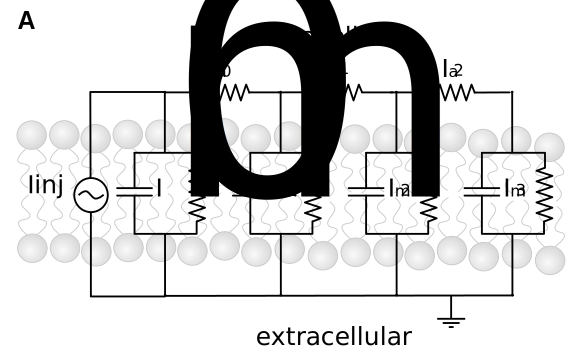
\includegraphics[width=.4\textwidth]{Figures/LFP/cable_equiv_circuit.png}
\includegraphics[width=.4\textwidth]{Figures/LFP/intrinsic_dend_filt.pdf}
\end{center}
\caption{\textbf{Intrinsic dendritic filtering.}
Illustration of the LFP at a snapshot in time in response 
to a sinusoidal synapse with different frequencies to a 
dendritic stick.
}
\label{LFP:fig:intrinsic_dendritic_filt}
\end{figure}


\subsection{\red{TVN:Effect of spikes on the LFP}}
\tvnnote{Hadde vært fint å gå litt ordentlig igjennom dette, men vi får se.}
Typically assumed to not be super important. A lot of the spikes are removed by low-pass filter (but see also Fig.~XX).
Amplitude of LFP grows with population size, but spikes are only visible ~30 µm away from cell. Observed that LFP fluctuations are much larger, and has a different time course.
\citeasnoun**{Reimann2013} says it is important. Probably is important for hippocampal sharp wave ripples \cite**{Schomburg2012, Luo2018}.
\citeasnoun**{Haider2016} says it is synapses.
Can definitely be expected to contribute somewhat to LFP PSDs.


\subsection{\red{TVN: Effect of subthreshold active conductances}}
Since the LFP is thought to mainly originate from large numbers of synaptic inputs and the resulting return currents, it is reasonable to expect that any ion channel on the cellular membrane that might affect the transmembrane currents, would also affect the LFP. Note that most ion channels are closed at the cells resting potential, and only becomes active during spiking.

\subsection{\red{TVN: Other approaches}}
\begin{itemize}
\item "Magic" simple formula \cite**{Mazzoni2015}
\item Kernel trick \cite**{Hagen2015, Skaar2020}
\end{itemize}

\subsection{\red{TBV:Population LFPs}}
\begin{itemize}
\item Full simulations \cite**{Linden2011,Leski2013}
\item Analytical results~\cite**{Einevoll2013a}
\item Active dendrites \cite**{Ness2018}
\item Effect of correlations
\end{itemize}

\subsection{\red{TBV:Effect of synaptic correlations}}
\begin{figure}[!ht]
\begin{center}
\includegraphics[width=1.\textwidth]{Figures/LFP/LFP_effect_correlation_illustration.png}
\end{center}
\caption{\textbf{Illustration of why correlation in synaptic input boosts LFP.}
Basically, it is just because PSD is squared, and variability increase sum of squares: $(1+3) = (2 +2)$, but $(1^2 + 3^2) > (2^2 + 2^2)$
}
\label{LFP:fig:correlation_boost}
\end{figure}



\section{\orange{GTE: Example: How local is the  local field potential?}}
\label{LFP:sec:how-local-is-the-local-field-potential}

The recording of LFPs has a long history in neuroscience. Therefore maybe it is surprising that the question 
`How local is the local field potential' is still debated. How many neurons contribute to the LFP 
recorded by an electric contact? Alternatively, what is the typical radius of the volume surrounding the contact containing
the neurons generating (almost) all of the recorded LFP,  referred to as the \index{spatial reach}? 
Experimental answers to this question have been conflicting, giving estimates for the spatial reach spanning from
a few hundred micrometers~\cite**{Katzner2009,Xing2009} to several millimetres~\cite**{Kreiman2006} or more~\cite**{Kajikawa2011}.
Modelling has revealed that these experimental observations can be reconciled, the key finding being that the spatial reach depends strongly
on how synchronous the synaptic inputs driving the LFP-generating neurons are~\cite**{Linden2011}.

%In \citeasnoun**{Linden2011} it was found that the spatial
%reach depends strongly on how synchronous the synaptic inputs driving the LFP-generating neurons are, see 
%Box~\ref{mm:box:how-local-is-the-local-field-potential}. When the synaptic inputs
%impinging on the population are asynchronous, that is, \firstterm{uncorrelated}, the spatial reach can be as low as hundred micrometers. However, when the synaptic inputs are synchronous manner, that is, \firstterm{correlated}, the spatial reach can be millimetres and even centimeters. 

In \citeasnoun**{Linden2011} this question was addressed by calculationg the spatial size of the pool of neurons 
contributing to the LFP recorded by an electrode. The model used to explore this question
is shown in panel (a) in Figure~\ref{LFP:fig:how-local}.
Here a population of identical pyramidal neurons receiving synaptic inputs is positioned
with circular symmetry in a disc around the recording electrode. The LFP contributions from the individual neurons 
$\phi_i(t)$ sum up to give the total population LFP  $\phi(t)$ (panel b).

%%%%%%%%%%
% Figure: LFP - how local is the local field potential 
%%%%%%%%%%
%\begin{cnfigure}{Figures/mm/how-local-is-the-LFP-w90-r150}
\begin{figure}
\begin{center}
\includegraphics{Figures/LFP/LFP-how-local-is-the-LFP-w90-r150}
\end{center}
\caption[]{Illustration of modelling approach used to explore the question
about the extent of the local field potential.
\gen{The "monopole" part of the figure will not be included.}
\gen{Figure and caption to be updated.}
}
\label{LFP:fig:how-local}
%\figpermOurs
\end{figure}
%%%%%%%%%%%%%%%%%%
  
This total population LFP signal can be computed by using 
Equation~\ref{XX:equation:Ve-multi-compartment} to first compute the signal contribution from each neuron and 
then sum up all the single-neuron contributions to get the compound LFP from the entire population of neurons.
With increasing radius $R$ of the population, more and more neurons will contribute to the compound LFP $\phi(t)$,
and the amplitude $\sigma(R)$ (Figure~\ref{LFP:fig:how-local}b) is thus expected to increase with
$R$. On the other hand the contribution to the compound signal from a single neuron decreases with distance 
as seen in Section~\ref{XX:sec:LFP-single-neurons}, and so intuitively one could expect that $\sigma(R)$ approaches
a constant value $\sigma_\infty$ as the population size $R$ increases. One can then define the spatial reach as the radius for which
the compound LFP has reached a certain fraction $\alpha$ (for example $\alpha$=0.95 as in \citeasnoun**{Linden2011}) of this limiting value $\sigma_\infty$. 

However, it is not clear at the outset that $\sigma(R)$ converges towards a fixed value as $R$ increases and that
a spatial reach defined in this way exists. It turns out that a finite spatial reach is obtained under some conditions, but not all.
We next consider a simple qualitative model that illuminates what factors determine $\sigma(R)$ and when the conditions for
which it converges to a finite value as $R$ increases. 

\subsection{\orange{GTE: Qualitative model}}
Two factors are expected to be key in determining how the compound population LFP $\sigma(R)$ increases with $R$:
(i) how sharply the single-neuron contribution, that is, the \index{shape function} $f(r)$, decays with distance from the neurons, and (ii) the number
density $N(r)$ of neurons positioned in a ring of radius $r$ around the electrode. Here we are interested in the compound LFP for large values of
$R$, and for this only the behavior of the shape function $f(r)$ far away from the neuron is of interest. For such large distances, the far-field dipole approximation
can be assumed, that is, $f(r) \propto 1/r^2$ (Figure~\ref{LFP:fig:how-local}c). 
The number of neurons within each ring will be proportional to the circumference $2\pi r$
of the ring, and $N(r)$ will thus be proportional to $r$ (panel d).

A third key factor is the level of \index{correlations} between the single-neuron contributions to the compound LFP. 

\subsubsection{Uncorrelated single-neuron LFPs}
%\paragraph{Uncorrelated single-neuron LFPs}
In a situation
where the neurons in the population each receive synaptic inputs at completely random times, the contributions will be \index{uncorrelated}, and
there will be strong cancellations of the individual LFP contributions. In this case, the amplitude of the compound signal  $\sigma(R)$ will not be proportional 
to the number of individual sources. However, the variance of the compound LFP, that is, the square of  $\sigma(R)$, will be
given as the sum of the variances of the individual single-neuron contributions. 
(This is analogous to the situation with a so-called random walker where
the variance, that is, square, of the displacement of the walker after $N$ random kicks is proportional to $N$, see, for example, \citeasnoun[Ch. X]{nelson2008}.)

In this case one expects \cite**{Linden2011}
%%%
\begin{equation}
\sigma_\text{u}(R)^2 \propto \sum_i \sigma_i^2 \propto \sum_i f(r_i)^2
\label{LFP:equation:sigmaR2-uncorrelated-sum}
\end{equation}
%%%
Here $\sigma_i$ represents the amplitude of the LFP contribution from the single 
neuron $i$ (Figure~\ref{LFP:fig:how-local}b). This contribution is assumed to 
be proportional to the shape function $f(r_i)$ where $r_i$ is the distance from neuron $i$ to the recording electrode.  
We have further added the subscript `u' to denote that this formula applies to the case of uncorrelated single-neuron LFP contributions.

With many neurons contributing to the compound LFP, we can approximate the sum in Equation~\ref{LFP:equation:sigmaR2-uncorrelated-sum}
with the integral  
%%%
\begin{equation}
\sigma_\text{u}(R)^2 \propto \int_0^R N(r) f(r)^2 dr 
\label{LFP:equation:sigmaR2-uncorrelated-integral}
\end{equation}
%%%
The present focus is on the contribution from the distant neurons where the far-field limit of $f(r)$ applies, that is, where $f(r) \propto 1/r^2$.
For the contributions from these neurons we can approximate the integral in Equation~\ref{LFP:equation:sigmaR2-uncorrelated-integral}
with 
%%%
\begin{equation}
\sigma_\text{u}(R)^2 \sim \int_{R_x}^R N(r) \left(\frac{1}{r^2}\right)^2 dr \propto \int_{R_x}^R \frac{1}{r^3} dr
\propto \frac{1}{R_x^2}-\frac{1}{R^2}
\label{LFP:equation:sigmaR2-uncorrelated-integral-2}
\end{equation}
%%%
Here we have for convenience introduced a lower cut-off radius $R_x$ in the integral to remove the unphysical divergence that would appear by
assuming the far-field relationship $f(r)\sim 1/r^2$ for distances $r$ approaching zero.

The key observation from Equation~\ref{LFP:equation:sigmaR2-uncorrelated-integral-2} is that the variance $\sigma_\text{u}(R)^2$ 
will approach a fixed finite value $\sigma_\infty$ as $R \rightarrow \infty$ (since $1/R^2 \rightarrow 0$ in this limit), Figure~\ref{LFP:fig:how-local}d.
This in turn implies that a spatial reach corresponding to the value of $R$ for which $\sigma_\text{u}(R)=\alpha \sigma_\infty$ can be found.
In the quantitative modelling below, we will see that this spatial reach roughly corresponds to the lateral extension of the dendritic bush, that is, a few hundred micrometers or so when a value of $\alpha$ close to unity is chosen.

\subsubsection{Correlated single-neuron LFPs}
%\paragraph{Correlated single-neuron LFPs}

For fully correlated synaptic inputs onto the neurons, the single-neuron LFP contributions to the compound population LFP will overlap in time.
Further, if the different synaptic inputs have similar spatial positions on the receiving neurons, for example, all placed on the apical dendrites,  there will be little cancellation of their contributions of the single-neuron LFP contributions. 
This is akin to constructive interference in wave physics when, for example, water waves from several sources are added to give interference patterns and a summation of wave crests from the individual wave sources sum up to give a large compound wave.

In this case the compound LFP can be 
approximated by simply summing the individual amplitude contributions. Formulated as an integral, this gives
%%%
\begin{equation}
\sigma_\text{c}(R) \propto \int_0^R N(r) f(r) dr 
\label{LFP:equation:sigmaR-correlated-integral}
\end{equation}
%%%
When we now insert $N(r) \sim r$ and $f(r) \sim 1/r^2$, we find that the contributions from the neurons
positioned outside a radial distance $R_x$ from the electrode is given by
%%%
\begin{equation}
\sigma_\text{c}(R) \propto \int_{R_x}^R r \frac{1}{r^2} dr =  \int_{R_x}^R \frac{1}{r} dr = \ln \frac{R}{R_x} 
\label{LFP:equation:sigmaR-correlated-integral-2}
\end{equation}
%%%
The key observation here is that the amplitude $\sigma (R) \rightarrow \infty$ when $R \rightarrow \infty$.
Thus unlike for the uncorrelated case, the LFP amplitude increases without bound as the population size $R$ increases, 
and the compound LFP signal thus has an `infinite' spatial reach.

The question of whether the spatial reach of the LFP signal is finite or infinite has some resemblance to  
the ancient question of why the night sky is dark given the numerous stars in the universe. This so-called
Olbers' paradox and the link to the spatial-reach question is described in Box XX.


\subsection{\red{GTE: Box:  Why is the night sky dark? Olbers' paradox}}
\gen{Was a Box in chapter in Sterratt}
%%%%%%%%%%
% Box: Why is the night sky dark? Olbers' paradox
%%%%%%%%%%
%\begin{boxfloat}{Olbers' paradox and population LFPs}
%  \label{LFP:box:Olbers}
%
\begin{center}
\includegraphics{Figures/LFP/LFP-night-sky-w90-r150}
\end{center}
\vspace*{6pt}
%
Why is the night sky dark? An interesting historical paradox from astronomy, known as Olbers' paradox~\cite**{Harrison1989}, has some analogies with the question of summation of LFP signals from many neurons. The question is why the night sky is dark given the following:
(i) the light intensity from a single star falls off as $1/r^2$, (ii) in a homogeneous universe the number of stars in a spherical shell of a certain thickness around the Earth should increase as $r^2$. According to this the contribution from each such shell of stars to the illumination on Earth should thus be independent of the distance $r$. With an infinite universe there will be an infinite number of shells and thus an infinite light intensity on Earth! This paradox is resolved if one takes into account modern knowledge that the universe is not infinitely old and the speed of light is finite so that there are no contributing stars for shells at distances of 14 billion light years or more away. This summation of light from numerous starts is analogous to the summation of LFP from numerous neurons in the surrounding brain. A difference is that while neuronal LFPs are essentially dipoles, the stars are monopole light sources. Also the geometry is different (three-dimensional shells for stars, two-dimensional rings for neurons). The outcome is that while a finite brain is not required for a finite LFP, a finite universe is indeed required to resolve Olbers' paradox.
\gen{This text is copied directly from a book chapter we wrote (Einevoll2013a) and should be modified to avoid self-duplication.}
%\end{boxfloat}
%%%

\subsection{\orange{GTE: Quantitative model}}

The results from the qualitative modelling above demonstrates that the size of the compound LFP 
from a population of neurons receiving synaptic inputs, depend critically on the level of 
correlation in the synaptic inputs. To obtain a more
precise picture of how the compound LFP grows with population size, we here investigate a 
corresponding quantitative model where the single-neuron contributions $f(r)$ is specified in detail.

Figure~\ref{LFP:fig:how-local-shape-function} shows results for how the LFP signal decays with distance from the soma of neurons when moving sideways from the depth of the neuronal somas
(similar to  Figure~\ref{LFP:fig:distance-decay}c). As seen in Figure~\ref{LFP:fig:how-local-shape-function}b, the decay of the LFP signal with lateral distance follows a very standardised form. For all three neuronal morphologies considered the single-neuron LFP signal decays roughly as $1/\sqrt{r}$ close to the neuron and as $1/r^2$ (as expected for a current dipole) far away from the neuron. 

This suggests the following general form for the shape function $f(r)$ 
(Figure~\ref{LFP:fig:how-local-shape-function}c,d):
%
\begin{equation}
  f(r)=
  \begin{cases}
    f_0 & r< r_\varepsilon \\
    f_0\,\left(r_\varepsilon/r\right)^{1/2} &  r_\varepsilon \le r < r_* \\
    f_0\,\left(r_\varepsilon/r_*\right)^{1/2}\,\left(r_*/r\right)^{2}  & r \ge r_* \;\;,
  \end{cases}
\label{LFP:equation:f-power-law}
\end{equation}
%
Here $r_*$ is the radial distance at which the amplitude decay changes from $1/\sqrt{r}$ to $1/r^2$.
From Figure~\ref{LFP:fig:how-local-shape-function}b we see that $r_*$ is about 100~micrometers for all the presently considered neurons. We have also introduced a lower cut-off $r_\varepsilon$ under 
which the signal is assumed to be constant rather than diverging as $1/\sqrt{r}$. This cut-off reflects the finite size of the neuronal somas so $r_\varepsilon$ could be about 10 micrometers or so. 

For the example in Figure~\ref{LFP:fig:how-local-shape-function} where synaptic inputs are evenly spread across the dendritic membranes, the parameter $r_*$ can be assumed to be roughly the same for the three example neurons. This is not so for the parameter $f_0$ describing the overall amplitude of the signal, however. This parameter will in general depend not only on the neuronal morphology, but in particular on the number and strength of synaptic inputs ~\cite**{Linden2010,Linden2011,Einevoll2013a}.

%%%%%%%%%%
% Figure: LFP - how local - shape - function
%%%%%%%%%%
%\begin{cnfigure}{Figures/mm/EP-how-local-shape-function-w100-r150}
\begin{figure}
\begin{center}
\includegraphics{Figures/LFP/LFP-how-local-shape-function-w100-r150}
\end{center}
\caption[]{Shape function
\gen{Figure and caption to be updated.Change $r_*$ to 0.1 mm?
Mention uncorrelated inputs to make figure. Mention that $r_*$ is larger for apical inputs
onto L5 neurons, cf. Figure in Linden 2011.}
}
\label{LFP:fig:how-local-shape-function}
%\figpermOurs
\end{figure}
%%%%%%%%%%%%%%%%%%


\subsubsection{Uncorrelated single-neuron LFPs}
%\paragraph{Uncorrelated single-neuron LFPs}

For the case with uncorrelated single-neuron LFPs, the integral in Equation~\ref{LFP:equation:sigmaR2-uncorrelated-integral} for the variance of the compound LFP signal can now
be written as 
%%%
\begin{equation}
\sigma_\text{u}(R)^2  = \int_0^R N(r)  f(r)^2 dr  = \rho \int_0^R 2 \pi r  f(r)^2 dr 
\label{LFP:equation:sigmaR2-uncorrelated-quantitative}
\end{equation}
%%%
where we have used $N(r)dr=2\pi r \rho dr$ with $\rho$ being the area density of neurons
contributing to the LFP. Insertion of $f(r)$ from 
Equation~\ref{LFP:fig:how-local-shape-function} then gives after some algebra
%%%
\begin{equation}
  \sigma_\text{u}(R)^2= 
  \begin{cases}
    f_0^2 \, \rho \, \pi R^2                   &   R \le r_\varepsilon   \;\;,\\
    f_0^2 \, \rho \, \pi r_\varepsilon (2 R - r_\varepsilon)  &   r_\varepsilon \le R \le r_*  \;\;,\\
    f_0^2 \, \rho \, \pi r_\varepsilon (3 r_* - r_\varepsilon  - r_\star^3/R^2)  & R \ge r_* \;\;,
  \end{cases}
\label{LFP:equation:sigmaR2-uncorrelated-quantitative-2}  
\end{equation}
%%%
The corresponding formula for the LFP amplitude $\sigma_\text{u}(R)$, found by taking the 
square root of the expressions in Equation~\ref{LFP:equation:sigmaR2-uncorrelated-quantitative-2},
is illustrated in Figure~\ref{LFP:fig:how-local-center-of-population}(a).  
\gen{ Unsure whether to give the formula for $\sigma_\text{u}(R)$ instead of $\sigma_\text{u}(R)^2$.}

%
%%%%%%%%%%
% Figure: LFP - how local - center of population
%%%%%%%%%%
%\begin{cnfigure}{Figures/mm/EP-how-local-center-of-population-w100-r150}
\begin{figure}
\begin{center}
\includegraphics{Figures/LFP/LFP-how-local-center-of-population-w100-r150}
\end{center}
\caption[]{Population LFP at center of population for uncorrelated neurons.
\gen{Figure and caption to be updated. 
Panel (a) must include region smaller than $r_\varepsilon$. Explain dashed lines.
Change $r_*$ to 0.1 mm? Make figure with real numbers (millivolts) on the y-axis.}
}
\label{LFP:fig:how-local-center-of-population}
%\figpermOurs
\end{figure}
%%%%%%%%%%%%%%%%%%
%

A first observation from the figure is that $\sigma_\text{u}(R)$ seems to approach a finite
value as $R \rightarrow \infty$, and from the formula in Equation~\ref{LFP:equation:sigmaR2-uncorrelated-quantitative-2}  
we see that this value is given by $\sigma_\infty = f_0^2 \, \rho \, \pi r_\varepsilon (3 r_* - r_\varepsilon)$. For the parameter values used in Figure~\ref{LFP:fig:how-local-center-of-population} this gives  
$\sigma_\infty=$XX~millivolts. 

The analytical formulae in Equation~\ref{LFP:equation:sigmaR2-uncorrelated-quantitative-2} 
further suggest a new definition of the spatial reach $R_\text{reach}$, that is, $R_\text{reach}$ 
can be set to be the distance from the electrode at which the 
intermediate-$R$ ($r_\varepsilon \le R \le r_*$) and the 
infinite-$R$ ($R \rightarrow \infty$) formulae intersect~\cite**{Einevoll2013a}, see 
Figure~\ref{LFP:fig:how-local-center-of-population}a. For this particular value of $R$ we have 
$2R_\text{reach}-r_\varepsilon=3 r_* - r_\varepsilon$, that is, $R_\text{reach} =1.5 r_*$. 

Insertion of $R=R_\text{reach}=1.5 r_*$ into Equation~\ref{LFP:equation:sigmaR2-uncorrelated-quantitative-2} 
gives that $\sigma (R_\text{reach})=\sqrt{23/27}\sigma_\infty \simeq 0.92 \sigma_\infty$ independent of the value of $r_*$ (as long as $r_\varepsilon \ll r_*$ like it is in the present numerical example). Thus for the present case with uncorrelated neuronal sources, the model implies that 92\% of the LFP amplitude recorded by an electrode in the centre of a disc-like population 
stems from neurons closer than $R_\text{reach}=1.5~r_*$. For the numerical values
used in Figure~\ref{LFP:fig:how-local-center-of-population}a,
this corresponds to $R_\text{reach}$=0.15~mm. 
Note that this result pertains to the situation where the electrode is at the same depth level as the neuronal somas. But the same reasoning and modelling can equally be used for the case where the neuronal somas are above or below the recording electrode, see~\citeasnoun**{Einevoll2013a}.

We can now ask the question of how many neurons contribute to the recorded LFP. To get a rough idea, we can estimate the number of neurons with somas contained within a sphere of radius $R_\text{reach}$
around the electrode. With a neuron density of, for example, $\rho_\text{neuron}$=50000 neurons per mm$^3$ which is typical for grey matter in 
cortex~\gen{REF:Beaulieu 1993}, we find that this sphere will contain $N_\text{neuron}=4 \pi R_\text{reach}^3 \rho_\text{neuron}/3$=\gex{XX}~neurons.


\subsubsection{Correlated single-neuron LFPs}
%\paragraph{Correlated single-neuron LFPs}

For the case with correlated single-neuron LFPs, insertion of the shape function $f(r)$ from 
Equation~\ref{LFP:equation:sigmaR2-uncorrelated-quantitative-2}  into the integral
%%%
\begin{equation}
\sigma_\text{c}(R)  = \int_0^R N(r)  f(r) dr  = \rho \int_0^R 2 \pi r  f(r) dr 
\label{LFP:equation:sigmaR2-correlated-quantitative}
\end{equation}
%%%
gives
%%%
\begin{equation}
  \sigma_\text{c}(R) =
  \begin{cases}
    f_0^2 \, \rho^2 \, \pi^2 R^4                   &   R \le r_\varepsilon   \;\;,\\
    f_0^2 \, \rho^2 \frac{1}{9} \pi^2 \left( r_\varepsilon^2 - 4 r_\varepsilon^{1/2} R^{3/2} \right)^2 \;\;, &   r_\varepsilon \le R \le r_* \\
    f_0^2 \, \rho^2 \frac{1}{9} \pi ^2 r_{\varepsilon } \left(r_{\varepsilon }^{3/2}-\left(4+6 \ln\left(R/r_*\right)\right) r_*^{3/2}\right)^2
  & R \ge r_* \;\;,
  \end{cases} 
  \label{LFP:equation:sigmaR2-correlated-quantitative-2}  
\end{equation}
%%%
In this case the compound population LFP amplitude $\sigma_\text{c}(R)$ does not approach a finite fixed value $\sigma_\infty$ as $R \rightarrow \infty$, rather the LFP amplitude
displays logarithmic divergence, i.e., $\sigma (R) \sim \ln(R/r_*)^2$ in this limit, see Figure~\ref{LFP:fig:how-local-center-of-population}b.
Thus the LFP would in principle be infinite if the electrode was surrounded by an infinite sea of correlated neuronal LFP sources. Of course, this unbounded amplification of the LFP amplitude will never occur  
due to the necessarily finite size of pools of correlated neuronal LFP sources in the cortex. (In fact, this is also an explanation for 
why the night sky is dark and not light due to the illumination from all the stars surrounding us, see  Box \gex{Olbers}.
%~\ref{LFP:box:Olbers}.)

For correlated LFP sources, the model predicts that the spatial reach in practice will be set by the size of the pool of neurons receiving correlated synaptic inputs surrounding the electrode, see \citeasnoun[Figure~5]{Linden2011}. This may explain why experimental estimates of the spatial reach has varied so widely, from a few hundred micrometers to centimetres \gen{Kreiman2006, Liu and Newsome2006, Berens et al 2008a, Katzner2009, Xing et al. 2009}.

The above formulae for $\sigma_\text{c}(R)$ for the population LFP represent the two extreme cases where either the single-neuron
LFPs are completely uncorrelated (Equation~\ref{LFP:equation:sigmaR2-uncorrelated-quantitative-2}) or completely correlated 
(Equation~\ref{LFP:equation:sigmaR2-correlated-quantitative-2}). In reality one would expect the situation to be somewhere in between, that is,
the single-neuron LFPs will be partially correlated. However, a corresponding formula for $\sigma_\text{c}(R)$ for arbitrarily levels of correlations can also be found, see Box~\ref{LFP:box:population-LFP-general}. 

\gen{GTE: Note that the boost of LFPs requires asymmetric input.}
 
 
 
%%%%%%%%%%
% Box: General expression for compound LFP
%%%%%%%%%%
\subsection{\red{GTE: Box: General expression for population LFP}}
\gen{This was a box in Sterratt chapter}
%\begin{boxfloat}{General expression for population LFP}
%  \label{LFP:box:population-LFP-general}
The formulae in Equations~\ref{LFP:equation:sigmaR2-uncorrelated-quantitative-2} 
and~\ref{LFP:equation:sigmaR2-correlated-quantitative-2} predict how the amplitude  $\sigma$ 
for the population LFP will depend on the population radius $R$ for the cases of uncorrelated or completely correlated
single-neuron LFPs, respectively. However, an analogous formula for the intermediate case with partially correlated single-neuron LFPs, can
also be derived.

Following \citeasnoun**{Linden2011} we assume the single-neuron LFP contribution $\phi_i(t)$ from a neuron $i$ to be a product of a 
temporal part $\xi_i(t)$ and a spatial part $f(r_i)$ where $r_i$ is the distance between the neuron and the electrode:
%%%
\begin{equation}  
\phi_i(t)= \xi_i(t) f(r_i)
\label{LFP:box:equation:phii}
\end{equation}
%%%
Further, $f(r_i)$ is assumed to be given by the shape function in 
Equation~\ref{LFP:equation:f-power-law}, and $\xi_i(t)$ is a time-dependent function with a mean value of zero and a unit variance, that is,
$\langle \xi_i(t)^2 \rangle$=1. Here $\langle \cdot \rangle$ represents averaging over time.

We now introduce the \index{pair-wise correlation} 
%%%
\begin{equation}
c_\phi=\langle \xi_i(t) \xi_j(t)\rangle\, ,\;\; i \neq j
\label{LFP:box:equation:phii}
\end{equation}
%%%
and assume that is has the same value for all pairs $i \neq j$. With this notation,  
\emph{uncorrelated} single-neuron LFP sources corresponds to $c_\phi=0$ and 
completely \emph{correlated} single-neuron LFP sources corresponds to $c_\phi=1$.

With the general applicable expression
%%%
\begin{equation}
\langle \phi_i(t) \phi_j(t) \rangle= c_\phi f(r_i) f(r_j)\, , \;\; i \neq j
\label{LFP:box:equation:phii-phij}
\end{equation}
%%%
it was shown in \citeasnoun**{Linden2011} that the population LFP amplitude is given as
%%%
\begin{equation}
  \sigma(R)=\sqrt{(1-c_\phi) \sigma_\text{u}(R)^2 +  c_\phi \sigma_\text{c}(R)^2}\;\;.
  \label{LFP:box:equation:sigmaR}
\end{equation}
%%%
where $\sigma_\text{u}(R)$ is given by the expression in Equation~\ref{LFP:equation:sigmaR2-uncorrelated-quantitative-2} and
 $\sigma_\text{c}(R)$ by the expression in Equation~\ref{LFP:equation:sigmaR2-correlated-quantitative-2}.

A notable difference between the uncorrelated $\sigma_\text{u}(R)$ and fully correlated expressions $\sigma_\text{c}(R)$ is that 
the former is proportional to the square root of the neuron density $\rho$ while the latter is proportional the neuron density itself.
Thus, all else equal, the relative contribution from the correlated sources will be larger with larger neuronal densities. 
%\end{boxfloat}
%%%


\subsection{\orange{GTE: How sharply does the LFP decay outside a population of neurons?}}

Another way to phrase the question of how local the LFP is, is to measure how sharply the LFP decays outside a neuronal population receiving synaptic inputs.
This can be explored with our quantitative model by computing how the recorded LFP will decay when the recording electrode is moved away from the center of 
the population. We label this distance $X$ and assume, as above, a circularly symmetric neuronal population. 

\subsubsection{Uncorrelated sources} 
For the case with uncorrelated single-neuron LFP contributions, the integral in Equation~\ref{LFP:equation:sigmaR2-uncorrelated-quantitative}
giving the amplitude of the population LFP signal is now replaced by~\cite**{Einevoll2013a} 
%%%
\begin{equation}
\sigma_\text{u}(R,X)^2 =  \rho \iint_{\{|\vec{r}|\le R\}}\, f(|\vec{r}-\vec{X}|)^2  \, dA 
\label{LFP:equation:sigmaR2-X-uncorrelated-quantitative-1}
\end{equation}
%%%
Here the integral goes over the disc area of the population, and $\vec{X}$ is the vector $X\,\vec{e}_x$, 
with $\vec{e}_x$ being a unit vector in the $x$-direction. Note that for the special case $X$=0, that is, when
the electrode is positioned in the center of the population, the integral reduces to 
Equation~\ref{LFP:equation:sigmaR2-uncorrelated-quantitative} as it should.
Using cylindrical coordinates the area integral in Equation~\ref{LFP:equation:sigmaR2-X-uncorrelated-quantitative-1} 
can be written as
%%%
\begin{equation}
\sigma_\text{u}(R,X)^2 
%& = &  \rho \iint_{\{|\vec{r}|\le R\}}\, f(|\vec{r}-\vec{X}|)^2 \, dA \\
           =  \rho \int_0^{2\pi} d\theta \int_0^R dr \, r f \left( \sqrt{(X-r\cos\theta)^2+(r\sin\theta)^2} \right)^2\;\;, 
\label{LFP:equation:sigmaR2-X-uncorrelated-quantitative}
\end{equation}
%%%
for which solutions in general must be found numerically. 
\gen{How should this 2D integral be displayed? dr at the end?}

\subsubsection{Correlated sources} 
Likewise, for the case of completely correlated single-neuron LFP contributions, 
the integral in Equation~\ref{LFP:equation:sigmaR2-correlated-quantitative} becomes
%%% 
\begin{eqnarray}
  \sigma_\text{c}(R,X) & = &  \rho \iint_{\{|\vec{r}|\le R\}} \, f(|\vec{r}-\vec{X}|)   \, dA \nonumber \\
           & = &  \rho \int_0^{2\pi} d\theta \int_0^R dr \, r f \left( \sqrt{(X-r\cos\theta)^2+(r\sin\theta)^2}\right) \;.
\label{LFP:equation:sigmaR2-X-correlated-quantitative}           
\end{eqnarray}
%%%
\gen{GTE: Doublecheck formulae}

For the intermediate case with some, but not complete correlation of the single-neuron LFPs $(0 < c_\phi < 1)$ 
(Equation~\ref{LFP:box:equation:phii-phij} in Box~\ref{LFP:box:population-LFP-general}), the population amplitude
$\sigma(R,X)$ is found by replacing $\sigma_\text{u}(R)$ and  $\sigma_\text{c}(R)$  with the functions
$\sigma_\text{u}(R,X)$ and  $\sigma_\text{c}(R,X)$, respectively, in 
Equation~\ref{LFP:box:equation:sigmaR} in Box~\ref{LFP:box:population-LFP-general}.

In Figure~\ref{LFP:fig:how-local-outside-population-center} some example results for
$\sigma_\text{u}(R,X)$ (panel a) and  $\sigma_\text{c}(R,X)$ (panel b) are shown. 
Outside a large disc-like population with radius $R=1$~millimetre we observe that in both cases
the LFP amplitude decays sharply outside the population edge. The decay length is set by the value
of $r_*$ as is demonstrated when comparing results using  $r_*=0.15$~millimetres and  $r_*=0.30$~millimetres, 
respectively. For a small population diameter ($R=0.2$~millimetre) the dependence on the lateral electrode position $X$ is seen to be
less sharp, demonstrating that a sharp decay requires $r_* \ll R$.

%%%%%%%%%%
% Figure: LFP - how local - outside population center
%%%%%%%%%%
%\begin{cnfigure}{Figures/mm/EP-how-local-outside-population-center-w100-r150}
\begin{figure}
\begin{center}
\includegraphics{Figures/LFP/LFP-how-local-outside-population-center-w100-r150}
\end{center}
\caption[]{Population LFP outside center of population. 
Left: Uncorrelated. Right: Correlated.
\gen{Figure and caption to be updated.
Maybe illustrate set up and "half-plane" argument.}
}
\label{LFP:fig:how-local-outside-population-center}
%\figpermOurs
\end{figure}
%%%%%%%%%%%%%%%%%%

When comparing the population LFPs for the uncorrelated and fully correlated cases in
Figure~\ref{LFP:fig:how-local-outside-population-center} we observe that 
relative to the amplitude recorded in the population center, the LFP amplitude at the 
population edge $\sigma(R,R)$ is larger for uncorrelated cases than the correlated cases.
This can be qualitatively understood by considering $\sigma(R,R)$ in the limit $R \rightarrow \infty$ where
being on the edge approaches the situation of being at the edge of an infinitely large half-plane. In this
situation, the recorded variance of the LFP at the center of the population will correspond to being in the middle
of an infinite plane, that is, the sum of the signal variance from two infinitely large half-planes. We thus have
$\sigma_\text{u}(R,0)^2=2\sigma_\text{u}(R,R)^2$, so that  $\sigma_\text{u}(R,R)/\sigma_\text{u}(R,0)=\sqrt{2} \simeq 0.71$. For the case with
$R=1$~millimetre in Figure~\ref{LFP:fig:how-local-outside-population-center}(a) we indeed observe 
$\sigma(R,R)/\sigma(R,0) \sim 0.7$ even though $R/r_*$ (which is the relevant measure) in this case
is only about 10 or so.

For the fully correlated case we find by the same argument that  $\sigma_\text{c}(R,0)=2\sigma_\text{c}(R,R)$ so that
$\sigma_\text{c}$ at the edge should be about half of  $\sigma_\text{c}$ in the population center when 
$R \rightarrow \infty$. And this is indeed close to what is observed for $R=1$~millimetre in 
Figure~\ref{LFP:fig:how-local-outside-population-center}(b). 

Close inspection of the large-$X$ tail of the population-LFP curves in Figure~\ref{LFP:fig:how-local-outside-population-center}
reveals a power law, that is, $\sigma(R,X) \sim 1/X^2$~\cite**[Figure~3.9]{Einevoll2013a}. For sufficiently large values of $X$, that is,
$X \gg R$, inspection of the integral expressions in Equations~\ref{LFP:equation:sigmaR2-X-uncorrelated-quantitative}  
and~\ref{LFP:equation:sigmaR2-X-correlated-quantitative} in fact reveals that in this limit the population LFP will exhibit the 
same large-X power-law behaviour as the single-neuron shape function $f(r)$, see \cite**{Einevoll2013a}.      


\section{\red{TVN/EH: Network LFPs}}
\begin{itemize}
\item Cortical LFPs from single corticothalamic neuron \cite**{Hagen2017}
\item Cortical networks with passive dendrites with hybrid trick \cite**{Hagen2016}
\item Cortical network with active dendrites \cite**{Reimann2013}
\end{itemize}

\section{\red{GTE: Insights from LFP studies}} 

\chapter{TVN/SN: ECoG}
\label{chap:ECoG}
\ghnote{Torbjorn or Solveig will write this chapter?}

\section{\red{TVN/SN: Insights from ECoG studies}} 

\section{EEG}
\label{sec:EEG}
\ghnote{Solveig will write this chapter?}



\subsection{4-sphere model} 
Kjernereferanse: \citep{Naess2017} and Naess et al (in preparation).


\subsection{Insights from EEG studies} 

\chapter{TVN/GH: MEG}
\label{chap:MEG}
\index{MEG}
\ghnote{
Here we must understand the relationship between "impressed currents" and "primary currents" as they are used in the MEG litterature, i.e., in the book Brain Signals. So far, we have MEG only as an application-chapter. Should we have a theory chapter magnetic fields it in Part 1, or will we sneak the theory in here as we go along?}

\sntxt{
I've looked into this matter as part of writing my kappe, and this is my conclusion.

We write the continuity equation as follows:

\begin{equation} \label{eq:MEG:continuity}
{\bf \nabla} {\bf i}_t = C
\end{equation}
based on \citep{Gratiy2017}.

${\bf i}_\mathrm{t}$ is here the tissue current density resulting from the current source density $C$. All "impressed currents" (i.e. transmembrane currents), are in our case included in $C$.

Next, we write Ohm's law this way:

\begin{equation}\label{eq:MEG:ohm_1}
{\bf i}_\mathrm{t} = \sigma {\bf E}.
\end{equation}

Inserting Equation \eqref{eq:MEG:ohm_1} into Equation \eqref{eq:MEG:continuity}, applying ${\bf E} = -{bf \nabla} V$, gives the Poisson equation:

\begin{equation}\label{eq:MEG:poisson1}
{\bf \nabla} \cdot (\sigma {\bf \nabla} V) = -C.
\end{equation}



%The quasistatic version of Maxwell's fourth equation explains how an electric current gives rise to a magnetic field {\bf B}. In the brain, the magnetic permeability $\mu$ is very close to the magnetic permeability in vacuum $\mu_0$ \cite{Hamalainen}, such that:
%
%\begin{equation}\label{eq:MW4_qs_2}
%\nabla \times {\bf B} = \mu_0 {\bf i}
%\end{equation}
%
%In order to derive an expression for ${\bf B}$ (as in \cite{Griffiths1999}), we start by defining the vector potential ${\bf A}$
%
%\begin{equation}\label{eq:defA}
%{\bf B} = {\bf \nabla} \times {\bf A},
%\end{equation}
%
%with zero divergence ${\bf \nabla \cdot A} = 0$. Inserting \eqref{eq:defA} into \eqref{eq:MW4_qs_2}, we see that:
%
%\begin{equation*}
%\nabla \times {\bf B} = \nabla \times ({\bf \nabla} \times {\bf A})
%					 = {\bf \nabla} ({\bf \nabla} \cdot {\bf A})
%					    - {\bf \nabla}^2 {\bf A}
%					 = \mu_0 {\bf i}
%\end{equation*}
%
%Since we have defined ${\bf \nabla} \cdot {\bf A} = 0$ (see \cite{Griffiths1999}), we end up with the Poisson equation:
%
%\begin{equation}\label{eq:poisson_A}
%{\bf \nabla}^2 {\bf A} = -\mu_0 {\bf i},
%\end{equation}
%
%which can be solved in the same way as \sntxt{the electric field Poisson equation}, assuming that {\bf i} goes to zero at infinity:
%
%\begin{equation}\label{eq:A}
%{\bf A}({\bf r}) = \frac{\mu_0}{4\pi} \int \frac{{\bf i}({\bf r}')}{|{\bf r} - {\bf r}'|} dV'.
%\end{equation}
%
%We now obtain the following expression for the magnetic field:
%
%\begin{equation}\label{eq:B}
%{\bf B}({\bf r}) = \frac{\mu_0}{4\pi} \int {\bf \nabla} \times \frac{ {\bf i}({\bf r}')}{|{\bf r} - {\bf r}'|} dV'.
%\end{equation}
%
%Using the identity
%
%${\bf i} = {\bf i}_p - \sigma {\bf \nabla} V$



}

\section{\red{TVN: Insights from MEG studies} }
The human being is essentially just a very weak electromagnet. 
\section{TVN: Electrical stimulation}
\label{sec:Stim}
\tvnnote{Torbjørn skriver dette}

\subsection{\red{TVN TO WRITE THIS}}
\begin{itemize}
\item General principle with illustration figure?
\item Only change in external potential matters, emphasizing importance of distance to electrode and electrode size.
\item Only change along neurites matter, not across membrane (electric field across membrane is already immense).
\item Activation function: Strengths and weaknesses
\item Axon terminals are main targets of action potential initiation, seen both in experiments and simulations.
\item Negative current pulses will depolarize proximal part of cell and hyperpolarize distal part of cell. Opposite for positive current.
\end{itemize}

\begin{figure}[!ht]
\begin{center}
\includegraphics[width=1\textwidth]{Figures/Stim/current_stimulation_example.png}
\end{center}
\caption{\textbf{Illustration of extracellular stimulation (from cortical surface)} 
}
\label{Stim:fig:current_stimulation_example}
\end{figure}

\part{Outlook}
%\include{Ch-ephaptic}
%\section{Schemes for computing EPs from neural activity}
\label{sec:Schemes}
\ghnote{Geir and Torbjorn will write most this. Torbjorn takes care of the LFPy-part, Geir takes care of the other schemes.}
\ghnote{GH: I reorganized this following the logic from the theory part - starting with the VC-stuff.}

There exist several different schemes for computing the extracellular dynamics surrounding active cells, varying in terms of completeness. In this chapter, we summarize the schemes depicted in Fig. \ref{Schemes:fig:schemes}, where they have been classified by whether or not they are (i) self consistent, and whether or not they (ii) account for effects of ion concentration dynamics (Fig. \ref{Schemes:fig:schemes}). By self consistent, we mean that the neuronal and extracellular dynamics are modeled on a unified framework, so that (ephaptic) effects of extracellular variables on the neurodynamics are accounted for. 

\begin{figure}[!ht]
\begin{center}
\includegraphics[width=0.8\textwidth]{Figures/Schemes/schemes.png}
\end{center}
\caption{\textbf{Overview of schemes for computing extracellular dynamics.} The extracellular potential largely originates from neuronal transmembrane currents, illustrated for a simple (two-compartment) neuron, with currents that cross its membrane in the form of a current sink $I_1$ in one compartment, and a current source $I_2$ in the other (green arrows). {\textbf (A)}: HHC+VC: Two-step procedure which (step 1) computes transmembrane neural currents in an independent simulation using Hodgkin-Huxlley-Cable (HHC) formalism, and then (step 2) from these computes the extracellular potential using Volume Conductor (VC) theory. {\textbf (B)}: HHC + KNP: Two-step scheme, which (step 1) computes currents and ion fluxes in an independent simulations based on HHC, and (step 2) from these computes the changes in the extracellular potential and ion concentrations based on an electrodiffusive Kirchhof-Nernst-Planck (KNP) scheme. {\textbf (C)}: EMI (Extracellular-Membrane-Intracellular): Computes neurodynamics and extracellular dynamics on a unified framework, and thus accounts for ephaptic effects. EMI only keeps track of net electrical currents, and assumes ion concentrations to be constant. {\textbf (D)}: PNP or KNP+EMI: Compute electrical potentials and ion concentration dynamics in the intra- and extracellular space on a unified, electrodiffusive framework based on either the Poisson-Nernst-Planck (PNP) set of equations, or a combination of EMI and KNP. 
}
\label{Schemes:fig:schemes}
\end{figure}

The Hodgkin-Huxley-Cable + Volume Conductor (HHC+VC) scheme (Fig. \ref{Schemes:fig:schemes}A) is the standard, two-step scheme that we introduced in Chapters \ref{sec:Neuron}-\ref{sec:Sigma} of this book. Although the HHC+VC scheme is not self-consistent, and does not account for effects of ion concentration dynamics, it is the most "user-friendly" scheme, and is thought to be sufficient for most purposes. For purposes where it is not, one should consider one of the alternative schemes, which account for ion concentration dynamics (Fig. \ref{Schemes:fig:schemes}B), ephaptic effects (Fig. \ref{Schemes:fig:schemes}C) or both (Fig. \ref{Schemes:fig:schemes}D).

When organizing the content of Part 1 of this book, we have mostly followed the principle that we first present the simplest operational model, and then follow up by expanding it to more general cases and discussing the underlying assumptions and details. For the current chapter, we have done things the other way around. We present the complete, self-consistent electrodiffusive schemes first (Section: \ref{sec:Schemes:complete}), to show how the less complete schemes (Sections \ref{sec:Schemes:KNP}-\ref{sec:Schemes:VC}) can be seen as reductions of the former. 
Some readers might want to skip directly to the standard VC-theory based schemes (Section \ref{sec:Schemes:VC}).


%%%%%%%%%%%%%%%%%%%%%%%%%%%%%%%%%%%%%%%%%%%

\subsection{\red{Self-consistent electrodiffusive schemes}}
\label{sec:Schemes:complete}
The transmembrane ionic currents that mediate neurodynamics will in principle cause the intra- and extracellular ion concentrations to change. Under normal circumstances, concentrations tend to change very little, as neurons and glial cells contain numerous homeostatic mechanisms that work continuously to restore baseline concentrations. However, during neuronal hyperactivity, or during several pathological conditions, the homeostatic mechanisms can fail to keep up, and ion concentrations may change over time, both in the intra- and extracellular space  \cite{Dietzel1989, Somjen2001, Frohlich2008, Zandt2015review, Ayata2015}. This will lead to changes in neuronal reversal potentials (cf. eq. \ref{Neuron:eq:revpots}), which in turn will change neuronal firing properties, which has been the topic of several studies (see e.g., \cite{Qian1989, Cressman2009, Oyehaug2009, Zandt2011, Saetra2020}). Changes in extracellular concentrations can also evoke diffusive currents in the extracellular space, which may have an impact on the extracellular potential $\phi$. Then, $\phi$ is not solely a function of cellular transmembrane currents (as predicted from VC theory), but also reflects extracellular diffusion \cite{Halnes2016}. 

To simultaneously account for all concentration effect, we can compute all concentrations and their coupling to the electrical potential by requiring that the Nernst-Planck continuity equation:
\begin{equation}
\frac{\partial c_k}{\partial t} = {\bf \nabla} \cdot \left[{D_k} {\bf \nabla} c_k + \frac{D_k z_k c_k}{\psi} {\bf \nabla} \phi \right].
\label{Schemes:eq:NP}
\end{equation}
should be fulfilled at all points in space. Eq. \ref{Schemes:eq:NP} gives us one equation for each individual ion concentration $c_k$, and to solve the system of equations, we are in need an additional equation for the additional variable, the electrical potential $\phi$, which couples the dynamics of the individual ion species. There are two main approaches to this, the so-called \textit{Poisson-Nernst-Planck (PNP)} framework, or the so-called \textit{electroneutral} framework, both of which we will introduce in the following subsections. 


\subsubsection{\blue{The Poisson-Nernst-Planck (PNP) framework}}
\label{sec:Schemes:PNP}
The physically most detailed approach for defining $\phi$ in the eq. \ref{Schemes:eq:NP}) is to use Poisson's equation from electrostatics:
\begin{equation}
\nabla^2 \phi = -\rho/\epsilon
\label{Schemes:eq:poisson}
\end{equation}
Here $\epsilon$ is the permittivity of the medium, and in the last step, we have expressed the local charge density $\rho$ as a function of the ionic concentrations. 
\begin{equation}
\rho = F\sum_k z_k c_k.
\label{Schemes:eq:PNPrho}
\end{equation}

The PNP equations (eq. \ref{Eldiff:eq:NP} together with eq. \ref{Eldiff:eq:poisson}) can in principle be solved for arbitrary complex geometries using numerical methods, like the Finite Element Method (FEM). 

To apply the PNP scheme poses several challenges. Firstly, one needs to represent the geometry and properties of the cellular membranes. In principle, this could be achieved through having spatially and temporally varying diffusion coefficients $D_k$, and membranes would be characterized with values of $D_k$ that were (i) lower than the extra- or intracellular bulk solution, (ii) different in different spatial directions, and (iii) time dependent due to the opening/closing of ion channels. Unless the PNP scheme is applied to specifically model currents inside ion channels on a very small spatial scale (see e.g., \cite{Gardner2011, Zheng2011}), it is common to rather have the PNP equations being defined in two disjoint domains - the intra and extracellular - and to couple the dynamics of these two domains by introducing suitable boundary conditions at the membrane. In many applications, the membrane dynamics is then instead described using a Hodgkin-Huxley (HH) type formalism also in PNP type modeling (see e.g., \cite{Lopreore2008, Pods2013, Gardner2015, Pods2017}). When applying a HH formalism in this context, all transmembrane currents must be made ion specific, i.e., they must be described in terms of ionic fluxes over the membrane. 

Secondly, to solve the PNP system of equations is extremely computationally demanding. One reason for this is that the concentrations of ions in a finite volume of space are almost so that the net positive and negative charges outbalance, meaning that the medium is very close to electroneutral. A non-zero $\rho$ thus reflects a deviance from electronutrality, and it has been estimated that this deviance typically involves only a fraction $\sim 10^{-9}$ of the ions present \cite{Aguilella1986}. An accurate prediction of $\rho$ from eq. \ref{Schemes:eq:PNPrho} thus requires an extreme precision in the modeling of the ionic concentrations $c_k$. Another reason, as we discussed briefly in Section \ref{sec:Eldiff:LJpot}, is that the charge-relaxation time in the extracellular solution, i.e., the time scale that $\rho$ varies on, is in the order of nanoseconds. In addition, any non-zero charge density in neural tissue is predominantly resolved in nano-meter thick layers around neuronal membranes \cite{Grodzinsky2011, Gratiy2017}. Simulations of $\rho$ therefore require a spatiotemporal resolution smaller than nanometers and nanoseconds, and thus a very fine-grained description of the tissue where neuronal, glial and extracellular geometries are explicitly defined.

Due to its computational demand, the PNP framework is not suitable for estimating dynamics at the level of tissue. Applications in neuroscience have therefore been limited to studies of electrodiffusive processes taking place on a very tiny spatiotemporal scale near and inside membranes (see e.g., \cite{Leonetti2004, Lu2007, Lopreore2008, Nanninga2008, Gardner2011, Zheng2011, Pods2013, Gardner2015}). See \cite{Savtchenko2017} for a review of applications in neuroscience.

\subsubsection{\blue{The electroneutral framework}}
\label{sec:Schemes:electroneutral}

An alternative to the PNP framework is to replace the Poisson equation (eq. \ref{Eldiff:eq:poisson}) with the approximation that the bulk solution is electroneutral:
\begin{equation}
F \sum_k z_k c_k = 0.
\label{Schemes:eq:electroneutral}
\end{equation}
In practice, it is often more convenient to impose the electroneutrality approximation on differential form:
\begin{equation}
F \sum_k{z_k \frac{\partial c_k}{\partial t}} = 0.
\label{Schemes:eq:electroneutral2}
\end{equation}

The electroneutrality approximation in one of the forms (eq. \ref{Schemes:eq:electroneutral} or \ref{Schemes:eq:electroneutral2}) can be imposed as a constraint when solving eq.\ref{Schemes:eq:NP} by use of some numerical method. The constraint is then used to determine the value that $\phi$ must have for there to be no charge accumulation anywhere in the extracellular or intracellular bulk solutions, a problem which has a unique solution. 

To explain how this differs from the PNP framework, we may use our previous cartoon example (Fig. \ref{Eldiff:fig:diffpot}) as a reference. While the PNP framework explicitly models the nanosecond-fast charge relaxation process (Fig. \ref{Eldiff:fig:diffpot}B), the electroneutral scheme circumvents this by assuming (and ensuring) that the system is always in quasi-steady (Fig. \ref{Eldiff:fig:diffpot}C). It has been shown that this is a good approximation on spatiotemporal scales larger than micrometers and microseconds \citep{Grodzinsky2011, Pods2017, Solbra2018}. The advantage with this approach is that it, unlike PNP, gives stable solutions with an arbitrary coarse spatiotemporal resolution.

We note that the electroneutrality constraint (eq. \ref{Schemes:eq:electroneutral} or \ref{Schemes:eq:electroneutral2}) only applies to the intra- and extracellular bulk solutions, so that the membrane dynamics must be dealt with separately. Firstly, one must define the equations that govern the membrane dynamics. A natural choice for this is, again, to use an ion specific HH-like formalism \cite{Mori2006, Mori2009, Pods2017, ellingsrud2020}. 

Secondly, the electroneutrality condition does not apply at the membrane, where a non-zero charge density ($\rho_{m}$) builds up the membrane potential according to the capacitor relationship:
\begin{equation}
C_m \phi_{m} = \pm \rho_{mr}.
\label{Schemes:eq:rhocap}
\end{equation}
Here, $r$ takes the indexes $i$ (intracellular side of the membrane) or $e$ (extracellular side of the membrane). The plus-sign should be used for $r=i$, and the minus-sign for $r=e$, a convention that follows from the definition $\phi_{m} = \phi_{i} - \phi_{e}$. As the charge stored on one side of a capacitor balances the charge stored on the other side, the intra- and extracellular membrane charge densities in eq. \ref{Schemes:eq:rhocap} are equal in magnitude and opposite in sign.

Whereas eq. \ref{Schemes:eq:rhocap} uniquely determines what  $\rho^{mr}$ must be, it does not uniquely determine the composition of ions that gives rise to it. When implementing the electroneutral framework, one must keep track of all ionic movements, and therefore also make some assumption as to which ions that actually constitute the membrane charge. In previous implementations, two different approaches has been taken to this:

\begin{itemize}

\item In the approach taken by Mori and Peskin \cite{Mori2006, Mori2009}, which we may refer to as the electroneutral Nernst-Planck (ENNP) scheme, a set of additional state variables ($c_k^{mr}$) were defined for the membrane ion concentrations. These were defined so that they (i) summed up to the correct membrane charge density: 
\begin{equation}
\rho_{m}^r = F \sum_k z_k c_k^{mr},
\label{Schemes:eq:rhomem}
\end{equation}
and (ii) so that the ratio between the membrane concentrations $c_k^{mr}$ of the various ion species $k$ was roughly the same as the ratio between the various species $c_k^r$ in the bulk solution close to the membrane at either side. In practice, only a very tiny fraction of the ions present are membrane-bound, and the choice as two which ion species that are actually constitute the membrane charge is probably unimportant for the system dynamics. The choice should rather be regarded as a technicality, made to ensure ion conservation and a consistent charge-concentration relationship at all points in space. 

\item In the approach by Ellingsrud et al. \cite{ellingsrud2020}, referred to as the Kirchhoff-Nernst-Planck + Extracellular-Membrane-Intracellular (KNP-EMI) scheme, the membrane boundary condition was instead based on (i) using the differential form of eq. \ref{Schemes:eq:rhocap}:
\begin{equation}
I_{cap}^r = \pm \frac{\partial \rho_{m}^r}{\partial dt}, 
\label{Schemes:eq:rhocap2}
\end{equation}
where the left hand side followed from the definition of the capacitive membrane current (cf. eq. \ref{Neuron:eq:HHcap}). (ii) $I_{cap}$ was then made ion specific, and defined so that the ratio between the various contributions ($I^k_{cap}$) from the various ion species $k$ was identical to the ratio between the various species $c_k^r$ in the bulk solution close to the membrane at either side. Although they differ in implementation details, the two approaches (ENNP and KNP-EMI) should be close to equivalent from a physics point of view.
\end{itemize}

Like the PNP scheme, both versions of the electroneutral scheme must be solved on some numerical framework using a suitable meshing of the tissue volume. While the electroneutral frameworks are computationally much more efficient than the PNP framework, they are still too heavy to allow for simulations of large systems of neurons described with explicit geometries on today's computers. To our knowledge, the largest system that so far has been simulated in 3D on an electroneutral framework is small piece of tissue containing a bundle of 9 axons described with idealized geometries \cite{ellingsrud2020}.


\subsubsection{\red{Domain models}}
\label{sec:Schemes:domain}
When used in their geometrically explicit form, neither the PNP nor the electroneutral framework, are suitable for estimating dynamics at the level of tissue. However, a different category of electroneutral models are the bi- or tri-domain models, inspired from by the bi-domain model by Eisenberg \cite{eisenberg1970}, which has previously been used to simulate cardiac tissue \cite{henriquez1993, sundnes2006, Mori2008}. 

In a bi-domain model of brain tissue, the two domains represent neurons and extracellular space \cite{Mori2015}, while tri-domain models have added an additional glial domain \cite{OConnell2016, tuttle2019}. In the domain models, geometry is not explicitly accounted for. In stead, at each point in space, a set of variables (e.g., voltage, ion concentrations, volume fractions) is defined for each domain. The domains interact locally through a set of defined membrane mechanisms, often of Hodgkin-Huxley type. In addition, spatial electrodiffusive dynamics may occur within each domain, i.e. through electrodiffusive transports through the extracellular space\cite{Mori2015, OConnell2016, tuttle2019}, or through a syncytium of glial cells \cite{OConnell2016, tuttle2019}. Typically, neurons are assumed not to interact in such a spatially
continuous fashion. 

\begin{figure}[!ht]
\begin{center}
\includegraphics[width=0.8\textwidth]{Figures/Schemes/Tridomain.png}
\end{center}
\caption{\textbf{Tri-domain model of brain tissue.} The domains represent neurons, extracellular space (ECS) and glial cells. The domains interact locally through transmembrane currents. Spatial ellectrodiffusion (arrows) occur within the ECS and glia domains, but not in within neuronal domain.The spatial dynamics can, in principle, occur in all directions (3D),but a 1D illustration was used in the figure. 
}
\label{Schemes:fig:domainmodel}
\end{figure}

Domain models are suited to model brain dynamics taking place on a rather slow time-scale, such as the wave of K$^+$ and the standing, and the slow, DC-like diffusion potentials and glial buffering potentials that take place during speading depression \cite{Mori2015, OConnell2016, tuttle2019}. As these models treat brain tissue as a homogeneous, coarse-grained continuum, they are not suited to model the faster fluctuations of extracellular potentials which are recorded in MUA, LFP and EEG, as these depend strongly on morphologies of neurons \cite{Einevoll2013}. 



%%%%%%%%%%%%%%%%%%%%%%%%%%%%%%%%%%%%%%%%%%%

\subsection{\red{The Extracellular-Membrane-Intracellular (EMI) scheme}}
The self-consistent EMI scheme models the electrical dynamics of neurons and their surroundings by explicitly considering the extracellular space, the membrane, and the intracellular space. The EMI scheme is essentially a simpler version of the KNP + EMI scheme from Chapter \ref{sec:Schemes:electroneutral}, without the ion concentration dynamics (the KNP part). 

The EMI scheme is based on current continuity, and models the intra- and extracellular dynamics by Ohmic volume conduction:
\begin{equation}
\nabla \cdot \sigma_r \nabla \phi_r
\end{equation}
where $r$ takes the indexes $i$ (intracellular space) or $e$ (extracellular space). The difference between this and the standard HHC + VC scheme, is that the latter uses volume conduction modeling only for the extracellular space. In that case, $\phi_e$ can be derived as an analytical function of the transmembrane neural currents (cf. Chapter \ref{sec:VC}). This is not the case for EMI, where the intra- and extracellular dynamics must be coupled through suitable boundary mechanisms at the membrane \cite{Agudelo-Toro2013, Tveito2019}, i.e., a current \textit{entering} the membrane (normal component) at one side of the membrane, should be identical to the current \textit{leaving} the membrane (negative normal component) on the opposite side. These entering and leaving currents are in turn determined by the transmembrane current $I_m$, which, again, could be modeled using Hodgkin-Huxley like kinetics \cite{Agudelo-Toro2013, Tveito2019}. 

Unlike the standard two-step HHC + VC framework, the EMI framework accounts for the ephaptic 
effect from the extracellular potential on the neuronal membrane potential dynamics. As such, EMI is more complete than the two-step HHC + VC framework. However, it has the disadvantage that it is computationally expensive: Both the intra- and extracellular spaces must be spatially resolved and their dynamics must be simulated using some suitable numerical framework. Using EMI to simulate larger systems with realistic morphologies would probably exceed the capacity of today's computers. However, in an implementation using stylized geometries, EMI has been used to perform a systematic exploration of the inaccuracies induced when ignoring ephaptic effects \cite{Tveito2019}.


\subsection{\red{Two step scheme: Hodgkin-Huxley-Cable + Kirchhoff-Nernst-Planck}}
\label{sec:Schemes:KNP}
The HHC + KNP is a two-step scheme developed to model the dynamics in the extracellular space, when when "receiving" input from discrete neuronal sources  \cite{Solbra2018}. In that aspect, it resembles the standard HHC + VC-scheme, and does not account for any feedback effects from the extracellular dynamics on the neurodynamics. However, unlike the standard HHC + VC scheme, the HHC + KNP scheme includes the dynamics of extracellular ion concentrations and their effects on extracellular potentials. The equations for extracellular dynamics that we introduced in Chapter \ref{sec:Eldiff} was based on this scheme.

\begin{figure}[!ht]
\begin{center}
\includegraphics[width=0.5\textwidth]{Figures/Eldiff/KNP.png}
\end{center}
\caption{\textbf{KNP scheme}. Blue star: Mesh cell containing no neuronal sources, so that $C=0$. Red star: Mesh cell containing neural sources. Here $C$ can be computed by summing over all neuronal transmembrane currents, including the capacitive current, and dividing by the volume of the mesh cell. \ghnote{LAGE LITT MER INFORMATIV FIG HER OM VI SKAL HA FIG HER.}}
\label{Eldiff:fig:KNPmesh}
\end{figure}

The HHC + KNP is a two-step scheme, which can be summarized as follows:

\begin{itemize}
\item Step 1: Compute neurodynamics using a standard HHC-type framework (Chapter \ref{sec:Neuron}). Unlike in the standard HHC + VC scheme, where the different kinds of transmembrane currents, such as leakage currents, capacitive currents, and ion specific active currents, can be grouped into a single source variable $C$ for the total CSD at each segment, the HHC + KNP scheme requires that all sources are expressed as a set of ion specific fluxes, i.e., one source $f_k$ per ion species $k$ and an additional capacitive neuronal membrane current source density, $C_{cap}$, the only source term not accounted for in the set $f_k$.

\item Step 2: Use the electrodiffusive, electroneutral, KNP framework to compute the voltage and ion concentration dynamics in the extracellular space, when "receiving" input from discrete neuronal sources computed in Step 1. This is essentially the electroneutral KNP-EMI scheme that we presented in the Chapter \ref{sec:Schemes:electroneutral}, but here applied to the extracellular space only. 
\end{itemize}

The KNP scheme is a method for solving the extracellular ion concentration dynamics that we introduced in Chapter \ref{sec:Eldiff}, and the fundamental equation for accomplishing Step 2 is thus the Nernst-Planck equation on the form:

\begin{equation}
\alpha \frac{\partial c_k}{\partial t} = {\bf \nabla} \cdot \left[ \tilde{D_k} {\bf \nabla} c_k + \frac{\tilde{D_k} z_k c_k}{\psi} {\bf \nabla} \phi \right] + f_k,
\label{Schemes:eq:NP}
\end{equation}
which is the same form that we used earlier (eq. \ref{Eldiff:eq:NP}). We recall that $\alpha$ is the extracellular volume fraction, and $\tilde{D_k}$ is the effective diffusion constant for ions in the (coarse-grained) extracellular space. As all variables are extracellular, we have skipped the indexing. 

To solve this set of equations (one eq. \ref{Eldiff:eq:NP} for each ion species $k$), we need an additional constraint for the additional variable $\phi$. To account for capacitive sources (charge accumulation) at neural membranes, we do not use the electroneutrality constraint (eq. \ref{Eldiff:eq:electroneutral2}), but replace it with:
\begin{equation}
\alpha F \sum_k{z_k \frac{\partial c_k}{\partial t}} = C_{cap},
\label{Schemes:eq:electroneutral3}
\end{equation}
where the capacitive current source density:
\begin{equation}
C_{cap} = {\alpha}\frac{\partial \rho_{mem}}{\partial dt},
\label{Schemes:eq:Andreas}
\end{equation}
reflects the membrane potential dynamics of a neuron due to charge accumulating on the membrane surface. As $C_{cap}$ is zero at all locations where there is no neuronal membrane source, eq. \ref{Eldiff:eq:electroneutral2} still holds in the bulk solution.

The constraint in eq. \ref{Schemes:eq:electroneutral3} was essentially what we used in Chapter \ref{sec:Eldiff} to get from eq. \ref{Eldiff:eq:chargecontinuity} to eq. \ref{Eldiff:eq:eldiffCSD2}. The KNP scheme thus uses Eq. \ref{Eldiff:eq:eldiffCSD2} with $C$ as defined in eq.  \ref{Eldiff:eq:CSDdecomposed} to to derive $\phi$:
\begin{equation}
\nabla \cdot (\sigma\nabla\phi) = - F \sum_k z_k f_k -  C_{cap} - F\alpha \nabla \cdot \left (\sum_k{z_k \tilde{D_k}{\bf \nabla} c_{k}} \right).
\label{Schemes:eq:KNPfinal}
\end{equation}
Through this equation, $\phi$ is uniquely determined by the ion concentrations ($c_k$) and the neuronal CSD, and Nernst-Planck equations (eq. \ref{Schemes:eq:NP}) can be solved on a suitable numerical framework.

\subsection{\orange{Two step scheme: Hodgkin-Huxley-Cable + Volume Conductor theory)}}
\label{sec:Schemes:VC}

\ghnote{La inn forslag til intro her:}
As we have explained earlier, the standard way of modeling extracellular potentials is to use a two-step procedure, where we first (step 1) simulate the neurodynamics from on a Hodgkin-Huxley-Cable (HHC) framework (Chapter \ref{sec:Neuron}), assuming that it is unaffected by whatever goes on in the extracellular space, and then (step 2) compute the extracellular potential $\phi$ resulting from the neurodynamics computed in step 1 using Volume Conductor (VC) theory (Chapters \ref{sec:VC}-\ref{sec:Sigma}). 

Among the existing schemes for computing the extracellular potential, the HHC+VC scheme is the by far most computationally efficient, as the alternative schemes (presented later) require numerical simulations of extracellular dynamics using finite element or finite difference methods. Although the HHC+VC scheme is not self-consistent, and does not account for effects of ion concentration dynamics, it is therefore still the gold standard for computing $\phi$ in large population models of neurons mimicking physiologically realistic scenarios. Also, designated software has been developed that makes it easy to perform simulations using the two-step-procedure. Therefore, the simulations in the application part of this book (Part 2) will predominantly be based on on the HHC+VC-framework.

To simulate large networks containing thousands of neurons is computationally demanding. As we showed in Chapter \ref{sec:VC}, VC theory gave us an analytical expression for $\phi$ as a direct function of the neural current sources, meaning that it is the simulations of the neurodynamics (step 1) which requires most of the computer power. Below, we present the standard way of doing that (Chapter \ref{sec:Schemes:LFPy}), and follow up with two strategies that may be applied to reduce the computational cost when computing the neurodynamics (Chapters \ref{sec:Schemes:HybridLFPy}-\ref{sec:Schemes:KernelLFPy}).

%%%%%%

\subsubsection{\red{Neurodynamics based on multicompartmental neuron models}}
\label{sec:Schemes:LFPy}
The standard way - what LFPy was originally designed for \cite{Hagen2018}.
Same trick used earlier \citep{Holt1999}.


\subsubsection{\red{Neurodynamics from point-neuron models}}
\label{sec:Schemes:HybridLFPy}

Point neuron models do not generate extracellular fields. Sad, because simulations would be much faster if we could use point 
neuron models. Trick to do this, Hybrid LFPy \citep{Hagen2016}, Skaar et al (in revision)



\subsubsection{\red{Neurodynamics using firing-rate models}}
\label{sec:Schemes:KernelLFPy}
Would make things even faster. Population firing-rate models  \citep{Hagen2016}. Kernel trick (Ness et al, on-going project) 

%%%%%%%%%%%%%%%%%%%%%%



\subsection{Delelager}
These ephaptic effects may include the effect that the extracellular potential, and, if accounted for, variations in extracellular ionic concentrations, have on the neurodynamics. Changes in extracellular ion concentrations may also give rise to extracellular diffusion potentials, as we explored in (Chapter \ref{sec:Eldiff}).


and, also the effect of extracellular concentration changes  (if included in the model) on ionic reversal potentials (Eq. \ref{Neuron:eq:revpots}). 


A key parameter, and sometimes variable, in VC theory is the conductivity ($\sigma$) of the extracellular medium. In Chapter \ref{sec:Sigma} we give an overview of the experimental and theoretical estimates of $\sigma$. 


In previous implementations, this problem has been tackled in various ways, depending on whether the framework was tailored to simulate intracellular dynamics, extracellular dynamics, or both, and whether it was tailored for applications to a coarse grained (tissue level) spatial scale or a more microscopic scale \citep{Qian1989, Mori2008, Mori2009, Mori2009a, Mori2011, Halnes2015, Halnes2013, Pods2017, Niederer2013, OConnell2016, Solbra2018, tuttle2019, ellingsrud2020}.



Another assumption that is typically used when applying VC theory is that the extracellular potential $\phi$ does not have any (ephaptic) effect on the neuronal membrane potential dynamics. This simplifies computations dramatically, because it allows us to perform them in a two-step procedure where we (i) first compute the neurodynamics independently, typically under the assumption that the extracellular potential is zero ($\phi = 0$), and (ii) next use the analytical VC-expression to compute a nonzero $\phi$. The motivation for using this evidently inconsistent approach is that $\phi$ is typically so much smaller than the membrane potential that the ephaptic effects can be neglected without any severe loss in accuracy. This might not be true for all biologically relevant geometries and scenarios, and frameworks that compute the extracellular, membrane and intracellular potentials in a self consistent manner exist (all arrows in Fig. \ref{Intro:fig:Knallfigur}C), as do unified frameworks that compute both ion concentrations and electrical potentials in a self consistent manner (all arrows in Fig. \ref{Intro:fig:Knallfigur}D). A summary of available frameworks for computing extracellular potentials (and ion concentrations) is given in Chapter \ref{sec:Schemes}.




\chapter{Technology} 
\label{chap:Tech}
\section{\red{KHP will write this. Dedicated to Elon.}}
\chapter{The last chapter} 
\label{chap:Last}

\section{\red{Summay or discussion or take-home-messages or conclusions?}}

\tvnnote{Nunez har et eget kapittel med "Fallacies in EEG" med blandt annet seksjonen "Misuse of Physical or Mathematical Models". Vi (mest Gaute kanskje?) kunne kanskje oese litt av vaar (mest Gaute sin) erfaring og kunskap med en LFP versjon av dette? Type: sink/source i L4 LFP betyr ikke noedvendigvis at det er L4 celler som lager dette. Unngaa stroem-monopoler. Tro paa Maxwell's lover. Vaer litt forsiktig med Power Laws. Husk at vi oppererer med mange ukjente parametere (elefanten i rommet). osv osv.}W

\backmatter

\appendix
\chapter{Derivation of four-sphere model}
\tvnnote{Paste from LFPy 2.0 paper?}
%\tvnnote{Solveigs utledning av når strÞmdipol-approksimasjonen er gyldig?}
\chapter{Derivation of the current dipole approximation}
\label{app:dipoleappendix}
A volume containing a set of current sinks and sources will set up an electric potential given by the following equation:
\begin{equation}\label{eq:point_source}
\Phi(\mathbf{r}) = \frac{1}{4 \pi \sigma} \sum_{k=1}^N \frac{I_k}{|\mathbf{r} - \mathbf{r}_k|},
\end{equation}
where $I_k$ is the current in location ${\bf r}_k$ giving the electric potential $\Phi$ at electrode location ${\bf r}$.

From this, we outline the current dipole approximation, as an approximate alternative to the precise equation above.

\section{Current multipole expansion}
Analogous to how we can formulate the electric potential from a set of electric charges with the charge multipole expansion, we can similarly derive the current multipole expansion for a set of currents.

We picture $N$ currents $I_k$ located at $\mathbf{r}_k$ in a volume centered around position $\mathbf{r}_c = \sum_{k = 1}^N \frac{\mathbf{r}_k}{N}$. Our measurement electrode is positioned a distance $R = |\mathbf{R}| = |\mathbf{r}_c - \mathbf{r}|$ away from the current distribution, see Fig.~\ref{fig:current_volume}.

\begin{figure}[!ht]
	\begin{center}
		\includegraphics[width=0.3\textwidth]{Figures/placeholder_appB1.png}
	\end{center}
	\caption{\textbf{Placeholder: Electric potential from volume containing current sinks and sources}}
	\label{fig:current_volume}
\end{figure}

Our first step is to write $\frac{1}{|{\bf r} - {\bf r}_k|} = \frac{1}{R_k}$ from Eq.~\ref{eq:point_source} as an infinite series. Here, $R_k$ is the distance between current $I_k$ at ${\bf r}_k$ and the electrode position ${\bf r}$.

We start by applying the cosine rule,
\begin{equation}\label{eq:cos}
R_k^2 = R^2 + r_{ck}^2 - 2 R r_{ck} \cos \theta_k.
\end{equation}
where $r_{ck} = |{\bf r}_{ck}|$ is the length of the distance vector between the volume mid point ${\bf r}_c$ and current location ${\bf r}_k$, and $\theta_k$ is the angle between ${\bf r}_{ck}$ and ${\bf R}$, see Fig.~\ref{fig:theta_k}.

\begin{figure}[!ht]
	\begin{center}
		\includegraphics[width=0.3\textwidth]{Figures/placeholder_appB2.png}
	\end{center}
	\caption{\textbf{Placeholder: Angle between ${\bf r}_{ck}$ and ${\bf R}$}}
	\label{fig:theta_k}
\end{figure}

Further, we rewrite Eq.~\ref{eq:cos} above to get the following expression for $R_k$:

\begin{align*}
R_k^2 &= R^2\big[1 -  \frac{r_{ck}}{R} 2 \cos \theta_k + \big(\frac{r_{ck}}{R}\big)^2  \big] \\
\implies R_k &= R\sqrt{1 - 2 h \cos \theta_k + h^2} \quad \forall h = \frac{r_{ck}}{R}
\end{align*}

%
This means that we can write:

\begin{equation*}
\frac{1}{|{\bf r} - {\bf r}_k|} = \frac{1}{R\sqrt{1 - 2 h \cos \theta_k + h^2}}
\end{equation*}

Noticing that $\frac{1}{\sqrt{1 - 2 h \cos \theta_k + h^2}}$ is the generating function for the Legendre polynomials, we find that

\begin{align*}\label{eq:legendre}
\frac{1}{\sqrt{1 - 2h\cos \theta_k + h^2}} &= \sum_{l = 0}^\infty h^l P_l(\cos \theta_k) \quad \quad \quad \forall \quad |h| = |\frac{r_{ck}}{R}| < 1 \\
\implies \frac{1}{|{\bf r} - {\bf r}_k|} &= \frac{1}{R} \sum_{l = 0}^\infty \big(\frac{r_{ck}}{R}\big)^l P_l(\cos \theta_k) \quad \quad \forall \quad R > r_{ck}.
\end{align*}
Here, $P_l$  are the Legendre polynomials, such that:
\begin{align*}
P_0 (\cos \theta_k) &= 1 \\
P_1 (\cos \theta_k) &= \cos \theta_k \\
P_2 (\cos \theta_k) &= \frac{3}{2} \cos^2 \theta_k - \frac{1}{2} \\
P_3 (\cos \theta_k) &= \frac{5}{2} \cos^3 \theta_k - \frac{3}{2}\cos \theta_k \\
&\;\;\vdots \notag
\end{align*}

Inserting our infinite series expression for $\frac{1}{|{\bf r} - {\bf r}_k|}$ into Eq.~\ref{eq:point_source}, we arrive at the current multipole expansion:

\begin{equation}\label{eq:multipole_compact}
\Phi (R) = \frac{1}{4 \pi \sigma}\frac{1}{R} \sum_{k=1}^N I_k \sum_{l = 0}^\infty \big(\frac{r_{ck}}{R}\big)^l P_l(\cos \theta_k) \quad \forall~ R > r_{ck}.
\end{equation}

Writing out the first terms, we find that

\begin{align}\label{eq:multipole}
\Phi(R) =~& 
\frac{1}{4 \pi \sigma} \Bigg[\frac{1}{R} \sum_{k=1}^N I_k \nonumber\\
&~~~~+ \frac{1}{R^2} \sum_{k=1}^N I_k r_{ck} \cos \theta_k \\
&~~~~+  \frac{1}{R^3} \sum_{k=1}^N I_k r_{ck}^2 \left( \frac{3}{2} \cos^2 \theta_k - \frac{1}{2} \right) \nonumber \\
&~~~ +  \frac{1}{R^3} \sum_{k=1}^N I_k r_{ck}^3 \left( \frac{5}{2} \cos^3 \theta_k - \frac{3}{2} \cos \theta_k \right) ... \nonumber \Bigg] \quad \forall R > r_{ck}.
\end{align}

Here, the first four terms are known as the monopole $\Phi^{\mathrm{mono}}$, dipole $\Phi^{\mathrm{dipole}}$, quadrupole $\Phi^{\mathrm{quadrupole}}$ and octopole $\Phi^{\mathrm{octopole}}$ contributions, respectively, such that

\begin{equation}
\Phi = \Phi^{\mathrm{monopole}} + \Phi^{\mathrm{dipole}} + \Phi^{\mathrm{quadrupole}} + \Phi^{\mathrm{octopole}} + ...
\end{equation}

Now, we are going to take a look at how the first four terms of the current multipole expansion contribute to the extracellular potential in neural tissue.

\section{Monopole contribution in neural tissue}\label{subsec:mono}
Due to current conservation in neural tissue, the transmembrane current sinks and sources for a whole number of neurons will always sum to zero: $\sum_k I_k = 0$. This means that the monopole contribution term will always be zero in neural tissue:

\begin{equation*}
\Phi^{\mathrm{monopole}} = \frac{1}{4 \pi \sigma} \frac{1}{R} \sum_k I_k = 0
\end{equation*}

\section{Dipole contribution in neural tissue/ the current dipole approximation}
The dipole contribution is given as 
\begin{equation*}
\Phi^{\mathrm{dipole}} = \frac{1}{4 \pi \sigma} \frac{1}{R^2} \sum_k I_k r_{ck} \cos \theta_k
\end{equation*}
Applying the definition of the scalar product ${\bf r}_{ck} \cdot {\bf R} = r_{ck} \text{R} \cos \theta_k$, we see that $r_{ck} \cos \theta_k = {\bf r}_{ck} \cdot {\bf \hat{R}}$, where $\hat{{\bf R}} = {\bf R}/\text{R}$ , we can write the expression above as follows:

\begin{align*}
\Phi^{\mathrm{dipole}} &= \frac{1}{4 \pi \sigma} \frac{1}{R^2} \sum_k I_k {\bf r}_{ck} \cdot {\bf \hat{R}} \\
		   &= \frac{1}{4 \pi \sigma} \frac{1}{R^2} \sum_k I_k ({\bf r}_{k} - {\bf r}_{c}) \cdot {\bf \hat{R}} \\
 		   &= \frac{1}{4 \pi \sigma} \frac{1}{R^2} \left(\sum_k I_k {\bf r}_{k} \cdot {\bf \hat{R}} - \sum_k I_k {\bf r}_{c} \cdot {\bf \hat{R}} \right)
\end{align*}
Since $\sum_k I_k {\bf r}_k = {\bf p}$ and $\sum_k I_k = 0$, we here end up with the current dipole approximation:

\begin{equation}
\Phi \approx \Phi^{\mathrm{dipole}} = \frac{1}{4 \pi \sigma} \frac{{\bf p} \cdot {\bf \hat{R}}}{\text{R}^2} = \frac{1}{4 \pi \sigma} \frac{\text{p} \cos \theta}{R^2},
\end{equation}

Here, $\theta$ is the angle between ${\bf p}$ and ${\bf R}$. Since the current dipole approximation is based on the multipole expansion, the constraint $\text{R} > r_{ck}$ still holds.

In \ref{subsec:mono}, we saw that there are no monopole contributions to electric potentials from a whole number of neurons. However, applying the current-dipole approximation, we neglect the higher-order terms in the current multipole expansion, which calls for stricter constraints: $R >> r_ck$. In order to get an intuition about when $R$ is "large enough", we will look into the quadrupole and octopole contributions ($\Phi^{\mathrm{quadrupole}}$, $\Phi^{\mathrm{octopole}}$) from a single current sink and a current source.

\section{Quadrupole contribution from a single current sink source pair}\label{subsec:quad}

From Eq.~\ref{eq:multipole}, we see that the quadrupole contribution for a current sink $I_1$ at $r_1$ and a current source $I_2$ at $r_2$ is

\begin{equation}\label{eq:phi_quad}
\Phi^{\mathrm{quadrupole}} = \frac{1}{R^3} \left[ I_1 r_{c1}^2 \left( \frac{3}{2} \cos^2 \theta_1 - \frac{1}{2} \right) + I_2 r_{c2}^2 \left( \frac{3}{2} \cos^2 \theta_2 - \frac{1}{2} \right) \right].
\end{equation}

When the center of the volume is defined halfway between the sink and the source $I_2 = -I_1$, we know that $r_{c1} = r_{c2}$, and that

\begin{align*}
\theta_2 &= \pi - \theta_1 \\
\implies \cos \theta_2 &= -\cos \theta_1 \\
\implies \cos^2 \theta_2 &= \cos^2 \theta_1.
\end{align*}

Inserting this into \eqref{eq:phi_quad}, we see that $\Phi^{\mathrm{quadrupole}} = 0$, meaning that there is no quadrupole contribution to the extracellular potential from a sink-source pair.

Since all terms of Legendre polynomials for $l = 4, 6, 8, ...$ contain $\cos \theta_k$ raised to the power of an even number, multipole expansion term number 3, 5, 7, 9, etc are all equal zero for a sink-source pair.

\section{Octopole contribution from a single current sink source pair}\label{subsec:octo}

For a sink-source current pair, $I_1$ at ${\bf r}_1$ and $I_2$ at ${\bf r}_2$, we have the following octopole contribution:

\begin{equation*}
\Phi^{\mathrm{octopole}} = \frac{1}{4 \pi \sigma} \frac{1}{R^4}\left[ 
I r_{c1}^3 \left( \frac{5}{2} \cos^3 \theta_1 - 
\frac{3}{2}\cos \theta_1 \right) - 
I r_{c2}^3 \left( \frac{5}{2} \cos^3 \theta_2
 - \frac{3}{2} \cos \theta_2 \right)
\right].
\end{equation*}

If ${\bf r}_{c}$ is the midpoint between ${\bf r}_1$ and ${\bf r}_2$, we can say that $r_{c2} = r_{c1} = \frac{d}{2}$ and $\cos \theta_2 = - \cos \theta_1$. This implies that

\begin{align*}
\Phi^{\mathrm{octopole}} &= \frac{1}{4 \pi \sigma} \left[
I \frac{d}{2}^3 \left( \frac{5}{2} \cos^3 \theta_1 - 
\frac{3}{2}\cos \theta_1 \right) - 
I \frac{d}{2}^3 \left( \frac{5}{2} \cos^3 \theta_1
 - \frac{3}{2} \cos \theta_1 \right)
\right] \\
&= \frac{1}{4 \pi \sigma} \frac{I d^3}{R^4} \frac{1}{16} \left(
5 \cos^3 \theta_1 - 3 \cos \theta_1 + 5 \cos^3 \theta_1 - 3 \cos \theta_1
\right) \\
&= \frac{1}{4 \pi \sigma} \frac{I d^3}{R^4} \frac{5 \cos^3 \theta_1 - 3 \cos \theta_1}{8}
\end{align*}

For a single current sink source pair $\theta_1 = \theta$, where $\theta$ is the angle between ${\bf p}$ and ${\bf R}$, such that

\begin{align*}
\Phi^{\mathrm{octopole}} = \frac{1}{4 \pi \sigma} \frac{p}{R^2} \frac{d^2}{R^2} \frac{5 \cos^3 \theta - 3 \cos \theta}{8}.
\end{align*}

Including the octopole contribution when estimating the extracellular potential from a sink-source pair, as opposed to applying the current dipole approximation, can be quantified as follows:

\begin{equation*}
\big| \frac{\Phi^{\mathrm{octopole}}}{\Phi^{\mathrm{quad}}} \big|_{\mathrm{max}} = \big|\frac{d^2}{R^2} \frac{5 \cos^2 \theta - 3}{8}\big|_{\mathrm{max}} = \frac{3}{8} \frac{d^2}{R^2}
\end{equation*}

In \cite**{Nunez2006}, it is suggested that the current dipole approximation is applicable when $R > 3d$ or $R > 4d$.

For a sink-source pair, the octopole contribution is maximum $\Phi^{\mathrm{octo}}(R = 3d) = \frac{1}{24} \Phi^{\mathrm{dipole}}$ and $\Phi^{\mathrm{octo}}(R = 4d) = \frac{3}{128} \Phi^{\mathrm{dipole}}$.

%\snnote{current dipole approximation, suggestion 2}
%\slntxt{  
%	
%	In the next paragraph, we outline the current dipole approximation, as an alternative to eq.~\eqref{eq:VCtheory}. We picture $N$ currents $I_k$ located at $\mathbf{r}_k$ in a volume centered around position $\mathbf{r}_c = \sum_{k = 1}^N \frac{\mathbf{r}_k}{N}$. Our measurement electrode is positioned a distance $R = |\mathbf{R}| = |\mathbf{r}_c - \mathbf{r}|$ away from the current distribution.
%	
%	Starting out with eq.~\eqref{eq:VCtheory}, we can rewrite $\frac{1}{|\mathbf{r} - \mathbf{r}_k|}$ as a binomial expansion, by first applying the cosine rule. From this, we end up with an infinite series, better known as the multipole expansion for current sources:
%	
%	\begin{align}\label{eq:multipole}
%	\Phi(R) =~& 
%	\frac{1}{4 \pi \sigma} \Bigg[\frac{1}{R} \sum_{k=1}^N I_k \nonumber\\
%	&~~~~+ \frac{1}{R^2} \sum_{k=1}^N I_k r_k^c \cos \theta_k \\
%	&~~~~+  \frac{1}{R^3} \sum_{k=1}^N I_k r_k^{c~2} \left( \frac{3}{2} \cos^2 \theta_k - \frac{1}{2} \right) + ... \nonumber \Bigg]
%	\end{align}
%	
%	Where $r_k^c = |\mathbf{r}_k^c|$ is the distance between current source $k$ at position $\mathbf{r}_k$ and the distribution midpoint $\mathbf{r}_c$,
%	and $\theta_k$ is the angle between $\mathbf{r}_k^c$ and $\mathbf{R}$.
%	The multipole expansion gives us the exact potential at location $\mathbf{r}$, when $R > r_{k~max}$. Computing electric potentials applying the multipole expansion directly, is however not very useful, since we would need infinitely many terms.
%	Looking at the various terms in the multipole expansion, we notice that the terms decay with distance from the current distribution as $1/R$, $1/R^2$, $1/R^3$. The terms are often referred to as the \emph{monopole contribution}, the \emph{dipole contribution}, the \emph{quadrupole contribution}, etc, respectively.  For the case of a single current source, all terms but the monopole contribution, would give non-zero contributions to the electric potential. Due to current conservation, single current monopoles are unphysical in neural tissue.
%	The simplest current distribution that can result from neural activity is the current dipole, i.e. a current sink $I_1 = -I$ and a current source $I_2 = I$. Inserting this into the multipole expansion, we see that there is no monopole contribution, but the dipole contribution and higher-order terms will  contribute to the electric potential.
%	The dipole contribution from a single current dipole is known as the current dipole approximation and can be written on the form:
%	\begin{equation}\label{eq:CDA}
%	\Phi^{dipole}(\mathbf{R}) = \frac{1}{4 \pi \sigma} \frac{|\mathbf{p}| \cos \theta}{R^2},
%	\end{equation}
%	where $R = |\mathbf{r}_c - \mathbf{r}|$ is the distance from the midpoint of the so-called current dipole moment $\mathbf{p}$ to the electrode, and $\theta$ is the angle between $\mathbf{p}$ and $\mathbf{R}$.
%	
%	The current dipole moment from a current sink $I_1 = I$ and a current source $I_2 = -I$, located at position $\mathbf{r}_1$ and $\mathbf{r}_2$, respectively, can be calculated as
%\begin{align}\label{eq:p}
%\mathbf{p} &= I_1 \mathbf{r}_1 + I_2 \mathbf{r}_2 \nonumber\\
%&= I \mathbf{r}_1 - I \mathbf{r}_2 \\
%&= I \mathbf{d}, \nonumber
%\end{align}
%	
%	where $\mathbf{d}$ is the distance vector between the current sink and the current source, giving the length and direction of the dipole.
%	
%	Applying the current dipole approximation, we neglect the quadrupole and higher-order contributions to the electric potential. This is a good approximation in the far-field limit, that is when $R$ is much larger than the dipole length $d$, $R > 3d$ or $R > 4d$, since the higher-order terms decay rapidly with increasing distance \cite**{Nunez2006}.
%}
%
%\snnote{To be included for both suggestions:}
%
%\sntxt{
%	
%	It is important to note that when computing the electric potential in the far-field limit from a distribution of transmembrane currents in neural tissue, the dipole contribution will be the dominating term \cite**{Nunez2006}. By computing the total current dipole moment from a distribution of current sources
%	\begin{equation}
%	\mathbf{p} = \sum_{k=1}^N I_k \mathbf{r}_k,
%	\end{equation}
%	
%	we can approximate the electric potential from neural activity by applying the current dipole approximation.
%	
%	The point-source approximation, eq. \ref{eq:VCtheory} (or the line-source version of it), and the current dipole approximation, eq.~\eqref{eq:CDA} represent} volume conductor theory in its simplest form, and \sntxt{are} based on a set of assumptions, some of which may be relaxed for problems where it is relevant: 
%\section{Synapses \Comment{- Gaute}}
%\subsection{Chemical synapses:  postsynaptic response}
%\subsection{Chemical synapses:  synaptic plasticity}
%\subsection{Electrical synapses: gap junctions}
%\section*{References}
%\bibliographystyle{plainnat}
%\bibliographystyle{apalike}
\endappendix

%%%%% FOR END NOTES: DON'T THINK THAT WE WANT THAT
% insert a blank line to the toc list
%  \addtocontents{toc}{\vspace{\baselineskip}}
%  \theendnotes

\bibliography{ECS_book}\label{refs}
\cleardoublepage

%\section*{Index}
\printindex
\end{document}

